%==============================================================================
% Tento soubor použijte jako základ
% This file should be used as a base for the thesis
% Autoři / Authors: 2008 Michal Bidlo, 2022 Jaroslav Dytrych
% Kontakt pro dotazy a připomínky: sablona@fit.vutbr.cz
% Contact for questions and comments: sablona@fit.vutbr.cz
%==============================================================================
% kódování: UTF-8 (zmena prikazem iconv, recode nebo cstocs)
% encoding: UTF-8 (you can change it by command iconv, recode or cstocs)
%------------------------------------------------------------------------------
% zpracování / processing: make, make pdf, make clean
%==============================================================================
% Soubory, které je nutné upravit nebo smazat: / Files which have to be edited or deleted:
%   projekt-20-literatura-bibliography.bib - literatura / bibliography
%   projekt-01-kapitoly-chapters.tex - obsah práce / the thesis content
%   projekt-01-kapitoly-chapters-en.tex - obsah práce v angličtině / the thesis content in English
%   projekt-30-prilohy-appendices.tex - přílohy / appendices
%   projekt-30-prilohy-appendices-en.tex - přílohy v angličtině / appendices in English
%==============================================================================
%\documentclass[]{fitthesis} % bez zadání - pro začátek práce, aby nebyl problém s překladem
\documentclass[english]{fitthesis} % without assignment - for the work start to avoid compilation problem
%\documentclass[zadani]{fitthesis} % odevzdani do IS VUT a/nebo tisk s barevnými odkazy - odkazy jsou barevné
%\documentclass[english,zadani]{fitthesis} % for submission to the IS VUT and/or print with color links - links are color
%\documentclass[zadani,print]{fitthesis} % pro černobílý tisk - odkazy jsou černé
%\documentclass[english,zadani,print]{fitthesis} % for the black and white print - links are black
%\documentclass[zadani,cprint]{fitthesis} % pro barevný tisk - odkazy jsou černé, znak VUT barevný
%\documentclass[english,zadani,cprint]{fitthesis} % for the print - links are black, logo is color
% * Je-li práce psaná v anglickém jazyce, je zapotřebí u třídy použít 
%   parametr english následovně:
%   If thesis is written in English, it is necessary to use 
%   parameter english as follows:
%      \documentclass[english]{fitthesis}
% * Je-li práce psaná ve slovenském jazyce, je zapotřebí u třídy použít 
%   parametr slovak následovně:
%   If the work is written in the Slovak language, it is necessary 
%   to use parameter slovak as follows:
%      \documentclass[slovak]{fitthesis}
% * Je-li práce psaná v anglickém jazyce se slovenským abstraktem apod., 
%   je zapotřebí u třídy použít parametry english a enslovak následovně:
%   If the work is written in English with the Slovak abstract, etc., 
%   it is necessary to use parameters english and enslovak as follows:
%      \documentclass[english,enslovak]{fitthesis}

% Základní balíčky jsou dole v souboru šablony fitthesis.cls
% Basic packages are at the bottom of template file fitthesis.cls
% zde můžeme vložit vlastní balíčky / you can place own packages here


% Pro seznam zkratek lze využít balíček Glossaries - nutno odkomentovat i níže a při kompilaci z konzoly i v Makefile (plnou verzi pro Perl, nebo lite)
% The Glossaries package can be used for the list of abbreviations - it is necessary to uncomment also below. When compiling from the console also in the Makefile (full version for Perl or lite)
%\usepackage{glossaries}
%\usepackage{glossary-superragged}
%\makeglossaries 

% Nastavení cesty k obrázkům
% Setting of a path to the pictures
%\graphicspath{{obrazky-figures/}{./obrazky-figures/}}
%\graphicspath{{obrazky-figures/}{../obrazky-figures/}}

%---rm---------------
\renewcommand{\rmdefault}{lmr}%zavede Latin Modern Roman jako rm / set Latin Modern Roman as rm
%---sf---------------
\renewcommand{\sfdefault}{qhv}%zavede TeX Gyre Heros jako sf
%---tt------------
\renewcommand{\ttdefault}{lmtt}% zavede Latin Modern tt jako tt

% vypne funkci šablony, která automaticky nahrazuje uvozovky,
% aby nebyly prováděny nevhodné náhrady v popisech API apod.
% disables function of the template which replaces quotation marks
% to avoid unnecessary replacements in the API descriptions etc.
\csdoublequotesoff

\usepackage{url}

% =======================================================================
% balíček "hyperref" vytváří klikací odkazy v pdf, pokud tedy použijeme pdflatex
% problém je, že balíček hyperref musí být uveden jako poslední, takže nemůže
% být v šabloně
% "hyperref" package create clickable links in pdf if you are using pdflatex.
% Problem is that this package have to be introduced as the last one so it 
% can not be placed in the template file.
\ifWis
\ifx\pdfoutput\undefined % nejedeme pod pdflatexem / we are not using pdflatex
\else
  \usepackage{color}
  \usepackage[unicode,colorlinks,hyperindex,plainpages=false,pdftex]{hyperref}
  \definecolor{hrcolor-ref}{RGB}{223,52,30}
  \definecolor{hrcolor-cite}{HTML}{2F8F00}
  \definecolor{hrcolor-urls}{HTML}{092EAB}
  \hypersetup{
	linkcolor=hrcolor-ref,
	citecolor=hrcolor-cite,
	filecolor=magenta,
	urlcolor=hrcolor-urls
  }
  \def\pdfBorderAttrs{/Border [0 0 0] }  % bez okrajů kolem odkazů / without margins around links
  \pdfcompresslevel=9
\fi
\else % pro tisk budou odkazy, na které se dá klikat, černé / for the print clickable links will be black
\ifx\pdfoutput\undefined % nejedeme pod pdflatexem / we are not using pdflatex
\else
  \usepackage{color}
  \usepackage[unicode,colorlinks,hyperindex,plainpages=false,pdftex,urlcolor=black,linkcolor=black,citecolor=black]{hyperref}
  \definecolor{links}{rgb}{0,0,0}
  \definecolor{anchors}{rgb}{0,0,0}
  \def\AnchorColor{anchors}
  \def\LinkColor{links}
  \def\pdfBorderAttrs{/Border [0 0 0] } % bez okrajů kolem odkazů / without margins around links
  \pdfcompresslevel=9
\fi
\fi
% Řešení problému, kdy klikací odkazy na obrázky vedou za obrázek
% This solves the problems with links which leads after the picture
\usepackage[all]{hypcap}


% Informace o práci/projektu / Information about the thesis
%---------------------------------------------------------------------------
\projectinfo{
  %Prace / Thesis
  project={BP},            %typ práce BP/SP/DP/DR  / thesis type (SP = term project)
  year={2025},             % rok odevzdání / year of submission
  date=\today,             % datum odevzdání / submission date
  %Nazev prace / thesis title
  title.cs={Automatický překlad a srovnání simulací mezi Meep a Lumerical},  % název práce v češtině či slovenštině (dle zadání) / thesis title in czech language (according to assignment)
  title.en={Automatic transpilation and comparison of Lumerical and Meep simulations}, % název práce v angličtině / thesis title in english
  %title.length={14.5cm}, % nastavení délky bloku s titulkem pro úpravu zalomení řádku (lze definovat zde nebo níže) / setting the length of a block with a thesis title for adjusting a line break (can be defined here or below)
  %sectitle.length={14.5cm}, % nastavení délky bloku s druhým titulkem pro úpravu zalomení řádku (lze definovat zde nebo níže) / setting the length of a block with a second thesis title for adjusting a line break (can be defined here or below)
  %dectitle.length={14.5cm}, % nastavení délky bloku s titulkem nad prohlášením pro úpravu zalomení řádku (lze definovat zde nebo níže) / setting the length of a block with a thesis title above declaration for adjusting a line break (can be defined here or below)
  %Autor / Author
  author.name={Daniel},   % jméno autora / author name
  author.surname={Mačura},   % příjmení autora / author surname 
  %author.title.p={Bc.}, % titul před jménem (nepovinné) / title before the name (optional)
  %author.title.a={Ph.D.}, % titul za jménem (nepovinné) / title after the name (optional)
  %Ustav / Department
  department={UPGM}, % doplňte příslušnou zkratku dle ústavu na zadání: UPSY/UIFS/UITS/UPGM / fill in appropriate abbreviation of the department according to assignment: UPSY/UIFS/UITS/UPGM
  % Školitel / supervisor
  supervisor.name={Tomáš},   % jméno školitele / supervisor name 
  supervisor.surname={Milet},   % příjmení školitele / supervisor surname
  supervisor.title.p={Ing.},   %titul před jménem (nepovinné) / title before the name (optional)
  supervisor.title.a={Ph.D.},    %titul za jménem (nepovinné) / title after the name (optional)
  % Klíčová slova / keywords
  keywords.cs={Sem budou zapsána jednotlivá klíčová slova v českém (slovenském) jazyce, oddělená čárkami.}, % klíčová slova v českém či slovenském jazyce / keywords in czech or slovak language
  keywords.en={CEM, FDTD, Meep, Ansys Lumerical, transpiler, }, % klíčová slova v anglickém jazyce / keywords in english
  %keywords.en={Here, individual keywords separated by commas will be written in English.},
  % Abstrakt / Abstract
  abstract.cs={Do tohoto odstavce bude zapsán výtah (abstrakt) práce v českém (slovenském) jazyce.}, % abstrakt v českém či slovenském jazyce / abstract in czech or slovak language
  abstract.en={This thesis aims to provide a comparison between Ansys Lumerical and Meep FTDT simulation tools. A transpiler from Lumerical Scripting Language to the Meep Python interface was implemented. FDTD simulation were first automaticaly  results are compared with analytical results.}, % abstrakt v anglickém jazyce / abstract in english
  %abstract.en={An abstract of the work in English will be written in this paragraph.},
  % Prohlášení (u anglicky psané práce anglicky, u slovensky psané práce slovensky; u projektové praxe lze zakomentovat) / Declaration (for thesis in english should be in english; for project practice can be commented out)
  declaration={Prohlašuji, že jsem tuto bakalářskou práci vypracoval samostatně pod vedením pana X...
Další informace mi poskytli...
Uvedl jsem všechny literární prameny, publikace a další zdroje, ze kterých jsem čerpal.},
  %declaration={I hereby declare that this Bachelor's thesis was prepared as an original work by the author under the supervision of Mr. X
% The supplementary information was provided by Mr. Y
% I have listed all the literary sources, publications and other sources, which were used during the preparation of this thesis.},
  % Poděkování (nepovinné, nejlépe v jazyce práce; nechcete-li, zakomentujte pro skrytí nadpisu) / Acknowledgement (optional, ideally in the language of the thesis; comment out for hiding including heading)
  acknowledgment={V této sekci je možno uvést poděkování vedoucímu práce a těm, kteří poskytli odbornou pomoc
(externí zadavatel, konzultant apod.).},
  %acknowledgment={Here it is possible to express thanks to the supervisor and to the people which provided professional help
%(external submitter, consultant, etc.).},
  % Rozšířený abstrakt (cca 3 normostrany) - lze definovat zde nebo níže / Extended abstract (approximately 3 standard pages) - can be defined here or below
  %extendedabstract={Do tohoto odstavce bude zapsán rozšířený výtah (abstrakt) práce v českém (slovenském) jazyce.},
  %extabstract.odd={true}, % Začít rozšířený abstrakt na liché stránce? / Should extended abstract start on the odd page?
  %faculty={FIT}, % FIT/FEKT/FSI/FA/FCH/FP/FAST/FAVU/USI/DEF
  faculty.cs={Fakulta informačních technologií}, % Fakulta v češtině - pro využití této položky výše zvolte fakultu DEF / Faculty in Czech - for use of this entry select DEF above
  faculty.en={Faculty of Information Technology}, % Fakulta v angličtině - pro využití této položky výše zvolte fakultu DEF / Faculty in English - for use of this entry select DEF above
  department.cs={Ústav matematiky}, % Ústav v češtině - pro využití této položky výše zvolte ústav DEF nebo jej zakomentujte / Department in Czech - for use of this entry select DEF above or comment it out
  department.en={Institute of Mathematics} % Ústav v angličtině - pro využití této položky výše zvolte ústav DEF nebo jej zakomentujte / Department in English - for use of this entry select DEF above or comment it out
}

% Rozšířený abstrakt (cca 3 normostrany) - lze definovat zde nebo výše / Extended abstract (approximately 3 standard pages) - can be defined here or above
%\extendedabstract{Do tohoto odstavce bude zapsán výtah (abstrakt) práce v českém (slovenském) jazyce.}
% Začít rozšířený abstrakt na liché stránce? / Should extended abstract start on the odd page?
%\extabstractodd{true}

% nastavení délky bloku s titulkem pro úpravu zalomení řádku - lze definovat zde nebo výše / setting the length of a block with a thesis title for adjusting a line break - can be defined here or above
%\titlelength{14.5cm}
% nastavení délky bloku s druhým titulkem pro úpravu zalomení řádku - lze definovat zde nebo výše / setting the length of a block with a second thesis title for adjusting a line break - can be defined here or above
%\sectitlelength{14.5cm}
% nastavení délky bloku s titulkem nad prohlášením pro úpravu zalomení řádku - lze definovat zde nebo výše / setting the length of a block with a thesis title above declaration for adjusting a line break - can be defined here or above
%\dectitlelength{14.5cm}

% řeší první/poslední řádek odstavce na předchozí/následující stránce
% solves first/last row of the paragraph on the previous/next page
\clubpenalty=10000
\widowpenalty=10000

% checklist
\newlist{checklist}{itemize}{1}
\setlist[checklist]{label=$\square$}

% Kompilace po částech (rychlejší, ale v náhledu nemusí být vše aktuální)
% Compilation piecewise (faster, but not all parts in preview will be up-to-date)
% Další informace viz / For more information see https://www.overleaf.com/learn/latex/Multi-file_LaTeX_projects
% \usepackage{subfiles}

% Nechcete-li, aby se u oboustranného tisku roztahovaly mezery pro zaplnění stránky, odkomentujte následující řádek / If you do not want enlarged spacing for filling of the pages in case of duplex printing, uncomment the following line
% \raggedbottom

\theoremstyle{definition}
\newtheorem{definition}{Definition}[section]


\newtheoremstyle{break}% name
  {9pt}%      Space above, empty = `usual value'
  {9pt}%      Space below
  {\itshape}% Body font
  {}%         Indent amount (empty = no indent, \parindent = para indent)
  {\bfseries}% Thm head font
  {.}%        Punctuation after thm head
  {\newline}% Space after thm head: \newline = linebreak
  {}%         Thm head spec

\theoremstyle{break}
\newtheorem{example}{Example}[section]


\begin{document}
  % Vysazeni titulnich stran / Typesetting of the title pages
  % ----------------------------------------------
  \maketitle
  % Obsah
  % ----------------------------------------------
  \setlength{\parskip}{0pt}

  {\hypersetup{hidelinks}\tableofcontents}
  
  % Seznam obrazku a tabulek (pokud prace obsahuje velke mnozstvi obrazku, tak se to hodi)
  % List of figures and list of tables (if the thesis contains a lot of pictures, it is good)
  \ifczech
    \renewcommand\listfigurename{Seznam obrázků}
  \fi
  \ifslovak
    \renewcommand\listfigurename{Zoznam obrázkov}
  \fi
  {\hypersetup{hidelinks}\listoffigures}
  
  \ifczech
    \renewcommand\listtablename{Seznam tabulek}
  \fi
  \ifslovak
    \renewcommand\listtablename{Zoznam tabuliek}
  \fi
  % {\hypersetup{hidelinks}\listoftables}

  % Seznam zkratek / List of abbreviations
  %\ifczech
  %  \renewcommand*\glossaryname{Seznam zkratek}%
  %  \renewcommand*\entryname{Zkratka}
  %  \renewcommand*\descriptionname{Význam}
  %\fi
  %\ifslovak
  %  \renewcommand*\glossaryname{Zoznam skratiek}%
  %  \renewcommand*\entryname{Skratka}
  %  \renewcommand*\descriptionname{Význam}
  %\fi
  %\ifenglish
  %  \renewcommand*\glossaryname{List of abbreviations}%
  %  \renewcommand*\entryname{Abbreviation}
  %  \renewcommand*\descriptionname{Meaning}
  %\fi
  % Definice zkratek - z textu se odkazují např. \Gls{TF–IDF}
  % Definition of abbreviations - referred from the text e.g. \Gls{TF–IDF}
  %\newglossaryentry{TF–IDF}
  %{
  %  name={TF–IDF},
  %  description={Term Frequency-Inverse Document Frequency}
  %}
  % 
  %\setglossarystyle{superragged}
  %\printglossaries


  \ifODSAZ
    \setlength{\parskip}{0.5\bigskipamount}
  \else
    \setlength{\parskip}{0pt}
  \fi

  % vynechani stranky v oboustrannem rezimu
  % Skip the page in the two-sided mode
  \iftwoside
    \cleardoublepage
  \fi

  % Text prace / Thesis text
  % ----------------------------------------------
  \ifenglish
    % This file should be replaced with your file with thesis content.
%=========================================================================
% Authors: Michal Bidlo, Bohuslav Křena, Jaroslav Dytrych, Petr Veigend and Adam Herout 2019

% For compilation piecewise (see projekt.tex), it is necessary to uncomment it and change
% \documentclass[../projekt.tex]{subfiles}
% \begin{document}

\chapter{Note to the Reader}
Through the thesis, the expression "iff" refers to "if and only if".\\
Except if explicitely stated otherwise, the following notation conventions apply throughout the thesis. 
In the context of regular languages, lower case latin alphabet letters, such as $a, b, c, \dots$, reffer to terminal symbols. Upper case latin alphabet letters, such as $A, B, C,\dots$, denote nonternminal symbols.

\chapter{Introduction}
\todo{Add motivation for thesis, talk about importance of optics simulations, talk about uses, show examples. Talk about the need to compare simulation software.}

\chapter{Review of Relevant Literature}
This chapter aims to give the reader a broad understanding of the subjects of matter. It provides an overview of the physics behind the aforementioned simulations and an introduction to the basic concepts of compiler design and the underlying formal language theory. This chapter will not delve into the specifics of each subject at hand but will provide the reader with the foundations necessary to comprehend the rest of this thesis.

\section{Computational Electromagnetics}
\subsection*{Curl theorem}
\subsection*{Divergence theorem}
\subsection*{Maxwell's equations}
\todo{show all 4 equations}
\todo{derive partial form form integral form}



\subsection*{Finite Difference Time Domain}
\section{Formal Language Theory}
We use languages like English or Slovak every day to communicate information, these languages are referred to as \emph{natural languages}. The Oxford English Dictionary defines language as a system of spoken or written communication used by a particular country, people, community. How ever a more rigorous definition of languages and the tools to operate on them is required. That is what the notion of formal language theory will introduce in the following sections.

\subsection{Alphabets and Languages}

\todo{add text about languages and alphabets, use English as example}

\begin{definition}[Alphabet]
\label{def:alphabet}
Let $\Sigma$ be an \emph{alphabet}, a finite nonempty set of symbols, letters. Then $\Sigma ^{*}$ defines the set of all sequences $w$:
$$w= a_1 a_2 a_3 \dots a_{n-1} a_n, \in \Sigma \text{ for } n \in \mathbb{N}$$
\end{definition}

The sequence of symbols $w$ is called a \emph{word}. The length of a word is given by the number of symbols $a$, symbolically $|w| = n$. The word with a length of 0 is called an \emph{empty word} denoted as $\epsilon$.

\begin{definition}[Language]
\label{def:language}
The set $L$ where $L\subseteq \Sigma^{*}$ is know as the \emph{formal language} over the alphabet $\Sigma$. 
\end{definition}
The words $L = \left\lbrace \epsilon, a, b, aa, ab, bb \right\rbrace$ are some words of a language $L$ over the alphabet $\Sigma=\left\lbrace a,b \right\rbrace$.
Other examples for languages over the alphabet $\Sigma=\left\lbrace a,b \right\rbrace$ might include:
\begin{itemize}
\item $L_1 = \left\lbrace \epsilon \right\rbrace$
\item $L_2 = \left\lbrace a \right\rbrace$
\item $L_3 = \left\lbrace aaa \right\rbrace$
\item $L_4 = \left\lbrace a^i,b^i; i \in \mathbb{N} \right\rbrace$
\end{itemize}




\paragraph*{Notation conventions}



\begin{itemize}
\item Iteration\\
  Let $a^i; a \in \Sigma \text{ and } i \in \mathbb{Z}$ be the \emph{iteration} of a character $a$, where $|a^i| = i$.\\
Example bellow:


\begin{itemize}
\item $a^0 = \epsilon$
\item $a^1 = a$
\item $a^2 = aa$
\item $a^i = a_0 a_1 a_2 \dots a_i; i \in \mathbb{N}$
\end{itemize}



\item Concatenation\\
  Let $w \cdot w^{'}; w, w^{'} \in \Sigma^{*}$ be the \emph{concatenation} of the words $w$ and $w^{'}$.

$w = a_1 a_2 a_3 \dots a_n ; w^{'} = a^{'}_1 a^{'}_2 a^{'}_3 \dots a^{'}_m; n,m \in \mathbb{Z}$ then  

$w\cdot w^{'} = w w^{'} = a_1 a_2 a_3 \dots a_n a^{'}_1 a^{'}_2 a^{'}_3 \dots a^{'}_m$


\item \todo{Kleene star}
\item Symbol count\\
The number of occurrences of $a$ in $w$, where $a \in \Sigma, w \in \Sigma^{*}$, noted as $|w|_{a}$.

\end{itemize}

\subsection{Grammars}
Linguists refer to grammar as a set of rules that specify how a natural language is formed. Due to the polysemous and vague nature of natural languages, it is not suited for the description of unambiguous systems. The inherit need to strictly describe languages introduced various language defining mechanisms. Many of these mechanisms are interchangeable, and may describe the same languages. How ever, not all mechanisms are able to describe languages formed by other mechanisms.

The concept of a grammar is a powerful tool for describing languages\cite[p. 52]{Linz2016Introduction}. A simple sentence in English consists of a single independent clause. A clause is typically formed by a subject and a predicate. This can be written as follows.
$$ \left< clause \right> \rightarrow \left< subject \right> \left< predicate \right> $$

We can further define the $\left< subject \right>$ and $\left< predicate \right>$. One of the possible subjects is a noun phrase, and the predicate may be a simple verb.
$$\left< subject \right>   \rightarrow   \left< determiner \right>   \left< premodifier \right>    \left< noun \right>    \left< postmodifier \right>$$
$$\left< predicate \right> \rightarrow \left< verb \right>$$

Associating the $\left< determiner \right>$ with the article "the", $\left< premodifier \right>$ with "fast" or "slow", $\left< noun \right>$ with "athlete", $\left< postmodifier \right>$ to "from England" or to an empty string and finally associating the $\left< verb \right>$ to "won" or "lost" allows us to write multiple sentences like "The fast athlete from England won" or "The slow athlete lost". These sentences are considered to be \emph{well formed}, as they resulted from following the grammatical rules.

The premise is consecutively replacing $\left< clause \right>$ until only irreducible blocks of the language remain. Generalizing this idea brings about the concept formal grammars.

\begin{definition}[Grammar]
\label{def:grammar}
\cite{Salomaa1987Formal}
Let an ordered quadruple $G$ define a grammar such that: $G=\left(N, \Sigma, P, S \right)$, where:
\begin{enumerate}
\item $N$ is a finite set of \emph{nonternminal} symbols
\item $\Sigma$ is an alphabet finite set of \emph{terminal} symbols, such that $N \cap \Sigma = \varnothing$
\item $P$ is a finite set of rewriting rules known as \emph{productions}, ordered pairs $\left( \alpha, \beta \right)$.
$P$ is a subset of the cartesian product of $\alpha = \left(N \cup \Sigma\right)^* N \left(N \cup \Sigma\right)^*$ and $\beta = \left(N \cup \Sigma\right)^*$


Productions are denoted as $\alpha \rightarrow \beta$.
If there are multiple productions with the same left hand side ($\alpha$), we can group their right hand sides ($\beta$).


$\alpha \rightarrow \beta_1, \alpha \rightarrow \beta_2$ may be written as $\alpha \rightarrow \beta_1 | \beta_2$

\item $S$ is the starting symbol of the grammar $G$, where $S \in N$
\end{enumerate}
\end{definition}

Productions $\alpha \rightarrow \beta$ symbolize, that given the words $V,W,x,y \in \left( N \cup \Sigma \right)^{*}$, the word $V$ can be rewritten as follows:
$V \Rightarrow W$ iff there are words, which satisfy the following condition, $V=x\alpha y \wedge W=x\beta y$ and $\alpha \rightarrow \beta \in P$.

\begin{definition}[Derivation]
\label{def:derivation}
$V \stackrel{*}{\Rightarrow}  W$ iff there is a finite set of words 
$$ v_0, v_1, v_2, \dots, v_z;\medskip z \in \mathbb{Z}$$
such that $v_0 = V$ and $v_z = W$ where each is rewritten from the previous word. Such a sequence of applications of productions is called a derivation.
The length of a derivation is given by $z$. 
\end{definition}

Grammars are often represented using formalisms, these formalisms often set restrictions on the left and right hand sides of productions. These restrictions further impose limits on the set of languages a grammar may produce, this is known as the \emph{expressive power} of a grammar. 

\subsection{Chomsky hierarchy}
When working with formal grammars, the need to compare their expressive power arose. Linguist Noam Chomsky introduced the now so called \emph{Chomsky hierarchy}\cite{chomsky1956three}. A set of four classes, each more expressive than the previous, see \cref{fig:chomsky-hierarchy}.



\begin{figure}[h]
  \caption{Description of Chomsky hierarchy.}
  \label{fig:chomsky-hierarchy}
  \centering
  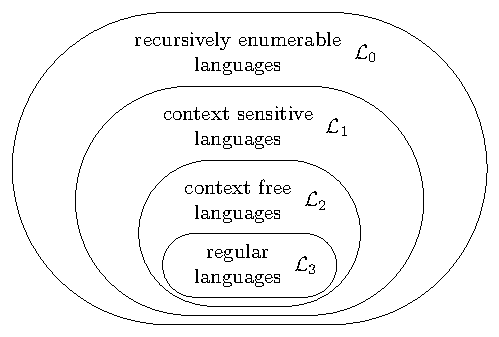
\includegraphics[width=0.75\textwidth]{figures/chomsky-hierarchy.pdf}
\end{figure}

The intricaties of each class are not necessary in the context of this thesis, how ever relugar laguages will be used heavily throughout the rest of this thesis, so they will be explained more in depth.

\begin{table}[h]
\centering
\begin{tabular}{@{}ccl@{}}
\toprule
Grammar         & Language               & Restrictions \\ \midrule
$\mathcal{L}_3$ & Regular                & \todo{todo}             \\
$\mathcal{L}_2$ & Context Free           &              \\
$\mathcal{L}_1$ & Context Sensitive      &              \\
$\mathcal{L}_0$ & Recursively Enumerable &              \\ \bottomrule
\end{tabular}
\caption{An overview of the Chomsky hierarchy classes.}
\label{tab:chomsky-hierarchy}
\end{table}

\subsection{Regular Languages}
As shown above, regular languages are the inner most part of the Chomsky hierarchy, thus they are the most constricted. How ever, regular languages play a crutial role in lexical analysis, more precisely pattern matching. These constrictions lead to many useful closure propetries and decisability properties, mainly membership, which will be introduced shortly.

Regular languges may be defined in multiple equivalent manners such as through finite automata or regular expressions. 

\subsubsection{Finite Automata}

\begin{definition}[Deterministic Finite Automata]
\label{def:dfa}
DFAs are formally defined as 5-tuples
$$ M = (Q, \Sigma, \delta, q_0, F),$$
where
$Q$ is a finite set of states. $\Sigma$ is a finite set of symbols, also know as a input alphabet. $\delta$ is a transition function between states defined as $\delta : Q \times \Sigma \rightarrow Q$. $q_0$ is a initial state, $q_0 \in Q$. And $F$ is a set of final states, $F \subseteq Q$.

If starting in the state $q_0$ and moving left to right over the input string such that during each move a single symbol is consumed from the input string and a transition function for the corresponding state and symbol exists. If after all symbols from the input string have been read and the dfa stopped in a final state, the string is accepted. This is called a deterministic finite acceptor. \todo{rephrase nicer}
\end{definition}


\subsubsection{Regular Expressions} 

\begin{definition}[Regular Expressions]
  \label{def:regular_exp}
\end{definition}



\todo{show equivalence DFA = NFA = $\mathcal{L}_3$}



\begin{figure}[h]
  \caption{Description of a compiler as a single unit.}
  \label{fig:dfa}
  \centering
  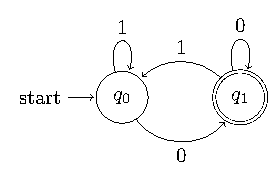
\includegraphics[width=0.75\textwidth]{figures/dfa.pdf}
\end{figure}



  


\section{Compilers}


Today's world undeniably relies on software more than ever before. It is imperative for developers to be able to efficiently write software. Software today is written in programming languages, high-level human-readable notations for defining how a program should run. However, before a program can be run on a system, it has to be translated (or compiled) into low-level machine code, which computers can run. The computer program that facilitates this translation is called a \emph{compiler}. See \cref{fig:compiler}.

\begin{figure}[h]
  \caption{Description of a compiler as a single unit.}
  \label{fig:compiler}
  \centering
  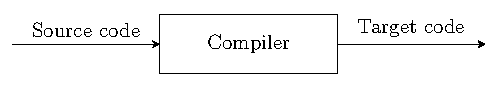
\includegraphics[width=0.75\textwidth]{figures/compiler.pdf}
\end{figure}



Compilers are complex programs. It is helpful to break them down into parts, each handling different tasks, which are chained together to form a compiler. Modern compilers are composed of many phases, such as the Lexical Analyzer, Syntax Analyzer, Semantic Analyzer, Intermediate Code Generator, Machine-Independent Code Optimizer, Code Generator, Machine-Dependent Code Optimizer \cite[p. 5]{dragon}, however this chapter covers the components relevant to this thesis. See relevant stages in \cref{fig:compiler-stages}.


\begin{figure}[h]
  \caption{Overview of relevant compiler stages.}
  \label{fig:compiler-stages}
  \centering
  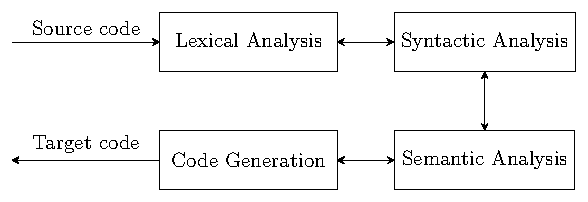
\includegraphics[width=0.75\textwidth]{figures/compiler-stages.pdf}
\end{figure}

\subsection*{Lexical Analysis}
The first stage of a compiler is lexical analysis, also known as a \emph{lexer} or \emph{tokenizer}. For the remainder of this thesis, \emph{lexer} will refer to the lexical analysis stage of a compiler. The lexer consumes a stream of characters, the \emph{source code}, and returns a stream of \emph{tokens}. A \emph{token} is a lexically indivisible unit, for example, the Python keyword \texttt{return}, you cannot divide it further, for example, into \texttt{re} \texttt{turn}. Each token is comprised of characters. The rule that defines which combination of characters constitutes a given token is called a \emph{pattern}. The sequence of characters matching a pattern is called a \emph{lexeme}, the \emph{lexeme} is stored along with the token as a value.

%Lexical analysis may be further divided into two distinct stages, however they are often implemented together. These stages are the \emph{scanner} and \emph{evaluator}.


\subsubsection*{Regular Expressions}
A compact way to represent the patterns accepting tokens are \emph{regular expressions}, which were introduced in \cref{def:regular_exp}. Regular expressions are an algebraic definition of patterns, they specify \emph{regular languages}, $\mathcal{L}_3$

\subsection*{Syntactic Analysis}

\subsubsection*{LL Parser}

\subsection*{Semantic Analysis}

\subsection*{Code Generation}


\chapter{Transpiler Implementation}
\section{Tools \todo{rename}}
\todo{mention python, sphinx, pytest, explain motivation for implementation of own transpiler}

\todo{mention lexer regex implementation}
\todo{mention LL table calculation according to theory}
\todo{write about transformation of ast}


\chapter{Evaluation of Results}
\todo{talk about methodology}
\todo{test examples analyticall vs FDTD}
\chapter{Conclusion}
\todo{compare lumerical and meep}
\todo{test result TBD}




%=========================================================================

% For compilation piecewise (see projekt.tex), it is necessary to uncomment it
% \end{document}

  \else
    % Tento soubor nahraďte vlastním souborem s obsahem práce.
%=========================================================================
% Autoři: Michal Bidlo, Bohuslav Křena, Jaroslav Dytrych, Petr Veigend a Adam Herout 2019

% Pro kompilaci po částech (viz projekt.tex), nutno odkomentovat a upravit
%\documentclass[../projekt.tex]{subfiles}
%\begin{document}

\chapter{Úvod}

Tento text slouží jako ukázkový obsah šablony a současně rekapituluje nejdůležitější informace z předpisů a poskytuje další užitečné informace, které budete potřebovat pro tvorbu technické zprávy ke svojí práci. Než se šablonou budete dále pracovat, je třeba vědět, jak ji správně použít. To je stručně uvedeno v~příloze \ref{jak}.

I když některým studentům pro napsání dobré diplomové práce (bakalářská práce je také diplomová -- dostává se za ni diplom) stačí znát a dodržovat oficiální formální požadavky uvedené ve směrnicích a typografické zásady, často je výhodné před započetím psaní zjistit, jaké jsou osvědčené postupy pro psaní odborného textu a jak si práci usnadnit. Někteří vedoucí svým studentům připravili popisy osvědčených postupů, které vedly k desítkám úspěšně obhájených prací. Výběr nejzajímavějších postupů, které měli autoři této šablony k~dispozici ve chvíli její tvorby, je v níže uvedených kapitolách. Má-li Váš vedoucí svoji stránku s doporučenými postupy, tyto kapitoly můžete vynechat a řídit se pokyny svého vedoucího. Pokud takovou stránku nemá, může být přečtení níže uvedeného textu vhodnou přípravou na konzultaci o plánované struktuře a náplni textu práce.

Diplomová práce je rozsáhlé dílo a tomu odpovídá i technická zpráva. Ne každý je schopen si sednout a jednoduše ji napsat. Je třeba vědět, kde začít a jak postupovat. Jedním z možných přístupů je začít psaním klíčových slov a abstraktu, abyste si ujasnili, co je v~práci nejdůležitější. O tom pojednává kapitola \ref{abstrakt}.

Po sepsání abstraktu se lze pustit do psaní samotného textu technické zprávy. Typicky si nejprve připravíme základní strukturu práce, kterou pak budeme plnit textem. Kapitola \ref{struktura} se zabývá základními informacemi a radami pro psaní odborného textu, které Vám pomohou vyhnout se začátečnickým chybám, a stanovením nadpisů kapitol a přibližných rozsahů jednotlivých částí práce. V závěru kapitoly je pak uveden přístup, kterým si lze psaní technické zprávy značně usnadnit.

Diplomové práce v oblasti informačních technologií mají určitou typickou strukturu. Po~úvodu bude následovat kapitola či kapitoly zabývající se shrnutím současného stavu, který bude v následujících kapitolách zhodnocen a bude navrženo řešení, které bude implementováno a otestováno. V závěru pak budou výsledky vyhodnoceny a bude navržen budoucí vývoj. I když se názvy a rozsahy kapitol v různých pracích liší, vždy tam lze najít kapitoly odpovídající této struktuře. Kapitola \ref{kapitoly} se zabývá obsahy typických kapitol, které se v diplomových pracích z oblasti IT vyskytují. Většina studentů ve svojí práci pravděpodobně využije pouze určitou podmnožinu popsaných kapitol, která je pro jejich práci relevantní. Uvedené popisy a rady mohou pomoci jak s~rozhodnutím, zda danou kapitolu uvést, tak i~s~vnitřní strukturou a samotným obsahem kapitoly.

Za závěrečnou kapitolou práce vždy následuje seznam použité literatury. Citacemi, které tento seznam tvoří, a odkazy na ně se zabývá kapitola \ref{citace}. Byť to tak nezkušený student nemusí vnímat, je seznam použité literatury a odkazy na něj pro práci zcela zásadní. Hodnocení práce s literaturou a citací tvoří jednu z důležitých částí posudku oponenta a bude-li chybět jediná položka, může to vést k hodnocení stupněm F, následnému disciplinárnímu řízení za plagiátorství a k vyloučení z nedokončeného studia. Nesprávná práce se zdroji může mít i další důsledky -- v roce 2018 stála křesla dva členy české vlády. Proto prosím citacím věnujte odpovídající pozornost. 

Po dokončení textu je nutné zjistit, jaké požadavky jsou kladeny na vysokoškolskou kvalifikační práci na FIT VUT v~Brně, a dořešit případné nedostatky. Formální požadavky jsou uvedeny ve směrnicích a na webových stránkách, které jsou zmíněny v kapitole \ref{formality}. Tato kapitola obsahuje i požadované rozsahy jednotlivých typů prací a další vybrané informace z~předpisů a doporučení. V závěru kapitoly je uveden přehled nejčastějších chyb, se kterými se oponenti setkávají a kterým byste se měli vyhnout. Hodnocení formální úpravy práce je pak další z důležitých součástí posudku oponenta.

Po odstranění formálních nedostatků lze práci odevzdat. Před odevzdáním práce si můžete projít kontrolní seznam (tzv. \uv{checklist}) uvedený v příloze \ref{checklist}. Samotné odevzdání listinné i elektronické verze práce je pak popsáno v kapitole \ref{odevzdani}.

V závěrečné kapitole \ref{zaver} je pak uvedeno shrnutí toho, co se lze přečtením tohoto textu dozvědět, a to nejdůležitější, na co je třeba myslet před odevzdáním práce.


\chapter{Abstrakt}
\label{abstrakt}
Pod nadpisem Abstrakt je uvedeno shrnutí práce zabírající prostor maximálně 10 řádků. Z~dobrého abstraktu by mělo být i přes jeho malý rozsah patrné, jaký problém se řešil, jaký přístup k jeho řešení byl v práci použit a jakých výsledků bylo dosaženo. Účelem abstraktu je, aby potenciální čtenář práce již po přečtení abstraktu věděl, zda v práci najde to, co hledá \cite{fitWeb}. Zbytek této kapitoly byl převzat z blogu prof. Herouta \cite{Herout}.
\bigskip

\noindent Za prvé – na abstraktu záleží. Za druhé – není těžké ho napsat. Pojďme na to.

\subsection*{K čemu je abstrakt}
Abstrakt slouží k \bf vyhledávání\rm, společně s názvem dané vědecké práce a seznamem klíčových slov. Tyto části (snad s výjimkou názvu) nejsou přímo součástí textu a nečeká se, že někdo, kdo by zasedl ke čtení dané vědecké práce, bude číst je. To, že práci čte, znamená, že už se dostal za fázi čtení abstraktu. Abstrakt mu slouží ve chvíli, kdy se ještě rozhoduje, \bf zda vůbec \rm text číst.

Když někdo tam venku hledá odpověď na svůj problém, zadá knihovnici nebo dnes spíše vyhledávacímu serveru klíčová slova, která se jeho potíží dotýkají. Na základě shody těchto klíčových slov a klíčových slov uvedených autory dostane seznam názvů prací, které by mu mohly nabízet řešení. Dobře sestavený název práce badateli pomůže vytipovat takové texty, které by mohly mít vztah k jeho problému a mohl by se zajímat o jejich přečtení.

A tady právě přichází na scénu abstrakt. Badatel si čte abstrakt vytipovaných prací a~rozhoduje se, zda práci skutečně chce číst, nebo jestli se v tomto případě jeho filtr založený pouze na jednořádkovém nadpisu zmýlil.

V tuto chvíli obvykle ještě nemá stažené nějaké PDF s celým textem, natož aby měl v ruce vytištěný fascikl. Abstrakty jsou určeny k tomu, aby byly \bf mimo text\rm , aby ležely na serverech agregujících vědecké texty. Proto první pravidlo je, že abstrakt musí fungovat samostatně -- pokud obsahuje odkazy do literatury nebo se odvolává na text (\uv{Výkonnost metody je přehledně shrnuta na straně 51.}), nedělá badateli dobrou službu, což badatel ocení tím, že si o autoru nepomyslí nic hezkého, práci si nepřečte a autora neocituje.

\subsection*{Kdy a jak psát Abstrakt}
Může dávat smysl psát abstrakt na závěr celého psaní -- jako shrnutí a skutečné anotování sepsaného díla. Já jsem vyznavačem opačného přístupu -- abstrakt píšu na samém začátku. Když píšu vědecký článek, začínám sepsáním velkého počtu klíčových slov, jež se textu dotýkají. Bývá jich více, než potom uvedu jako ona charakteristická klíčová slova používaná k indexování. Ujasňuji si tím prostor, kde se článek pohybuje -- o čem je třeba hovořit, co je v textu podstatné, čeho se dotýká. Hned po ujasnění klíčových slov formuluji nadpis a~právě abstrakt. 

Považuji za mimořádně užitečné ujasnit si právě ony čtyři části abstraktu -- Jaký problém se řeší? Jaké řešení práce nabízí? Jaké jsou přesně výsledky? Jaký je jejich význam? Když je toto jasné, text se píše skoro sám. Pokud toto má být nejasné, jak u všech všudy je možné vůbec dát dohromady smysluplnou větu v samém textu?

\subsection*{Doporučená struktura abstraktu}
Abstrakt vědecké práce se může skládat ze čtyř částí a pak být opravdu užitečný. Každá část se bude skládat z nějakých dvou, tří vět, někdy postačí jedna.

V byznysu se vžil slovesný útvar \uv{elevator pitch} -- představení ve výtahu. Ne náhodou jeho struktura připomíná právě doporučovanou strukturu abstraktu. Opravdu, autor odborného textu má do abstraktu napsat právě to, co by říkal o své práci, kdyby na to měl nejvýše dvě minuty a nemohl použít žádných slajdů, obrázků, textu. O čem by tedy měl mluvit?

\paragraph{První část -- Jaký se řeší problém? Jaké je téma? Jaký je cíl textu?}
\begin{itemize}
  \item{Tato práce řeší.}
  \item{Cílem této práce je.}
  \item{Zaměřil jsem se na.}
\end{itemize}
Nepatří sem úvodní pohádky charakteristické pro špatný odborný sloh: \uv{Naše poslední pětiletka staví před nás nové a smělé cíle}, \uv{S rozvojem výpočetní techniky a zejména zobrazovacích zařízení je stále důležitější \ldots} Ty nepatří do dobrého textu nikam, ale do~abstraktu tím méně. Pokud dokážete vyjádřit účel svého textu v jedné větě o pár slovech, udělejte to a nepřidávejte nic navíc. Stručnější zde vždy znamená lepší.

\paragraph{Druhá část -- Jak je problém vyřešen? Cíl naplněn?}
\begin{itemize}
  \item{Zvolený problém jsem vyřešil pomocí toho a toho.}
  \item{V řešení bylo použito metody té, postupu toho a analýzy oné.}
  \item{Práce představuje algoritmus takový, který.}
  \item{Data jsem zpracovával pomocí těch a těchto nástrojů a provedl vyhodnocení takové.}
  \item{Podstatou našeho algoritmu je.}
\end{itemize}

Pokud je podstatou sepisovaného odborného textu nová metodologie (= \uv{jak něco dělat}), patří přesně sem její popis. Pokud se představované řešení skládá ze tří částí, pravděpodobně v této části abstraktu budou tři věty, z nichž každá se bude věnovat jedné části řešení. Dobrý abstrakt v této části bude upřímný a přesný -- nebude si schovávat \uv{odhalování svých tajemství} až do textu. Vágní formulace podstaty řešení v abstraktu obvykle znamená, že autoři buď neumí psát a nebo vlastně nemají o čem -- ani jedno není zrovna výzva ke stažení a čtení mnoha stran textu.

\paragraph{Třetí část -- Jaké jsou konkrétní výsledky? Jak dobře je problém vyřešen?}
\begin{itemize}
  \item{Podařilo se dosáhnout úspěšnosti 87,3\,\%.}
  \item{V práci jsme vytvořili systém, který.}
  \item{Vytvořené řešení poskytuje ty a ty možnosti.}
  \item{Provedeným výzkumem jsme zjistili, že.}
\end{itemize}

Není špatným zvykem uvést v této části konkrétní číslo -- \uv{existující metodu XY jsme zrychlili pětkrát}. Pokud přínos práce není možné shrnout do dvou nebo tří vět, někde je něco velmi špatně a celý text pravděpodobně nestojí za psaní.

\paragraph{Čtvrtá část -- Takže co? Čím je to užitečné vědě a čtenáři?}
\begin{itemize}
  \item{Přínosem této práce je.}
  \item{Hlavním zjištěním je.}
  \item{Hlavním výsledkem je.}
  \item{Na základě zjištěných údajů je možné.}
  \item{Výsledky této práce umožňují.}
\end{itemize}

Při psaní vědeckých článků já sám obvykle bojuji s podobností části třetí a čtvrté. Vskutku, obě hovoří o tom, co jsou výsledky a přínosy textu. Účelem třetí části je jmenovitě a konkrétně jmenovat dosažené výsledky, úkolem části čtvrté je interpretovat jejich význam. Asi ničemu nevadí, když tato dvě sdělení do jisté míry splynou a část třetí a čtvrtá nejen že nemají každá vlastní odstavec, ale prolínají se dokonce ve společných větách.

\paragraph{Nultá část -- O co jde? Kde jsme?}
\begin{itemize}
  \item{Práce je řešena v kontextu tom a tom.}
  \item{Nauka ta a ta se zabývá studiem toho a toho.}
  \item{Stavíme na těchto a oněch nedávných pokrocích v naší oblasti.}
\end{itemize}

Někdy je nutné na sám začátek abstraktu vložit kratičké uvedení kontextu, ve kterém se~celá záležitost vlastně odehrává. Může to být přínosné~u vskutku obskurního a esoterického oboru, který leží stranou hlavního proudu. Obvykle tato část ovšem nebývá nutná a~věty v~ní obsažené bývají prototypy ohavné, rádobyodborné vaty. Je dobrou praxí zapomenout, že se tato část v abstraktu může vyskytovat. Když někdo, kdo je odborníkem v~oboru práce, přece po přečtení abstraktu zavrtí hlavou: \uv{Vůbec nevím, o čem tady můžete psát,} pouze tehdy je vhodné vložit nějaké věty s uvedením kontextu.

\subsection*{Inovace není Ignorance}

Popisuji v tomto textu jakýsi obecný model obecné diplomky. Ještě ke všemu se na začátku zaklínám, že to je můj názor a vkus a jsem zvědavý na názory a vkusy alternativní (což jsem!). Každý diplomant (Mgr. i Bc.) přitom cítí, že jeho diplomka je speciální a výjimečná. Tudíž se nebude držet nějakého schématu, které slouží pro běžné a průměrné diplomky -- tj. pro ty ostatní. Setkávám se s dobrými důvody, proč se od výše naznačeného schématu odchýlit a každoročně některým studentům odchýlení od schématu sám doporučuji. Vskutku, každá diplomka je jedinečná a zvláštní. Kdyby ne, nemusely by se psát, stačilo by je kopírovat. Ovšem vždycky před tím, než vybočíte ze standardního a kanonického způsobu organizování odborného textu, dejte si tu práci ho poznat, pochopit a zvládnout. Způsob vědecké práce, strukturování odborného textu, nebo třeba citování pramenů, může vypadat rigidně a neohrabaně, je to ale zatím ten nejlepší způsob, který jsme jako lidstvo dokázali vymyslet. Pokud ho ovládnete, pochopíte jeho výhody a nevýhody a inovujete ho, je to v pořádku a jste vítáni. Pokud se jím odmítnete zabývat, pravděpodobně neprovedete hodnotnou inovaci, ale vytvoříte \uv{paskvil}.


\chapter{Příprava základní struktury práce} 
\label{struktura}

V této kapitole jsou nejprve uvedeny obecné zásady pro psaní odborného textu a po nich následuje detailnější popis doporučeného postupu přípravy struktury a základní osnovy práce.

Před začátkem psaní textu práce je vždy vhodné zeptat se svého vedoucího, co Vám poradí a zda nemá nějakou svoji aktuální stránku s radami a pokyny. Jeho zaměření bude pravděpodobně odpovídat zaměření Vaší práce a poradí Vám tu nejvhodnější strukturu, které byste se měli držet. Dozví-li se autoři tohoto souboru o další sbírce užitečných rad, jistě sem v budoucnu budou zařazeny.

Tento text se zaměřuje na obecná doporučení a obecnou strukturu práce, kterou je vždy potřeba  modifikovat a popřemýšlet o ní na základě konkrétního zadání \cite{Cernocky}.

\section{Užitečné rady pro psaní odborného textu}

Následující pokyny jsou dostupné též na školních webových stránkách~\cite{fitWeb}. Přehled základů typografie a tvorby dokumentů s využitím systému \LaTeX{} je uveden v~knize od~Jiřího Rybičky~\cite{Rybicka}.

Hodnocenou součástí potenciálního inženýra je mimo jiné i jazyková kvalita a čistota. Naším cílem je vytvořit jasný a~srozumitelný text. Vyjadřujeme se proto přesně, píšeme dobrou češtinou či slovenštinou (případně angličtinou) a~dobrým slohem podle obecně přijatých zvyklostí. Předpokládá se dodržování pravopisných norem zvoleného jazyka práce a dodržování odborného názvosloví. Slangové výrazy jsou nepřípustné. Při pochybnostech o~překladu či přepisu cizích pojmů využijte literatury dostupné v knihovně FIT. 

Text má upravit čtenáři cestu k~rychlému pochopení problému, předvídat jeho obtíže a~předcházet jim. Dobrý sloh předpokládá bezvadnou gramatiku, správnou interpunkci a~vhodnou volbu slov. Snažíme se, aby náš text nepůsobil příliš jednotvárně používáním malého výběru slov a~tím, že některá zvlášť oblíbená slova používáme příliš často. Pokud používáme cizích slov, je samozřejmým předpokladem, že známe jejich přesný význam. Ale i~českých slov musíme používat ve správném smyslu. Např. platí jistá pravidla při používání slova {\it zřejmě}. Je {\it zřejmé} opravdu zřejmé? A~přesvědčili jsme se, zda to, co je {\it zřejmé}, opravdu platí? Pozor bychom si měli dát i~na příliš časté používání zvratného se. Například obratu {\it dokázalo se, že \ldots{}} zásadně nepoužíváme.

Za pečlivý výběr stojí i~symbolika, kterou používáme ke {\it značení}. Máme tím na mysli volbu zkratek a~symbolů používaných například pro vyjádření typů součástek, pro označení hlavních činností programu, pro pojmenování ovládacích kláves na klávesnici, pro pojmenování proměnných v~matematických formulích a~podobně. Výstižné a~důsledné značení může čtenáři při četbě textu velmi pomoci. Je vhodné uvést seznam značení na začátku textu. Nejen ve značení, ale i~v~odkazech a~v~celkové tiskové úpravě je důležitá důslednost.

S tím souvisí i~pojem z~typografie nazývaný {\it vyznačování}. Zde máme na mysli způsob sazby textu pro jeho zvýraznění. Pro zvolené značení by měl být zvolen i~způsob vyznačování v~textu. Tak například klávesy mohou být umístěny do obdélníčku, identifikátory ze~zdrojového textu mohou být vypisovány {\tt písmem typu psací stroj} a~podobně.

Uvádíme-li některá fakta, neskrýváme jejich původ a~náš vztah k~nim. Když něco tvrdíme, vždycky výslovně uvedeme, co z~toho bylo dokázáno, co bude dokázáno v~našem textu a~co přebíráme z~literatury s~uvedením odkazu na příslušný zdroj. V~tomto směru nenecháváme čtenáře nikdy na pochybách, zda jde o~myšlenku naši nebo převzatou z~literatury.

Abychom mohli napsat odborný text jasně a~srozumitelně, musíme splnit několik základních předpokladů:
\begin{itemize}
\item Musíme mít co říci,
\item musíme vědět, komu to chceme říci,
\item musíme si dokonale promyslet obsah,
\item musíme psát strukturovaně. 
\end{itemize}

\subsection*{Musíme mít co říci}
Nejdůležitějším předpokladem dobrého odborného textu je myšlenka. Je-li myšlenka dost závažná, tak přetrvá, i když je neobratně a zmateně podaná. Chceme-li však myšlenku podat co nejvýstižněji a ušetřit tak čtenáři čas, musíme dodržet určité zásady, o kterých pojednáme dále.

\subsection*{Musíme vědět, komu to chceme říci}
Dalším důležitým předpokladem dobrého psaní je psát pro někoho. Píšeme-li si poznámky sami pro sebe, píšeme je jinak než výzkumnou zprávu, článek, diplomovou práci, knihu nebo dopis. Podle předpokládaného čtenáře se rozhodneme pro způsob psaní, rozsah informace a~míru detailů.

\subsection*{Musíme si dokonale promyslet obsah}
Musíme si dokonale promyslet a~sestavit obsah sdělení a~vytvořit pořadí, v~jakém chceme čtenáři své myšlenky prezentovat. 
Jakmile víme, co chceme říci a~komu, musíme si rozvrhnout látku. Ideální je takové rozvržení, které tvoří logicky přesný a~psychologicky stravitelný celek, ve kterém je pro všechno místo a~jehož jednotlivé části do sebe přesně zapadají. Jsou jasné všechny souvislosti a~je zřejmé, co kam patří.

Abychom tohoto cíle dosáhli, musíme pečlivě organizovat látku. Rozhodneme, co budou hlavní kapitoly, co podkapitoly a~jaké jsou mezi nimi vztahy. Diagramem takové organizace je graf, který je velmi podobný stromu, ale ne řetězci. Při organizaci látky je stejně důležitá otázka, co do osnovy zahrnout, jako otázka, co z~ní vypustit. Příliš mnoho podrobností může čtenáře právě tak odradit jako žádné detaily.

Výsledkem této etapy je osnova textu, kterou tvoří sled hlavních myšlenek a~mezi ně zařazené detaily.

\subsection*{Musíme psát strukturovaně} 
Musíme začít psát strukturovaně a~současně pracujeme na co nejsrozumitelnější formě, včetně dobrého slohu a~dokonalého značení. 
Máme-li tedy myšlenku, představu o~budoucím čtenáři, cíl a~osnovu textu, můžeme začít psát. Při psaní prvního konceptu se snažíme zaznamenat všechny své myšlenky a~názory vztahující se k~jednotlivým kapitolám a~podkapitolám. Každou myšlenku musíme vysvětlit, popsat a~prokázat. Hlavní myšlenku má vždy vyjadřovat hlavní věta a~nikoliv věta vedlejší.

I k~procesu psaní textu přistupujeme strukturovaně. Současně s~tím, jak si ujasňujeme strukturu písemné práce, vytváříme kostru textu, kterou postupně doplňujeme. Využíváme ty prostředky DTP\footnote{Desktop publishing (DTP) -- tvorba tištěného dokumentu na počítači.} programu, které podporují strukturovanou stavbu textu (předdefinované styly pro nadpisy a~bloky textu).

\subsection*{Nikdy to nebude naprosto dokonalé}
Když jsme už napsali vše, o~čem jsme přemýšleli, uděláme si den nebo dva dny volna a~pak si přečteme sami rukopis znovu. Uděláme ještě poslední úpravy a~skončíme. Jsme si vědomi toho, že vždy zůstane něco nedokončeno, vždy existuje lepší způsob, jak něco vysvětlit, ale každá etapa úprav musí být konečná.

\section{Komu se píše diplomka}
Tato podkapitola byla převzata z blogu prof. Herouta \cite{Herout}.

\bigskip
\noindent \bf Pište svou diplomku pro studenta, který má na Vaše dílo navázat. \rm
\bigskip

Představte si, že na Vaší práci bude dál pracovat student Franta, asi tak stejně chytrý jako Vy sami. Máte teď čtyři hodiny na to, abyste mu svou práci ukázali, zasvětili ho do~všeho, co je potřeba, a on pak bude pokračovat sám. Franta je studentem stejné školy jako Vy a~ví asi tolik, co průměrný student, není žádným super odborníkem na obor Vaší diplomky, ale rozhodně není hloupý a řešeného tématu se neštítí. Franta, tak jako Vy, se~o~tom, že bude po Vás pokračovat, zrovna dozvěděl, takže ještě neměl čas si něco k~tématu nastudovat.

Bude dobré začít tím, že se Franta dozví, co je cílem práce, proč se to celé dělá, co mají být výsledky.

Nikdo soudný by hodinu z vyměřeného času s Frantou nestrávil řečněním typu: \uv{\mbox{Internet} byl vytvořen americkou armádou v roce 1962, pak v roce 1991 v CERNu udělali www, a~nyní se používá v nejrůznějších oblastech lidské činnosti.} (to vše na šesti stranách s~mnoha odkazy a obrázky).
Franta obvykle nepotřebuje několikastránkové skriptum o detailech barevných modelů pro reprezentaci obrázků, historii a detaily Houghovy transformace, kompletní popis vrstev referenčního modelu ISO/OSI, ani řadu koláčových grafů o~zastoupení jednotlivých mobilních platforem na trhu za posledních deset let.
Franta potřebuje nasměrovat na~cenné zdroje, které Vám při řešení pomohly, a chce letmý popis nástrojů a~algoritmů, které byly nutné pro řešení: \uv{Je potřeba nástroj XY, který slouží k tomuhle a~tamtomu, hlavně jeho modul PQ, který se používá tehdy a~tehdy. Nejlepší je k tomu tato dokumentace.}

Řekněte Frantovi hodně o tom, co se při řešení osvědčilo a co pomáhalo, ale upozorněte ho i na to, co nejdřív vypadalo jako dobrý nápad, ale pak se ukázalo jako zbytečné nebo nefunkční.

Dobře dávkujte úroveň detailu. Nějakou optimalizační fintu rozeberete ve zdrojovém kódu řádek po řádku, nějaký pomocný modul přejdete jedním odstavcem s popisem vstupů a výstupů a odkazem na použitou knihovnu.

Představte si průběh toho čtyřhodinového sezení s Frantou.
\begin{itemize}
  \item{O čem byste asi mluvili na začátku, kdy se Franta teprve začíná orientovat?}
  \item{Co jsou věci, které by rozhodně měly zaznít?}
  \item{Jaké obrázky byste v průběhu sezení malovali?}
  \item{Na co by se Franta vyptával, protože je to důležité a přitom to není samozřejmé?}
  \item{Na jaká omezení a nedodělanosti byste Frantu potřebovali upozornit, aby neupadl do~nějaké pasti?}
  \item{Jak vlastně Franta může pokračovat? Co jsou otevřené záležitosti, které by ještě stálo za to vyzkoušet a vylepšit?}
  \item{Co byste říkali úplně první (úvod) a úplně poslední (závěr) minutu sezení?}
\end{itemize}


\section{Struktura diplomové práce -- Pět kapitol}
Není-li dále uvedeno jinak, tato podkapitola byla převzata z blogu prof. Herouta \cite{Herout} (částečně inspirovaného knihou, kterou napsal Jean-Luc Lebrun \cite{Lebrun2011}) a z dokumentu na osobní stránce prof. Zemčíka~\cite{Zemcik}.
\bigskip

Diplomová práce je činnost, kterou student vyvíjí po dva semestry studia a pak o ní sepíše knížečku. Rozšířená terminologická chyba je, že se té knížečce, která je o činnosti sepsaná, říká diplomová práce. Ta knížečka je ve skutečnosti technická zpráva o provedené roční činnosti a diplomová práce je ta roční činnost.

Diplomantova roční činnost zahrnuje za prvé studium: \uv{Co už v oblasti mého zadání existuje? Jak to dělají jiní?} V rámci diplomky člověk dále nějaké věci vymyslí a navrhne: \uv{Zadaný problém lze řešit tak a nebo tak, já k němu přistoupím tímto způsobem, protože na~zvolené platformě je to nejefektivnější.} To, co řešitel navrhl, by měl po sobě ověřit tím, že to implementuje a vyhodnotí: \uv{Pro implementaci jsem zvolil ty a ty nástroje, celý systém rozvrhl do takových modulů. Výsledek je takhle rychlý, má takovou úspěšnost a~reakce uživatelů jsou takové a takové.}

Základní struktura diplomové práce podle prof. Herouta tedy je:
\begin{enumerate}
  \item{Úvod (1 strana)}
  \item{Co bylo třeba vystudovat (vč. zhodnocení současného stavu; 40\,\% rozsahu)}
  \item{Nové myšlenky, které tato práce přináší (30\,\%)}
  \item{Implementace a vyhodnocení (30\,\%)}
  \item{Závěr (1 strana)}
\end{enumerate}

Není chybou, když text má právě 5 takových kapitol, není ani chybou, když je některá z~nich rozdělena na dvě části -- o tom dále. Obvykle je velkou chybou, když tam některá část chybí, nebo má nápadně odchylný rozsah. Názvy kapitol nemusí kopírovat tuto strukturu. Samozřejmě, samotný obsah práce je nadřazen všem zásadám a pokud tedy bude dobrý důvod strukturu porušit, tak to udělejte.

Na této základní struktuře se řada vedoucích shoduje, byť různí vedoucí doporučují rozdílné názvy kapitol a např. zhodnocení současného stavu lze umístit nejen do 2., ale i~do~3. kapitoly jak to doporučuje prof. Zemčík:
\begin{enumerate}
  \item{Úvod (1--2 strany)}
  \item{Shrnutí dosavadního stavu (40--50\,\% celkového rozsahu)}
  \item{Zhodnocení současného stavu a návrh řešení (3--5 stran)}
  \item{Popis vlastní práce (cca 40\,\% celkového rozsahu)}
  \item{Závěr (max. 1 strana)}
\end{enumerate}

Názory vedoucích se dle zaměření práce liší i v rozsazích, jak je vidět např. v~doporučeních dr. Berana \cite{Beran}:
\begin{enumerate}
  \item{Úvod (1 stránka)}
  \item{Teorie (1/3 stran)}
  \item{Návrh řešení (1/3 stran)}
  \item{Realizace, experimenty a vyhodnocení (1/3 stran)}
  \item{Závěr (1 stránka)}
\end{enumerate}

U prakticky zaměřených prací, pro která jsou zásadní data a uživatelská rozhraní, lze využít doporučení od doc. Černockého \cite{Cernocky}:
\begin{enumerate}
  \item{Úvod (jednotky stran)}
  \item{Teoretická část (cca 10 stran)}
  \item{Data (jednotky stránek)}
  \item{Popis Vašeho algoritmu a jeho testování (cca 10 stran)}
  \item{Návrh a implementace (pár stran)}
  \item{Uživatelské rozhraní (pár stran)}
  \item{Testování (cca 10 stran)}
  \item{Závěr (jednotky stran)}
\end{enumerate}

\section{Diplomka -- komiksová edice}
Tato podkapitola byla převzata z blogu prof. Herouta \cite{Herout}.

Diplomka (bakalářka je taky diplomka) je poměrně komplexní dílo. Skládá se z velkého počtu písmenek. A ta písmenka nejsou jen tak za sebou, ale jsou uspořádána hierarchicky do~kapitol. Celé to musí mít nějakou logiku, nějaký sled -- čtenář se musí nejdřív dozvědět jedny věci, aby mu pak šlo přesvědčivě předat věci jiné. Musí tam být obrázky, tabulky, vzorce; zároveň si tyto ne-textové věci musí s okolním textem povídat a navzájem se doplňovat. Musí se zcela pokrýt oficiální zadání, a vše musí být doručeno k nějakému přesnému datu, vytištěné a svázané. Pokud, nad to všechno, má být diplomka dobrá, musí to všechno být uděláno dobře. Když se peče koláč z deseti surovin a jedna z nich je zkažená, celý koláč bude hnusný. Musí klapnout všechno.

\subsection*{Jak to všechno pohlídat? Odkud zaútočit?}
Když s kolegy píšeme článek (poslední dobou asi tak pořád), v hodně rané fázi připravíme něco, čemu říkáme \uv{Comics Edition}. Děláme to jednak proto, že já na tom trvám, a dvak proto, že nám to dosti pomáhá. Třeba to pomůže i Vám s diplomkou.

Nejprve si ujasněte odpovědi na následující otázky:
\begin{itemize}
  \item{Jak byste vystihli podstatu svého řešení ve třech až pěti krátkých větách?}
  \item{Jaké jsou silné stránky Vašeho řešení?}
  \item{Jaké jsou konkrétní argumenty, že to, co jste udělali, je dobré?}
  \item{Kdyby chtěl někdo být na Vaši práci zlý -- co by vytkl?}
  \item{Co byste mu odpověděli?}
  \item{Jaká klíčová slova by měl člověk zadat do vyhledávače, aby Vaše diplomka byla relevantní odpovědí?}
\end{itemize}

Pokud máte, můžeme jít na věc \ldots

\subsection*{Hned založit TEN dokument}
Občas vídám postup, že někdo píše \uv{předběžnou} verzi diplomky do nějakého poznámkovadla. Je to za prvé práce navíc a za druhé zbytečná. Je třeba hned založit dokument, ve~kterém svůj boj dokončíte, a ze kterého výsledek vytisknete.

\subsection*{Nadpisy kapitol}
Důležitou součástí komixového vydání, o něž se tu snažíme, jsou nadpisy kapitol. Vložte je do dokumentu. Vložte je tak, jak budou z hlediska formátování -- žádné provizorní seznamy: \uv{Já to pak předělám}. Chcete vidět, jak přesně to bude vypadat, jak se vyloupne celý automaticky sestavený obsah. Vložte je jak budou z hlediska jejich znění. Nadpis kapitoly říká, co v kapitole bude. Nadpisy kapitol tvoří kostru celého díla, již pak obalujete masem a kůží textu a obrázků.

Ze všech slov, která jsou v diplomce, jsou slova v nadpisech \textbf{ta nejdůležitější}. Věnujte jim opravdu mimořádnou pozornost.

\subsection*{Obrázky}
Obrázek vydá za tisíc slov. Prošel jsem 8 posledních článků, jež jsem spoluautoroval. Dohromady mají 80 stran, obsahují 87 obrázků a 17 tabulek, tj. 1,3 vizuálního sdělení na~stránku (včetně stránek obsahujících reference do literatury, úvodních stránek s abstrakty a vůbec všeho). Mnohé obrázky (tak půlka) se ve skutečnosti skládají z několika podobrázků, zvlášť odkazovaných. Těch jsem v řečených 8 článcích napočítal 221, tj. v průměru 3 vizuály na~stranu. Taková je moje představa o roli obrázků v odborném textu. Nemyslím si, že by mohla existovat vážně míněná diplomka, která by měla \uv{příliš mnoho obrázků}.

Již v rané verzi komixového vydání diplomky hleďte promyslet, kde se obrázky budou vyskytovat a jaké. Obrázky ještě nemusíte mít hotové. Zdaleka. Ještě nevíme, co přesně na~obrázku bude. Ještě nevíme, jaký pod ním bude popisek. Co víme je, že tu nějaký takový obrázek bude a že se bude skládat z více podobrázků a tak ho hned vložíme. Zabere to tak minutu (vektorovou podobu \uv{TODO Image} máme už dávno uloženou a je součástí této šablony) a hned se víc rýsuje, jak text bude vypadat. 
U některých obrázků už dokonce máme představu, jak budou vypadat -- konceptuálně. Nakreslíme na papír nebo na tabuli, vyfotíme mobilem, obrázek vložíme, aby držel místo tomu, jenž přijde po něm a bude nakreslený pořádně (vektorově v Inkscape\footnote{\url{https://inkscape.org}} nebo vygenerovaný Gnuplotem\footnote{\url{http://www.gnuplot.info/}}).

Jen tak na okraj: Obrázek vydá za tisíc slov. Hloupý obrázek vydá za tisíc hloupých slov. A když už jsme u těch obrázků: Kdo vkládá věci, které by měly být vektorové (schémata, grafy, nákresy, diagramy, prakticky všechno kromě fotek a~snímků obrazovek), jako rastrové obrázky, a kdo vkládá snímky obrazovek (a podobné věci, které mají být přesně) se ztrátovou kompresí (obvykle JPEG), nemůže očekávat pozitivní hodnocení práce.

\subsection*{Objem textu}
Zrovna tak jako vkládáme obrázky, které ještě nemáme, vkládáme i text, který ještě nemáme. V \LaTeX{}u je na to krásný příkaz \texttt{\textbackslash Blindtext}\footnote{Stručný tutorial: \url{https://texblog.org/2011/02/26/generating-dummy-textblindtext-with-latex-for-testing/}}. Kdo ho (ke své škodě) nechce nebo neumí používat, použije \url{http://lipsum.com}. Pomůže pisateli tušit přibližný rozsah celého díla, hustotu obrázků v textu a další charakteristiky textu při pohledu shůry. Vytvořit si takový odhad trvá třeba 5 minut. Pro orientaci v rozdělaném textu je rozumné tento nijaký text vybarvit šedou barvou (inteligent si na to udělá příkaz, ať se pak barva snadno jednotně změní pro celý dokument). Zkušenost říká, že bez barev v tom člověk začne mít slušný nepořádek -- co už je hotové, co ne, na čem je potřeba pracovat. Je radno investovat pár minut do zprovoznění balíčku pro barvení textu. V rámci této šablony můžete použít příkaz \verb|\todo|, např. \todo{Toto je třeba dokončit}. 

Geneze každé kapitoly ať začíná tím, že obsahuje třeba 3-5 kusů TODO a nějaké to Lorem ipsum. Každé TODO se pak postupně transformuje na větší počet TODO menšího rozsahu, nebo na text, na obrázek, další podkapitoly, cokoliv. TODO střídavě přibývají a~ubývají, práce se přitom vždycky o kousek pohne.

\subsection*{Jak s tím celým pracovat}
Když na to člověk sedne a \LaTeX{} zrovna nemá špatný den, za hodinu je hotová diplomka (bakalářka je taky diplomka) o správném počtu stran, obsahující představu, co kde bude. Začíná se podobat výsledku, který má přijít až za nějakou dobu, po nějaké práci.

Dokument pak už v zásadě nenarůstá, ale transformuje se. Je velký rozdíl sednout si před prázdnou bílou obrazovku a \uv{psát diplomku} a vzít si jedno TODO a napsat místo něj odstavec. To první je těžké a někdy to prostě nejde. To druhé jde: má to svůj začátek a konec. Ví se, co se má udělat.

Pořád platí, že diplomka se nenapíše sama, ale jde to lépe a výsledek má spíše hlavu a~patu.

\section{Jak pojmenovat kapitoly}
Dobře publikovat neznamená jen posypávat co nejvíc papíru co nejvíce písmenky. Renomé vědce vzniká vlastně až tím, že jinému vědci je jeho práce natolik užitečná, že ho cituje ve~své práci. Proto je potřeba, aby svůj článek napsal dobře: nikdo nebude citovat práci, která je humpolácky napsaná, protože by se sám shodil. 
Humpolácky napsaný článek ovšem nikdo nebude citovat už z toho důvodu, že \bf ho nenajde\rm . Už dávno před nějakým internetovým SEO vědci používali při psaní různé \uv{fligny} tak, aby je další vědec, když dělá svoji rešerši, zařadil mezi svůj materiál, jejž přečte, z něhož si nadělá poznámky a který -- nakonec a~logicky -- ocituje ve svém díle.

Na světě je moře článků. Když vědec Tonda hledá materiál relevantní pro svou práci, zadá klíčová slova (kdysi papírově do knihovny, nyní elektronicky do příslušného vyhledávače) a vypadne mu hromada nálezů -- tj. názvů. První krok, aby článek někdo ocitoval, je mít dobrý název. Tak dobrý, aby Tondu zaujal a on si název rozkliknul ve snaze zjistit více. Název je \bf prvním filtrem\rm . 

Články, jež prošly prvním filtrem, si Tonda rozklikne. To znamená, že vidí abstrakt článku. Abstrakt je \bf druhým filtrem \rm a hodně na něm záleží. Je to jako dostat se do~druhého kola pohovoru k vysněné práci. 

Když tedy Tondu zaujme nadpis i abstrakt, stáhne si celé PDF článku a rychle ho proskroluje, aby si udělal představu: vytiskne ho, nebo okno s článkem zavře a bude se věnovat desítkám jiných? To je \bf třetí filtr \rm a je to jako být mezi pár posledními uchazeči o~práci snů. Na co se Tonda dívá ve třetím kole, během svého skrolování? Na vizuály, tj. na~obrázky, tabulky, vzorce, a právě na nadpisy kapitol. Projde Váš článek třetím filtrem? Bude s ním Tonda pracovat? Na obrázky se zaměříme jindy, tato podkapitola je o nadpisech.

S diplomkami to může být trochu jinak. Ne každý pisatel diplomky stojí o to, aby ji lidé četli. Tušíme, že existují tací, kteří si přejí spíše pravý opak. Pojďme ale v tomto návodu pracovat s hypotézou, že pisatel chce napsat dobrý text, který by mohl být lidstvu užitečný a stojí za čtení. Tj. za který je možné dostat rozumnou známku.

\subsection*{Klíčová slova -- půl úspěchu}
Jedna z nejlepších rad pro psaní článků (a obecně odborného textu), kterou jsem kdy slyšel, není úplně intuitivní a samozřejmá.
\bf Napište si klíčová slova, jež by člověk měl napsat do vyhledávače, aby mu vypadlo Vaše dílo jako relevantní odpověď. \rm 
Popusťte uzdu fantazii, klidně to vezměte ze široka. Přemýšlejte o aplikacích Vaší práce. O souvislostech. Sepište všechna klíčová slova, bude to na několik řádků. Klíčové slovo je i sousloví -- typicky dvou nebo tří slov. Vyberte z nich ta důležitá. K tomu je potřeba intuice a zkušenost. Kde ty vzít, nevím, ale vždycky se můžete s někým (např. vedoucím práce) poradit. Až budete psát svůj třicátý odborný text, půjde to celkem hladce.

\bf Všechna důležitá klíčová slova se musí objevit v nadpisu článku nebo v nadpisech kapitol. \rm 

\subsection*{Příliš obecný nadpis, příliš specifický nadpis}
Proč to s těmi klíčovými slovy? Protože nadpisy jsou směrovníky, ukazatele, které ukazují: \uv{Co hledáš, je tady!} Aby někdo o text stál, musí se v něm zorientovat. Potřebuje vědět, že text nabízí odpovědi na některé jeho otázky. Nadpisy mu v tom můžou pomoct, nebo ho přesvědčit o tom, že o text vlastně nestojí. Kdo si při stěhování napíše na všechny svoje krabice od banánů: \uv{RŮZNÉ VĚCI}, bude mít pravdivé a formálně správné popisky, ale nemusel nic psát. Obecný popisek k ničemu není.

Jednoslovný nebo dvouslovný nadpis kapitoly jsou obvykle podezřelé z toho, že jsou příliš obecné -- s výjimkou úvodu a závěru, kde názvy kapitol jsou kanonické (dané vyhláškou). Máte-li ve své práci jednoslovné nadpisy kromě dvou řečených, pravděpodobně je máte špatně. Název kapitoly, který by šel použít u jiné práce stejného oboru, třeba \uv{Implementace systému}, \uv{Základ zpracování obrazu}, \uv{Principy uživatelských rozhraní}, je podezřelý z~toho, že je příliš obecný. Lepší obvykle bude \uv{Implementace systému pro sledování pohybu much}, \uv{Algoritmy pro detekci objektů a sledování jejich trajektorií}, \uv{Principy uživatelských rozhraní jednoduchých webových systémů}.

Název kapitoly, který by šel použít na úplně rozdílných školách, je prakticky vždycky špatně -- příliš obecný. Nadpis \uv{Teorie} by mohl být použit na lesnické univerzitě, v IT, na~právech, na vysoké škole mlékárenské a sýrárenské. Je špatně. Nadpis \uv{Studium existujících řešení} je špatně. \uv{Průzkum dostupných technologií} je špatně. Ještě jsem neviděl nadpis, který by byl příliš specifický a nemyslím, že by něco takového mohlo existovat. Může být špatně -- tedy nevystihovat, co se v kapitole nachází. Pokud ale vystihuje, nemůže být příliš specifický.

Nevybízím tím k nadpisům na pět řádků. Většina dobrých a specifických nadpisů bude na jediném řádku a budou mít v průměru kolem pěti slov. Tu a tam nadpis přeteče na~druhý řádek a bude k tomu dobrý důvod. Sestavit dobré nadpisy -- dosti specifické a přitom ne~příliš dlouhé -- není lehké, ale vyžaduje to přemýšlení. Jako každá lidská činnost, která má za něco stát.

\subsection*{Zkratky v nadpise}
Zkratky v nadpise nemají co dělat, pokud nejsou úplně super-notoricky známé (ČR, AIDS, IT).

Je možné v první kapitole vysvětlit nějaký pojem a uvést, že dále se bude vyskytovat ve~zkratce. Je možné tuto zkratku používat dále v textu druhé kapitoly bez dalšího vysvětlení. Není ale možné tuto zkratku používat v nadpise druhé kapitoly, protože nadpisy čte vědec Tonda už ve třetím filtru při rozhodování, jestli se vůbec do první kapitoly pustí. Pokud Tonda při rychlém skenování článku narazí na něco, co v něm vzbudí dojem, že text je nějaký divný, nesrozumitelný, vlastně neví, co se tam píše (to je případ zkratky v~nadpise), článek zavře a už ho neotevře.

Odkazy do literatury a odkazy na další objekty v článku (obrázky, nadpisy, \ldots) do~nadpisu nepatří a ještě jsem neviděl případ, kdy by tam byly potřeba (a to už jsem viděl hodně případů, kdy se tam vyskytovaly).

\section{Obecné rady zkušených vedoucích}

Tato podkapitola obsahuje vybrané rady od dalších zkušených vedoucích, pod jejichž vedením již byly obhájeny stovky prací a kteří věnovali nemalé úsilí sepsání svých rad a jejich vystavení na web. Pro kompletní texty neváhejte navštívit jejich stránky, které naleznete v~literatuře \cite{Beran}, \cite{BeranPDF}, \cite{Cernocky} a \cite{Zemcik}.

\subsection*{Obecné rady dle dr. Berana}
Tato podkapitola byla převzata ze stránek dr. Berana \cite{Beran}, \cite{BeranPDF}.

Jak psát/nepsát
\begin{itemize}
  \item{Kapitoly číslujte maximálně do druhé úrovně, nadpisy nižších úrovní volte jako nečíslované a neuvádějte je v obsahu, výsledná práce i obsah budou mnohem přehlednější.}
  \item{Logické členění -- každý celek -- celá práce, každá kapitola, každá podkapitola má: úvod, stať a závěr:
    \begin{itemize}
      \item{úvod -- sděluje, co je obsahem celku, co se dočteme, co se řeší, uvádí do kontextu,}
      \item{stať -- řeší kontext, problém, detailně specifikuje problém, způsob řešení, postup řešení, výsledek řešení,}
      \item{závěr -- rekapituluje úlohu, shrnuje dosažené výsledky a jejich podstatu, uzavírá celek.}
    \end{itemize}}
  \item{Jedná se o technický text, nedoporučuji příliš mnoho osobních pocitů a \uv{povzdechů}.}
  \item{Nepoužívejte množné číslo \uv{MY} jsme udělali, chtěli apod.
    \begin{itemize}
      \item{používejte buď trpný rod, \uv{testy byly provedeny} namísto \uv{my jsme provedli testy} -- zejména v teoretické části, kdy jde o převzaté myšlenky,}
      \item{tam, kde chcete zdůraznit, že se jedná o Váš přínos, Vaši práci, Váš nápad apod. použijte \uv{já} -- návrh řešení, experimenty, realizace,}
      \item{protože MY (já-Vy, Vy-čtenář, Vy-svět) jsme nic neudělali, VY jste udělal(a).}
      \item{(To, že někde používáte nápady vedoucího, neřešte, to se očekává, je to Vaše práce na~jeho téma.)}
    \end{itemize}}
  \item{U převzatých obrázků/myšlenek/tabulek použijte \bf citaci zdroje\rm }.
  \item{Každý \bf nadpis \rm (kapitoly či podkapitoly) by měl být následován odstavcem textu, který čtenáře informuje, co se dočte v následující části, a který čtenáře uvede do~následující problematiky.}
  \item{Nepodceňujte úvod a závěr.}
\end{itemize}


\subsection*{Obecné rady od doc. Černockého}

Tato podkapitola je převzata ze stránek doc. Jana Černockého \cite{Cernocky}.

\begin{enumerate}
  \item{Přečtěte si pár dobrých DP/BP a snažte se vstřebat, jak taková dobrá práce vypadá. Příklady Vám rád dá Váš vedoucí.}
  \item{\textbf{Čeština/Slovenština nebo English?}
    \begin{itemize}
      \item Pokud umíte slušně anglicky a Vaše práce má potenciál být čtena někde jinde než na FIT VUT (součást mezinárodního projektu, práce pro nadnárodní firmu, popis SW, který chcete dát na GooglePlay, atd. atd.), velmi doporučuji psát anglicky. Můžete si 100x říkat, že to pak z češtiny přeložíte, ale už na to nikdy není čas. Navíc nemusíte psát háčky a čárky.
      \item  Pokud pracujete na BP/DP lokálního významu a víte, že Vaše angličtina za~moc nestojí, doporučuji naopak ušetřit sobě i vedoucímu a oponentovi utrpení a psát česky nebo slovensky. Rady pro psaní práce v angličtině a chyby, kterých se studenti často dopouštějí, najdete v~příloze~\ref{anglicky}. 
    \end{itemize}}
  \item{Nemějte strach z toho, že budete mít málo stran! Nerozepisujte se zbytečně, nekopírujte zbytečné věci z Wikipedie -- jen tím naštvete Vašeho vedoucího a oponenta. Pokud budete následovat doporučenou strukturu a budete psát o tom, co jste skutečně udělali, budete mít na závěr dost kvalitního materiálu. }
  \item{Pište průběžně -- nemusíte psát přímo text technické zprávy se vším možným formátováním, ale mějte aspoň nějaký soubor README, kam si budete značit, na čem děláte, průběžné výsledky, co jste četli, co jste použili, o čem to zhruba je atd. Důrazně varuji před systémem \uv{hrnu práci, pak to celé napíšu} -- za půl roku už vůbec nebudete vědět, co jste dělali, a budete si na to (v lepším případě) horko těžko vzpomínat, v horším případě si to budete muset zopakovat. Průběžné psaní Vám také pomáhá strukturovat Vaší technickou zprávu.}
  \item{Používejte kontrolu pravopisu (spell-checker). Ušetřete vedoucího a oponenta opravování hloupých chyb (překlepů apod.). MS Word má kontrolu pravopisu dobrou, v~Linuxu je slušný ispall/aspell/hunspell (volá se např. z populárního textového editoru Emacs). Některé nástroje jsou nepoužitelné, např. ten v PSPadu propouští chyb jak ryb.}
	\item{Vedoucího průběžně seznamujte s aktuálním stavem práce a sdílejte s ním pracovní verze. Vedoucí by měl práci vidět zavčas! -- nejpozději přibližně 14 dní před odevzdáním, nejlépe průběžně po kapitolách (tabulky s výsledky/závěry třeba nemusí být ještě úplně hotové). Vedoucí Vám ji poškrtá, Vy se na něho naštvete, co si to dovoluje nad mým (přece tak krásným!) dílkem, za~půl dne vychladnete a zjistíte, že má vlastně pravdu, opravíte a další verze již bude mnohem kvalitnější. Pokud toto neuděláte a~odevzdáte verzi, kterou jste četl(a) jen Vy, případně nikdo, dostane \uv{plnou palbu} Vašich chyb oponent a podle toho bude vypadat jeho hodnocení.}
\end{enumerate}


\subsection*{Obecné rady od prof. Zemčíka}
Tato část textu je převzata z dokumentu na stránce prof. Zemčíka \cite{Zemcik}. Normálním písmem jsou uvedeny vybrané důležité obecně akceptované zásady, kurzivou jsou uvedena osobní doporučení \uv{navíc}. 

Obsah práce by měl mít na jednu stranu textu práce nejvýše jeden \uv{řádek}. Členění práce do podkapitol by mělo být (s výjimkou úvodu a závěru) rovnoměrné. Tato zásada má přednost dokonce před standardním \uv{desetinným řazením} práce\footnote{Desetinné třídění dle ČSN ISO 7144 a ČSN 01 6910 -- výtah viz \url{http://web.ftvs.cuni.cz/hendl/metodologie/doporuceniupravydizprace.pdf}}. Pokud se týká písma, je třeba typy písma \uv{neplýtvat}. Méně je v tomto případě lépe. Orientačně byste měli kromě základního písma, nadpisů, popisů obrázků a tabulek a rovnic, používat jen minimum fontů, například italiku nebo tučné písmo pro zvýraznění textu (a to nejlépe ani ne obojí najednou) a vhodné písmo s \uv{konstantním krokem} (pevnou šířkou) pro úryvky zdrojových textů. Kromě toho je třeba dodržet formální šablonu předepsanou pro práci, která je uvedena na~fakultním webu. 

\it Pokud se týká úvodu a závěru, velmi doporučuji je vůbec nečlenit do podkapitol a nechat je jako kompaktní bloky textu. Z výše uvedeného v podstatě taky vyplývá, že je vhodné kapitoly členit do podkapitol jen do \uv{1. úrovně}. Pokud byste cítili potřebu častějších nadpisů než v~průměru jednoho na 
stranu (zamyslete se ale v tom případě nad tím, jestli to je skutečně potřeba), dá se použít v textu \uv{pomocný} nadpis bez číslování a bez zařazení do obsahu. U~nadpisů je též rozumné se zamyslet nad tím, zda jsou pro čtenáře rozumným vodítkem o textu a pokud tomu tak není, je asi rozumné je přejmenovat. Je též dobré za každým nadpisem zařadit alespoň kousek textu (tedy za nadpisem kapitoly třeba \uv{2.~Stav práce} nepokračovat hned \uv{2.1 Počátek stavu}, ale zařadit kus textu a pak pokračovat. Není také dobré končit kusy textu obrázkem nebo rovnicí, ale je vhodné zakončovat nějakým shrnujícím textem. 

Typograficky podstatnými prvky jsou samozřejmě rovnice, obrázky, grafy, nadpisy apod. V~práci je ale jejich formát v podstatě \uv{tvrdě} upraven šablonou, takže se jimi zde nemá smysl zabývat příliš detailně. Přesto je třeba říci pár slov k jejich začlenění do práce. Především dbejte na to, aby byly 
tyto \uv{grafické} prvky dobře graficky odděleny od textu a aby byl výsledek \uv{graficky pěkný}. Výmluvy typu \uv{toto udělal \LaTeX}, \uv{toto udělal Word} neobstojí. U obrázků je vhodné dodržet jednotný styl jejich začleňování do textu a přitom dbát na to, aby obrázky byly buď centrovány nebo aby byly (pokud jsou užší než stránka) umisťovány u~vnější strany stránky (vnější vzhledem k budoucí vazbě, při jednostranném tisku tedy v~zásadě vpravo). 

\textit{Poznámka:} Pokud byste nebyli spokojení s tím, co je na začátku této kapitolky napsáno o obsahu a chtěli čtenáře \uv{lépe navést}, udělejte rejstřík -- to je jiný typografický útvar než obsah a tam můžete uvést hesel kolik se Vám jen zlíbí. Je to ale dost pracné a proto to příliš nedoporučuji. 
\rm

Při psaní práce je třeba používat zásadně spisovný jazyk a vyvarovat se hovorových výrazů, případně slangu (včetně slangu odborného). 

\it Při psaní práce velmi doporučuji se zaměřit zejména na následující body, v nichž se, bohužel, často chybuje: 
\begin{itemize}
  \item{Využívání 1. osoby jednotného čísla (\uv{já}) je potřeba velmi omezit. Využívání 1. osoby množného čísla, i když se často využívá v beletrii, je potřeba téměř eliminovat úplně. Existují následující výjimky:
    \begin{enumerate}
      \item{1. osobu jednotného čísla je možno využívat v úvodu a závěru práce jako prostředek sdělení \uv{osobního dojmu} (například \uv{Obvykle se to dělá takto\ldots , ale já jsem zvolil jiný postup\ldots}), lze toho využít i ve zhodnocení současného stavu, ale v žádném případě ne ve shrnutí současného stavu.}
      \item{1. Osobu množného čísla je možno využívat v případě, že označujete část práce, kterou jste nedělali sami, ale dělali jste ji v nějakém kolektivu. Vzhledem k tomu, že BP/DP by měla být v zásadě Vaším dílem, je tím potřeba velmi šetřit a z práce by mělo být jasné, že alespoň 90\,\% práce jste dělali sami (například \uv{Program jsem napsal sám, ale pro testování programu jsem požádal o pomoc spolužáky a~spolu jsme provedli experiment\ldots}). Předcházejte otázkám typu \uv{Vy jste tu práci nedělal sám?}}
      \item{Výjimkou z obou výše uvedených pravidel jsou matematické texty, kde se tradičně užívá 1. osoby množného čísla (například \uv{Mějme krychli se stranou A\ldots}), tam 1. osobu samozřejmě užívejte bez omezení.}
      \item{Další možnou výjimkou jsou řečnické otázky, pokud je tedy v práci používáte. Celkem doporučuji 1. osobu jednotného či množného čísla v práci použít maximálně cca 10$\times$ (mimo případ 3, tam se neomezujte), dolní limit není, ale zase tak 1-2$\times$ se to i hodí.}
    \end{enumerate}}
  \item{Anglické výrazy by se v práci, obecně vzato, neměly moc vyskytovat. Vzhledem k tomu, že v našem oboru se jim ale nevyhneme, doporučuji takový postup, při kterém při prvním výskytu nějakého odborného pojmu uvedete obě verze (českou a anglickou) s tím, že tu, kterou nadále nebudete využívat, uvedete do závorky třeba i s komentářem (například \uv{\ldots octree (oktalový strom, nadále bude využívána jen anglická forma, protože to je zvykem i mezi odborníky v oboru)\ldots}).}
  \item{Zkratky by se při prvním užití v textu měly vysvětlit. Alternativou (asi lepší, ale pracnější) je uvedení seznamu zkratek, kde se na jednom místě přehledně vysvětlí všechny zkratky.}
  \item{Budoucí/minulý/přítomný čas by měl být v práci pojat tak, že obecně vzato je práce popisem obecně platných skutečností (pak používejte přítomný čas) v kombinaci s popisem Vaší práce (ta už proběhla, 
tak používejte čas minulý). V plánech budoucí práce samozřejmě používejte čas budoucí. Nejvíc ze 
všeho ale v tomto případě použijte \uv{cit} a přizpůsobte jazyk situaci tak, aby se práce dobře četla.}
\end{itemize}
\rm


\chapter{Jednotlivé kapitoly práce}
\label{kapitoly}

V této kapitole je detailně popsán význam a doporučený obsah jednotlivých kapitol technické zprávy a jsou zde uvedena doporučení od zkušených vedoucích. 

Struktura práce je ovlivněná jejím zaměřením, průběhem práce a dosaženými výsledky. Je pravděpodobné, že ve svojí technické zprávě nebudete mít všechny níže uvedené kapitoly nebo že tam budete mít nějakou další kapitolu, která zde není zmíněna. Vždy je dobré plánovanou strukturu textu včas konzultovat se svým vedoucím.

Není-li uvedeno jinak, zbytek této kapitoly je převzat z osobních stránek prof. Zemčíka~\cite{Zemcik}, blogů prof. Herouta~\cite{Herout} a dr. Szökeho~\cite{rady} a dále ze stránek doc. Černockého~\cite{Cernocky} a~dr. Berana~\cite{Beran}.

Jednotlivé kapitoly by na sebe měly logicky navazovat. \bf Vyžívejte odkazů, např.: \rm \uv{\it Ve~funkci XY implementujeme matematickou formuli, kterou jsme odvodili v sekci 3.2, rovnice 7.\rm} Pokud se odkazujete dopředu, popište dvěma větami to, na co odkazujete. Čtenář by se neměl ztratit, nenuťte ho listovat. \bf Každá kapitola by měla být (v rámci možností) samonosná. \rm Pokud se celou Vaší prací prolíná pár důležitých pojmů, zkratek nebo úvah, vždy je na znovu vysvětlete (jakmile je použijete v dané kapitole). Pokud čtenář otevře Vaší práci uprostřed (např. kapitola 4), neměl by se okamžitě utopit ve zkratkách a~výrazech.



\section{Obsah}
\label{obsah}

Delší text -- jakým je diplomka -- je opatřen automaticky sestaveným obsahem. U diplomky se MUSÍ vejít na jednu stranu. U sedmisetstránkové knihy možná ne, i když by mohl a bylo by to fajn. U diplomky se MUSÍ vejít vždycky.

U diplomky ať obsah uvádí pouze nadpisy první a druhé úrovně, třetí úroveň ať tam není, je moc podrobná. Čtvrtá úroveň -- byť by se v obsahu neuváděla a byť by byla použitá jen v některých kapitolách -- je obvykle špatně sama o sobě.

Pokud jsou nadpisy kapitol správně sestaveny, pohledem na obsah (bez dalších informací, bez čtení abstraktu) musí člověk, který se v oboru aspoň letmo orientuje, přesně poznat, co se v práci nachází. Dokáže odhadnout, co je cílem práce. Ví, z jakých modulů se~celé řešení skládá a k čemu tyto slouží. Řekne, kolik a jakých experimentů řešitel provedl. Dokáže říct, kdo je cílovým \uv{zákazníkem} práce -- komu a k čemu je dobrá. Pokud to ze~samotného obsahu poznat není, nadpisy kapitol jsou asi špatně a buď je pisatel předělá, nebo má špatně napsanou práci. Třetí možnost není.

\section{Úvod}
\label{uvod}

První kapitola práce má vždy název Úvod. Slouží k zasazení řešené problematiky do širšího kontextu a v podobě stručného obsahu jednotlivých kapitol definuje strukturu písemné práce \cite{fitWeb}.

Rozsah úvodu práce by měl být cca 1-2 strany textu. Očekává se, že úvod bude čitelný i~pro \uv{náhodného kolemjdoucího}, který je gramotný, žije v~naší době a naší zemi a to je tak vše. Nemusí být odborníkem v dané technické oblasti. Přesto by měl úvodu porozumět. Je zapotřebí úvod napsat tak, aby byl samostatně čitelným literárním útvarem a pokud čtenář přečte jen úvod, měl by pochopit, o co v práci hlavně jde. Také se celkem často stává, že~lidé čtou jen ten úvod.

\subsection*{Rady pro úvod od prof. Zemčíka}
Není vhodné úvod dále členit na podkapitoly a není vhodné do něj uvádět odkazy na~literaturu -- měl by to být literární útvar dobře čitelný a \uv{stravitelný} a měl by se pěkně a~příjemně číst. Pokud se týká vnitřní struktury úvodu, je vhodné, aby byla následující:
\begin{itemize}
  \item{Cca 5 řádků obecný úvod do tématu pokud možno založený na obecně známých slovech nejlépe úplně bez odborných výrazů (tedy třeba \uv{počítač, video} ano, \uv{stromová struktura} ne),}
  \item{kousek textu o tom, proč je práce v dané oblasti důležitá, jaký má význam pro svět a~pro Vás, jaký má vztah ke studované oblasti, případně další důležité skutečnosti,}
  \item{kousek i o tom, co se v dané oblasti dělo v minulosti, případně \uv{v~jakém stavu je dnes}, případně jestli jsou nějaké vyhlídky do budoucna,}
  \item{je třeba napsat i o tom, \uv{proč se tomu vlastně chcete věnovat}, tedy co Vás vedlo k~výběru tématu a co na tom vidíte perspektivního -- pokud možno pravdivě a věrohodně,}
  \item{taky je třeba napsat, co je cílem práce (vlastními slovy, ne opsat formální zadání),}
  \item{nakonec je třeba popsat strukturu práce, aby čtenář věděl, kde co hledat (například \uv{v následující kapitole je uveden\ldots, v kapitole \uv{XXX} je popsáno, v kapitole 3 je\ldots} apod.) -- nezapomeňte, že úvod má být i návodem ke čtení práce. }
\end{itemize}

\begin{samepage}
\subsection*{Rady pro úvod od prof. Herouta}
Nemá se jednat o \uv{úvod do problematiky}, ale o~\uv{úvod do knížečky} (technické zprávy). Po jeho přečtení tedy má čtenář 
\begin{enumerate}
  \item{mít představu o~čem knížečka bude,}
  \item{těšit se na to, že si ji přečte.}
\end{enumerate}
\end{samepage}

\subsection*{Rady pro úvod od doc. Černockého}

Úvod je vlastně \uv{rozšířené zadání}. Zahrnuje:

\begin{itemize}
  \item{Proč se na té práci dělalo -- co je Vaše motivace?}
  \item{Pozadí tohoto projektu -- je to součást nějakého výzkumného projektu? popsat. Nějaké průmyslové spolupráce? popsat.}
  \item{Pokud je BP/DP součást kolektivní práce, jasně popsat, kdo byl zodpovědný za co.}
  \item{Co jsou konkrétně věci, kterými byste se chtěli pochlubit (\uv{claims}).}
  \item{Kde se čtenář o~čem dočte. \texttt{\textbackslash subsection\{Obsah kapitol\}} atd.}
\end{itemize}

\subsection*{Rady pro úvod od dr. Berana}

Úvod by měl být stručný (1 stránka). Měl by obsahovat:
\begin{itemize}
  \item{úvod do problematiky (že se pohybujeme v~IT, např. zpracování obrazu a~ne výroba čipů),}
  \item{cíl práce -- jeden jasný cíl práce a k němu vedoucí kroky -- cíl je jeden, kroků k dosažení cíle (jako např. knihovna funkcí, vytvoření datasetu) je více,}
  \item{stručně obsah celé práce (nejdříve udělám přehled existujících řešení, z~nich vyjdu a~představím návrh svého řešení, otestuji, vyhodnotím, \ldots).}
\end{itemize}



\section{Shrnutí dosavadního stavu}
\label{stav}

Rozsah této části práce by měl být cca 40--50\,\% celkového rozsahu práce. Smyslem této části práce je seznámit čtenáře s~dosavadním stavem oblasti techniky, která je předmětem práce, a~seznámit ho s~aparátem použitým v~práci (matematickým, fyzikálním, elektronickým, IT apod.). Nelze předpokládat, že ve shrnutí dosavadního stavu bude popsáno úplně vše související s~prací, ale mělo by být uvedeno vše podstatné tak, aby čtenář, alespoň trochu znalý oblasti práce, byl schopen práci pochopit. Tuto část je dost často vhodné dělit na~více kapitol, zejména pokud se jedná~o \uv{mezioborové téma}. Tato část by se měla \uv{velmi intenzivně} odkazovat na literaturu. Rozsah závisí na druhu práce, pokud je práce spíše teoretická, je tato část podstatně delší než u prakticky zaměřené práce.

\subsection*{Rady pro shrnutí dosavadního stavu od prof. Zemčíka}
 
Je vhodné na začátku této části uvést, co obsahuje a proč a taky že \uv{není encyklopedickým přehledem} daného oboru -- to proto, aby někdo práci nemohl vyčíst, že \uv{v přehledu něco chybí}. Text je vhodné psát vlastními slovy, ale může v podstatě obsahově kopírovat citovanou literaturu. Pokud byste museli nutně převzít kompletní kusy textu v rozsahu cca více než jedné věty, je třeba tuto skutečnost řádně označit a ocitovat zdroj. Takových úseků by měl v práci být jen nezbytně nutný počet a maximální délka takového textu je (orientačně) 1/2 strany textu. 

Ideální je se v této části práce zcela vyvarovat soudů ohledně technického obsahu -- dosavadní stav je třeba popsat, ale ne hodnotit. V podstatě je vhodné řídit se tím, že když někdo něco napsal v literatuře, můžete to napsat do dosavadního stavu. Důvodem je to, že~pokud dostane práci do ruky odborník v dané oblasti, měl by mít možnost tuto část práce přeskočit (je odborník, zná ji) a nepřijít přitom o nic podstatného ze samotné práce autora BP/DP. Je velmi vhodné tuto část práce sepisovat průběžně, dokud je přečtená literatura \uv{v~živé paměti} -- pak se nemusí číst znovu.


\subsection*{Rady pro shrnutí dosavadního stavu od prof. Herouta}

Kapitola popisující co bylo třeba vystudovat by měla zabírat asi 45\,\% rozsahu.

Záměrně nepoužívám duchaplně znějící slovo \uv{Teorie}, které by na tuto část diplomky v~zásadě sedělo. Je to proto, že slovo teorie má zvláštní magickou schopnost spouštět nutkání psát samoúčelné slohové cvičení na nejrůznější témata více nebo méně blízká tématu diplomové práce. I na témata poměrně dost vzdálená.

Nad každým odstavcem v této části diplomky doporučuji se ptát: \uv{Je tato informace potřebná k pochopení toho, co jsem vymýšlel a implementoval?} Není-li, bez milosti pryč s~ní!

Tato část textu diplomky se může často skládat ze dvou kapitol. Kdyby někdo v rámci diplomky vytvářel třeba webový účetnický systém, asi by měl jednu kapitolu o účetnictví a~jednu o bezpečných webových systémech. To je typický případ: u spousty IT řešení je potřeba studovat jednak obor činnosti, kde bude systém pomáhat, a jednak nástroje a~postupy vytváření příslušných systémů.

\subsection*{Rady pro shrnutí dosavadního stavu od dr. Szökeho}

V této kapitole (může jich být i víc) byste měli ukázat, \uv{že víte, která bije}. Máte prostudováno, jak se Váš problém obvykle řeší, a v čem je Vaše řešení jiné a lepší. Tato kapitola je dobrý zdroj položek do bibliografie. Měli byste ukázat, že jste něco nastudovali. Je dobré se~občas vynořit z matematiky a lidsky v jednom odstavci shrnout, co ty složité derivace vlastně znamenají. Je to užitečné, protože pokud se čtenář ztratí a přestane chápat, vrátíte ho do děje.

\subsection*{Rady pro teoretickou část od doc. Černockého}

Teoretická část by měla být na cca 10 stran, u teoretičtějších práci o něco více.
V této kapitole popisujete nezbytnou teorii pro Vaši práci.
\begin{itemize}
  \item{Pozor, opravdu pouze tu, kterou potřebujete, nechceme vidět opsaná skripta, knihy, Wikipedii \ldots}
  \item{Pokud uvádíte rovnice, je nutné v nich vysvětlit všechny symboly a musí být jasné, k~čemu je ta která rovnice ve Vaši práci použita. Nedávejte tam tedy rovnice \uv{jen tak pro ilustraci} nebo \uv{proto, aby to vypadalo vědečtěji} nebo \uv{abych si zkusil, jak se to v \LaTeX u sází \ldots}}
  \item{Pokud je nějaká teorie hodně těžká (například HMM a spol.), nepopisujte ji celou, ale dejte úplně základy, citujte vhodný zdroj a \uv{vypíchněte} jen to, co je ve Vaší práci opravdu důležité.}
\end{itemize}


\subsection*{Rady pro teoretickou část od dr. Berana}
Teorie by měla obsahovat:
\begin{itemize}
  \item{existující řešení z pohledu Vašeho zadání,}
  \item{co již existuje v oblasti mé práce, jaká jiná řešení mého zadání existují,}
  \item{co existuje za postupy/nástroje, které mohu využít k řešení,}
  \item{veškerá teorie by měla být \bf zdůvodněna \rm (uvedeno, proč je s~ní čtenář seznámen a~jak souvisí s řešením práce).}
\end{itemize}
    
\section{Data}

Pro projekty zabývající se rozpoznáváním či zpracováním přirozeného jazyka jsou data naprosto klíčová a~tato kapitola by jim neměla chybět. Doporučený rozsah je v~jednotkách stránek. Popište:
\begin{itemize}
  \item{kde se data vzala (producent, katalogové číslo atd.),}
  \item{technický popis -- např. Fs, bitová šířka, počet mluvčích, délka audia atd.,}
  \item{dělení na sub-sety -- trénování, vývoj, testování/vyhodnocení -- a~kdo ho dělal (nejlépe použít již existující dělení).}
\end{itemize}

Tato kapitola ve Vaší diplomce asi nebude, pokud např. děláte na zpracování hudebních zvuků pro real-time hraní.

Tato kapitola tedy bude především u~prací, které pracují s~datovými sadami, se kterými se běžně pracuje na různých pracovištích a umožňují srovnání výsledků, či u~prací, k~nimž byla školou či třetí stranou poskytnuta určitá datová sada pro testování.


\section{Zhodnocení současného stavu a~plán práce (návrh)}
\label{navrh}

Hlavním cílem této části práce je popsat zhodnocení současného stavu a návrh Vašeho inovativního řešení.

\subsection*{Rady pro zhodnocení současného stavu a~plán práce od~prof. Zemčíka}

Tuto část práce je velmi vhodné uvést. Její rozsah je \uv{podle potřeby}. Smyslem je na~základě zhodnocení současného stavu určit cíl práce a vytvořit tak vlastně \uv{detailní zadání}, případně určit předpokládané parametry řešení, ale ne jeho způsob. Osnova této části může být například: 
\begin{itemize}
  \item{Kritické zhodnocení dosavadního stavu (co je dobře, co je špatně, co případně není řešeno vůbec a~případně cenové parametry, dostupnost řešení, potřebný výpočetní výkon apod.), }
  \item{návrh, co by bylo vhodné vyřešit na základě znalostí dosavadního stavu a~také osobních preferencí, zadání práce, požadavků z praxe apod.,}
  \item{podle možností i~specifikace práce ve smyslu \uv{co to má dělat}, \uv{jaké to má mít parametry}, \uv{jaké prostředky budou použity}, \uv{jak se to bude vyhodnocovat}, \uv{jak se pozná, že se to povedlo}.}
\end{itemize}
Je vhodné do této části práce napsat pravdivou úvahu, zejména v~bodě \uv{návrh} tak, aby zbytek práce byl uvěřitelný a~aby po přečtení této kapitoly a~poté zbytku textu byl čtenář přesvědčen, že bylo uděláno, co se udělat mělo.


\subsection*{Rady pro návrh řešení od prof. Herouta}

Tato část obsahuje nové myšlenky, které práce přináší:
\begin{itemize}
  \item{Rozhodl jsem se.}
  \item{Vymyslel jsem.}
  \item{Rozvrhl jsem.}
  \item{Vypočítal jsem.}
  \item{Odvodil jsem.}
  \item{Zjednodušil jsem.}
  \item{Vylepšil jsem.}
  \item{Navrhl jsem.}
  \item{Zjistil jsem.}
  \item{Vyzkoumal jsem.}
\end{itemize}

Někdy je těžké od sebe oddělovat nové myšlenky a implementaci. Programátorovi se míchá \uv{navrhl} s~\uv{naprogramoval}. Míchá se: \uv{vylepšil jsem} s \uv{výsledky jsou}. Ale je správně od sebe tyto kapitoly oddělit.

V mnoha ne-IT oborech se diplomky strukturují jako výzkumné práce podle tzv. vědecké metody. V~našem prostředí (řekněme inženýrské studium IT) se struktura diplomky nedrží přesně tohoto schématu. Naše diplomky (a~myslím, že to není úplně špatně) se vedle výzkumných prací podobají projektové dokumentaci. Pořád je ale správná cesta oddělit formulaci hypotéz od návrhu, jak je ověřit, od jejich samotného ověření/vyhodnocení.

\subsection*{Rady pro návrh a popis Vašeho algoritmu od~doc. Černockého}

Pokud je úkolem práce \uv{věda}, bude tato kapitola asi nejobsažnější a bude vhodné ji rozdělit -- třeba na \texttt{\textbackslash chapter\{}Základ\texttt{\}}, \texttt{\textbackslash chapter\{}Zlepšení, zpřesnění, \ldots\texttt{\}} a \texttt{\textbackslash chapter\{}Výsledky a~diskuse\texttt{\}}. Pokud je naopak úkolem spíše vyzkoušet něco existujícího/nového, může být táto kapitola docela stručná. Rozsah této části by měl být asi 10 stran. Obsahuje:
\begin{itemize}
  \item{co jste konkrétně udělal s teorií popsanou výše -- blokové schéma, nastavení konstant, technické \uv{přitesání} složité teorie (zjednodušování atd.),}
  \item{návrh -- může být jednoduché blokové schéma nebo plný objektový návrh, ale mělo by být jasné, že má Váš SW nějakou strukturu,}
  \item{volbu použitého OS, programovacího jazyka a knihoven. V BP/DP není úkolem napsat všechno sám, můžete použít jakékoliv volné i komerční podpůrné programy, knihovny, moduly atd. atd. -- prostě cokoliv -- je to standardní inženýrská práce -- cílem je ji \textbf{udělat}, ne \textbf{napsat všechno sám}. Musíte to v práci pořádně popsat, ne vydávat dílo jiných za vlastní! U knihoven je dobrá přesná specifikace -- odkud, která verze, pokud ji bylo potřeba platit, tak kolik to stálo.}
\end{itemize}

\subsection*{Rady pro návrh řešení od dr. Berana}

U návrhu řešení záleží na typu zadání -- následující body nejsou obecné. Rozsah by měl být asi 1/3 stran.
\begin{itemize}
  \item{Pište z pohledu velmi dobře placeného experta na myšlenky, který navrhuje řešení problému, inovativní řešení, řešení zajímavých myšlenek.}
  \item{Část \uv{návrh} se dá vnímat jako samostatný popis/návod k tomu, jak problém vyřešit, tento návrh se pak předá týmu programátorů a~testerů, který návrh zrealizuje a~otestuje.}
  \item{Je-li to možné, návrh by měl být obecného charakteru, bez ohledu na to, bude-li realizován na iOS nebo Androidu, Linuxu či Windows, MySQL nebo Postgres, HMTL5 nebo Flash.}
  \item{Detailní rozbor zadání práce, detailní specifikace a formulace cíle a jeho částí.}
  \item{Popis použití řešení, situace/problémy, které projekt řeší.}
  \item{Postup práce/kroky vedoucí k cíli, rozdělení celku na podčásti.}
  \item{Návrh celého řešení i jeho částí, s odkazy na teoretickou část.}
  \item{Analýza (mezi)výsledků (měření, pozorování, pilotní testy).}
  \item{Vývoj a aktualizace návrhů.}
  \item{Aktualizujete-li návrh podle průběžných testů -- uvádět odkazy na testy a výsledky.}
\end{itemize}

\section{Uživatelské rozhraní}

Tato kapitola se hodí pouze do některých diplomek a měla by mít rozsah pár stran. U~některých o ně vůbec nejde. Pokud o ně jde a je zásadní, měla by být uvedena (může být i~před návrhem) a obsahovat \cite{Cernocky}:
\begin{itemize}
  \item{koncepci UI -- asi jste se něčím inspiroval(a) (existující programy, klasické mechanické zařízení\ldots) -- napište o tom,}
  \item{mockup -- pokud si kreslíte nějaké obrázky ručně, dejte je sem!}
  \item{jak proběhl výběr konečné varianty,}
  \item{pokud UI prodělalo nějaký vývoj, např. jste nebyl spokojený s 1. verzi a na základě uživatelů to úplně předělal, napsat.}
\end{itemize}


\section{Implementace}
\label{implementace}

Tato část práce by se měla zaměřit na vlastní popis práce. Mělo by zde být popsáno, \uv{co se vlastně udělalo}, a tato část by měla společně s testováním tvořit cca 40\,\% celkového rozsahu práce. Z~textu by mělo být zřejmé, co tvoří podstatu vlastní práce uchazeče o titul, jak bylo dílo vytvořeno, jakými prostředky a s jakými výsledky.

\subsection*{Rady pro popis vlastní práce od prof. Zemčíka}

Při psaní této části práce je třeba se zejména vyvarovat technických detailů, které by mohly čtenáře odradit či unudit. Důležité je uvést celkovou koncepci práce, podstatné rysy řešení, případně co k těm podstatným rysům vedlo. Dost podstatné taky je, že tato část práce musí popsat, jak se dílo využívá, ale nemůže být návodem k použití. Pozor, veškeré technické detaily, které nejsou podstatné k pochopení podstaty práce (a narušovaly by tak \uv{tok textu} této části práce), patří do příloh a ne do samotného textu, týká se to zejména výpisů dlouhých kusů zdrojového textu, návodů, dlouhých tabulek výsledků atd. Pokud v této části práce uvádíte výpisy zdrojových textů, tak jen úryvky a v nezbytné míře a graficky dobře oddělené od textu. Typickou vadou těchto částí prací bývá to, že jsou pro čtenáře \uv{nestravitelné} díky velikému počtu a~hloubce řešených detailů a také kvůli popisům věcí, které se lidem nedařily a pak se~to \uv{nedaření se} snaží reflektovat v textu (většinou tak, aby bylo jasné, jak se nadřeli a~jak se to nakonec povedlo), ale čtenáře to obvykle vůbec nezajímá. Vítány (a čtenářsky vděčné) jsou naopak obrázky, fotografie, případně i \uv{screenshoty}. Tato část práce může mít jednu nebo více kapitol. Více kapitol je vhodných zejména pokud realizace byla složena ze dvou nebo více tematicky odlišných celků (například server programovaný v C++ a klient v HTML nebo tak \ldots). Osnova v~tomto případě je silně individuální, ale přesto se dají identifikovat základní části, které by asi měly být v níže uvedeném pořadí.
\bigskip

\begin{samepage}
\noindent Typická osnova: 
\begin{itemize}
  \item{Popis základní koncepce díla,}
  \item{popis fungování díla jako celku (co na co je), podle potřeby více či méně detailní popis fungování jednotlivých částí řešení (ale pozor, není potřeba na všechny dávat stejný důraz -- důraz je třeba dát na neobvyklé či náročné části, \uv{rutinní} části je možné a~taky vhodné zredukovat na minimum),}
  \item{způsob a velmi vhodně také příklad použití díla, vhodné jsou \uv{case study} přístupy, \uv{screenshoty}, postupy (pozor, nevhodné jsou návody).}
\end{itemize}
\end{samepage}

\subsection*{Rady pro popis vlastní práce od dr. Szökeho}
V této kapitole (může jich být víc) popisujete váš problém z implementačního hlediska. Jaké prostředí jste zvolili, jaké knihovny, návrh tříd, komunikace, protokol atd. Nezacházejte do~detailů. Čtenáře nezajímá jak se~implementuje tlačítko. Spíš ho bude zajímat, jak jste implementovali umělou inteligenci, komunikaci nebo zajímavou funkci. \bf Ze všeho by mělo být patrné, proč to tak děláte. \rm  Tuto kapitolu nemusí chápat Vaše babička, ale je dobré mít několik úrovní. IT znalému by mělo být jasné co a proč implementujete, zkušený programátor by měl pochopit i detaily (jak přesně to implementujete).

\subsection*{Rady pro implementaci od doc. Černockého}

Pokud je úkolem práce udělat \uv{produkční} SW, tak jej zde popisujete. Tato část obsahuje:
\begin{itemize}
  \item{komentáře k implementaci -- např. seznam jednotlivých tříd a co dělají, nemusíte detailně popisovat rutinní věci (vstupní parametry z příkazové řádky), ale zaměřte se na klíčové funkce. Nedávejte sem plné zdrojové kódy, ty jsou na CD. Naopak, pokud je pár řádků zdrojového kódu životně důležitých, je dobré je sem vykopírovat a říci, co dělají,}
  \item{pokud má Váš program v reálném čase komunikovat s vnějším světem, napište o~časování, možných konfliktech a zda jsou řešeny. V BP/DP se neočekává, že uděláte 100\,\% \uv{blbuvzdorný} SW, ale o možných problémech byste měli vědět,}
  \item{pokud tady proběhla třeba implementace v Matlabu, popište,}
  \item{výsledky, co to dalo -- nejlépe srovnání s nějakými již existujícími, které na podobném setu dostal někdo jiný,}
  \item{pokud bylo úkolem \uv{odpíchnout se} od něčeho existujícího a prozkoušet něco nového, tady je prostor na to to popsat a řádně prodiskutovat.}
\end{itemize}

\subsection*{Rady pro popis implementace od dr. Berana}
Tuto kapitolu je vhodné oddělit od testování, zejména je-li práce implementačního charakteru. Doporučený rozsah je asi 1/3 stran.

Pište z~pohledu špatně placeného programátora, který dostal od nadřízeného specifikaci prototypu (Váš návrh řešení) a má za úkol ho implementovat. Kapitola zahrnuje:
\begin{itemize}
  \item{specifika cílové platformy a technologií,}
  \item{nástroje použité k realizaci prototypu řešení.}
\end{itemize}


\section{Testování}
\label{testovani}

Z~textu této kapitoly by mělo být zřejmé, jak se ověřila správnost/funkčnost vytvořeného díla, jestli matematicky, experimentem, na uživatelích nějakou studií apod. Také, jaké mělo ověřování výsledky. Rozsah by měl být cca 10 stran.

Tato část práce může mít jednu nebo více kapitol. Více kapitol je vhodných zejména pokud proběhlo rozsáhlé vyhodnocování, pokud se práce nějak nasadila v praxi (může do extra kapitoly) apod. Osnova v tomto případě je silně individuální, ale přesto se dají identifikovat základní části \cite{Zemcik}: 
\begin{itemize}
  \item{metodika a výsledky ověřování díla, které mohou zahrnovat matematické důkazy, postupy testování, postupy ověřování na lidech,}
  \item{interpretace výsledků a možnosti nasazení v praxi (včetně toho, co by se třeba ještě mělo dodělat).}
\end{itemize}

\subsection*{Rady pro obsah kapitoly o testování od doc. Černockého}

Tato kapitola je hodně variabilní -- použijte jen body, které se hodí.
\begin{itemize}
  \item{Testování na off-line datech -- dalo to stejné/lepší výsledky než publikované? Pokud ne, proč? Horší výsledky nemusí nutně znamenat, že jde o špatnou diplomku (mohl(a) jste mít méně dat na trénování, horší algoritmus udělatelný za 1 semestr atd.), ale měl(a) byste vědět, proč.}
  \item{Testování na off-line datech -- dala implementace v C/C++ to stejné, co původní zápis algoritmu v Matlabu?}
  \item{Jak je to celé HW náročné -- CPU, paměť, chování při paralelizaci, chování při použití GP-GPU atd.}
\end{itemize}

\subsection*{Rady pro experimentování od dr. Berana}
Tato kapitola obsahuje experimenty a vyhodnocení -- není-li práce implementačního charakteru, může být v jedné kapitole s implementací.

Pište z pohledu špatně placeného testera, který dostal od nadřízeného specifikaci prototypu (Váš návrh řešení) a implementaci a má za úkol ji otestovat. Kapitola zahrnuje:
\begin{itemize}
  \item{specifika využité platformy,}
  \item{data použitá k experimentování s prototypem řešení -- popis dat, zdroje, podmínky získávání dat, charakter dat,}
  \item{anotace dat -- formát anotací, zdroj anotací, využití anotací,}
  \item{popis měření, popis a podmínky experimentů/testů,}
  \item{naměřená data,}
  \item{výsledky -- diskuse a interpretace naměřených dat.}
\end{itemize}

\subsection*{Uživatelské testování}

Opět je relevantní pouze někde, ale pro některé práce je zásadní.
\begin{itemize}
  \item{Výběr subjektů na testování (naivní, zkušení).}
  \item{\uv{Testovací protokol} -- co vlastně testovali, na co jste se jich pak ptal(a) -- otázky, hodnocení, \ldots}
  \item{Výsledky testování -- odpovědi po subjektech a pak sumární.}
  \item{Závěry -- Jsou uživatelé spokojeni? S čím ano, s čím ne? je to dobré? Je to špatně? Dá se něco zlepšit? Zlepšil(a) jste to ještě během diplomky nebo je to na budoucí práci?}
\end{itemize}

\subsection*{Rady pro experimentování a testování od dr. Szökeho}
V této kapitole byste měli podrobit Váš výsledek kritickému názoru. Nejen Vašemu, ale i~nezávislých uživatelů. Podstatné je, abyste z posbíraných zpětných vazeb učinili relevantní závěr. Například vylepšit GUI, zrychlit některé části kódu nebo zvolit úplně jiný přístup. Pokud máte čas, můžete v rámci diplomky zkusit udělat ještě jednu iteraci a zapracovat na~těch největších nedostatcích.

\section{Závěr}
\label{zaverPrace}

Závěrečná kapitola -- Závěr obsahuje zhodnocení dosažených výsledků se zvlášť vyznačeným vlastním přínosem studenta. Povinně se zde objeví i zhodnocení z pohledu dalšího vývoje projektu, student uvede náměty vycházející ze zkušeností s řešeným projektem a uvede rovněž návaznosti na právě dokončené projekty (řešené v rámci ostatních bakalářských prací v~daném roce nebo na projekty řešené na externích pracovištích). 

Závěr práce by měl obsahovat shrnující fakta o práci a čtenáři dát (i bez čtení jiných částí práce) informaci o tom, co bylo předmětem práce a jak se práce vydařila. Závěr by měl obsahovat i osobní dojmy z práce a nejlépe i shrnutí možností dalšího pokračování práce. Délka závěru by neměla přesáhnout jednu stranu textu. Do závěru se nehodí odkazy do~textu práce či literatury.

V závěru ať nepřicházejí žádné nové poznatky, neobjeví se tam nové číslo nebo nový graf.

\subsection*{Rady pro Závěr od prof. Zemčíka}

Velmi doporučuji následující osnovu:
\begin{itemize}
  \item{Jednou větou shrnutý záměr práce (například \uv{Cílem této práce bylo \ldots}),}
  \item{konstatování, že záměr byl splněn (nejlépe bez zbytečných sebekritických poznámek, ty případně nechte na oponenta),}
  \item{přehled splnění jednotlivých bodů formálního zadání práce, a to buď přímo jako \uv{otevřená reakce na zadání} nebo \uv{skrytá reakce}; v každém případě uveďte (třeba jako návod pro sebe jak odpovídat) jednu větu shrnující možnou odpověď na otázku \uv{Jak jste splnili bod X zadání?},}
  \item{vhodné kvalitativní a kvantitativní shrnutí práce, například obsahující 3--5 nejvýstižnějších číselných údajů o práci (v rozsahu cca 5--10 řádků textu),}
  \item{nějaký pěkný postřeh k práci (\uv{Práce mi dala \ldots naučila \ldots}), }
  \item{výhled do budoucna, nejlépe i rozdělený do částí \uv{V práci bych chtěl pokračovat tak, že \ldots} a \uv{V práci by ještě někdo mohl pokračovat tak, že \ldots} -- do částí rozdělených podle toho, co byste případně ještě chtěli zkusit a co by se ještě taky dalo, ale do čeho asi \uv{nepůjdete}. }
\end{itemize}

Prosím, při psaní závěru si uvědomte, že to je část, kterou si asi přečte z práce nejvíce lidí. Pokud do práce bude v budoucnu někdo nahlížet, přečte si buď jen úvod, nebo jen závěr, případně úvod a hned potom závěr, úvod, popis vlastní práce a závěr, ale jen velmi výjimečně kompletně celou práci. Každý z výše uvedených \uv{průchodů} by měl být pro čtenáře \uv{stravitelný}. 


\subsection*{Rady pro Závěr od prof. Herouta}
Funkce závěru:

\begin{itemize}
  \item{Autor se ohlíží za tím, co udělal: \uv{V práci je. Hlavní úspěchy jsou. Důležitými výsledky jsou. Podařilo se.}}
  \item{Autor uvede nápady, které nestihl realizovat v podobě možností pokračování: \uv{Ještě by bylo možné zkusit. Kdybych byl na začátku věděl, co vím teď, dělal bych.}}
  \item{Autor (ve vlastním zájmu) rekapituluje, jak bylo naplněno zadání práce.}
\end{itemize}

\begin{samepage}
\noindent K tomu dvě poznámky.
\begin{itemize}
  \item{Za prvé: \uv{diskutovat možnosti pokračování} zní jednoduše a bezpečně. Nebral bych ale toto krátké sdělení na lehkou váhu. Obecné texty typu \uv{do budoucna by bylo dobré to zrychlit a zpřesnit} ukazují, že se pisatel neobtěžuje skutečně přemýšlet nad svou prací a že nemá nápady. U některých jiných \uv{možností pokračování} zase oponenta právem napadne, že to přece pisatel měl dělat už podle zadání, takže body dolů. Opravdu bych nebral toto krátké sdělení na lehkou váhu.}
  \item{Za druhé: Závěr čte oponent úplně na závěr. Chvíli před tím, než se pustí do sepisování oponentského posudku. Závěr ho tedy tak říkajíc ladí na to, jak má posudek napsat. Je dobré ho ladit na notu: \uv{Jsem dobrý student, který naplnil celé zadání a udělal kus zajímavé práce.} To je třeba nepřehnat do polohy: \uv{Jsem špatný student, který neumí přemýšlet a programovat, ale umí hlasitě vykřikovat, že je nejlepší.}}
\end{itemize}
\end{samepage}

\subsection*{Rady pro Závěr od doc. Černockého}

Závěr obsahuje:
 \begin{itemize}
   \item{shrnutí práce -- udělal jsem to a to, toto nefungovalo, toto fungovalo, toto jsem nestihl udělat, protože \ldots}
   \item{Budoucí práce
     \begin{itemize}
       \item{\uv{krátkodobá} -- co je Vám naprosto jasné, že byste sám/sama nebo s pomocí 1--2~lidí dokázal(a) v horizontu několika týdnů -- měsíců udělat a pomohlo by to,}
       \item{\uv{dlouhodobá} alias \uv{vzdušné zámky} -- je na Vás, jak moc popustíte fantazií na~procházku.}
     \end{itemize}}
\end{itemize}


\subsection*{Rady pro Závěr od dr. Berana}
Závěr by měl mít rozsah 1 stránka a obsahuje:
    \begin{itemize}
      \item{co bylo cílem práce,}
      \item{jak se postupovalo při řešení (viz \uv{stručně obsah celé práce} v úvodu),}
      \item{co se podařilo vytvořit,}
      \item{hodnocení řešení podložené výsledky,}
      \item{další možnosti řešení, výhled do budoucna,}
      \item{nedoporučuji sebehodnocení a věty typu \uv{vybral jsem si zadání, abych se naučil programovat, a cíle se podařilo splnit}.}
    \end{itemize}

\section{Přílohy}

Do příloh umístíme ty části práce, které mají výrazně popisný charakter (například příručka pro použití vytvořeného systému, fragmenty zdrojového textu, detailní schémata a detailní popisy řešených částí projektu a podobně) \cite{fitWeb}. Všechny přílohy musí být očíslovány, přičemž se využívá samostatný styl číslování (písmena A--Z). Je-li příloh více, jejich seznam se uvádí na konci práce za seznamem použité literatury.

I když počet stránek příloh není omezen, je nutné dodržet stručnost a účelnost a přihlédnout k významu přílohy pro hodnocení práce a pro případné navazující práce v budoucnu. Zbytečně velký objem příloh bez řádného odůvodnění může být negativně hodnocen přinejmenším z důvodů ekologických a ekonomických. Více viz \cite{fitWeb}.

Přílohy jsou vhodným místem pro uvedení návodů, detailních popisů navržených protokolů a formátů, delších tabulek, větších obrázků (mohou být ve formě skládanky) a dalších prvků, které by narušovaly \uv{tok textu} práce. Rozsah příloh se nepočítá do rozsahu práce. Počet stran příloh by neměl být příliš velký -- je důležité, aby všechny přílohy v papírové podobě byly účelné.

\subsection*{Rady k obsahu příloh od doc. Černockého}   

\paragraph{Příloha 1 -- Kuchařka}

Návod pro někoho, kdo bude chtít Vaši práci zopakovat, o rozsahu jednotek stran
\begin{itemize}
  \item{co je potřeba odkud stáhnout, zkompilovat, jak hacknout OS, aby mi věci běžely \ldots}
  \item{adresáře, skripty, co a v jakém pořadí pouštět, kam se dívat na výsledky,}
  \item{atd. atd. atd.}
\end{itemize}

\paragraph{Další přílohy}

Cokoliv, co by příliš zatěžovalo hlavní text práce -- například dvoustránkové odvození něčeho, třístránková tabulka s popisem nějakého API atd. \ldots

Přiložené datové médium by mělo obsahovat:
\begin{itemize}
  \item{všechny kódy -- Matlab, C, \LaTeX{} atd. atd.,}
  \item{všechny natrénované parametry modelu -- HMM, neuronové sítě, transformace, prostě všechno,}
  \item{všechno, co je potřeba ke spuštění Vaší práce -- externí knihovny, moduly atd.,}
  \item{všechna data -- pokud nejsou omezena licenčními podmínkami,}
  \item{detailní výsledky -- do BP/DP dáváte souhrnné tabulky, ale můžete mít třeba několik MB tabulek automaticky vygenerovaných -- dejte je sem.}
\end{itemize}

\noindent Dr. Beran doporučuje na datovém médiu přiložit:
\begin{itemize}
  \item{všechny použité knihovny (nejlépe přeložené) i zdrojové texty s popisem překladu,}
  \item{Vaše výstupní aplikace (včetně binárních souborů), tj. spustitelné řešení přímo z datového média,}
  \item{video -- jedno nějaké reprezentativní, a pak klidně záznam z běhu výsledného řešení.}
\end{itemize}

\subsection*{Plakát} 
\begin{itemize}
  \item{plakát uložte na CD i vytiskněte (nejlépe PDF),}
  \item{velikost tisku A2,}
  \item{tisknout lze v knihovně nebo v komerční tiskárně,}
  \item{obsah plakátu rozumně vyvážen:
  \begin{itemize}
    \item{především poutavou a jasnou formou (co bylo vytvořeno, co to umí, k čemu to je, jak je to super),}
    \item{trošku technického popisu (použité postupy a metody).}
  \end{itemize}}
  \item{Plakát by měl určitě obsahovat:
  	\begin{itemize}
      \item jméno a příjmení studenta,
      \item e-mail studenta, 
      \item jméno a příjmení vedoucího a 
      \item akademický rok. 
  	\end{itemize}
    }
\end{itemize}


\chapter{Pravidla pro bibliografické citace}
\label{citace}

Tato pravidla jsou převzata ze stránek fakulty \cite{citace}.

\section{Definice pojmů}

\begin{itemize}
  \item{\bf Bibliografická citace \rm je souhrn údajů o citované publikaci nebo její části umožňující její identifikaci a vyhledávání.}
  \item{\bf Odkaz na bibliografickou citaci \rm je odvolání se v textu na bibliografickou citaci uvedenou na jiném místě práce.}
\end{itemize}

\section{Přebírání cizích textů}

Při přebírání cizího textu je nutné přebíraný text řádně odlišit od vlastního textu. V opačném případě autor vydává cizí text za svůj vlastní, což je u závěrečných prací těžko tolerovatelný prohřešek. Přebíraný text lze do vlastní práce začlenit dvěma způsoby:

\begin{itemize}
  \item{\bf Doslovné přejetí \rm -- text je přejat ve stejném znění, jak byl uveden v původním zdroji. Krátké přejaté texty jsou vysázeny v uvozovkách, delší v oboustranně odsazeném odstavci. Často se doslovně přejatý text navíc sází kurzívou.}
  \item{\bf Parafráze původního textu \rm -- původní text je přeformulován autorem práce při zachování jeho smyslu. Parafráze je vysázena jako běžný text práce.  K odlišení toho, která část textu je převzata a která je vlastní, proto autor musí použít jiné prostředky (např. uvedením odkazu na citaci na konci věty popř. odstavce autor říká, že věta popř. celý odstavec byl přejat, nebo je-li parafráze rozsáhlejší, lze na začátek podkapitoly uvést např. \uv{Tato podkapitola byla převzata z [1].}} 
\end{itemize}
    
Doslovné přejímání textů se hodí například pro uvedení definic, částí zákonů, předpisů či norem nebo pro polemiku s názory jiných
autorů. Doslovné přejímání není proto v technických pracích příliš časté. Pokud nejsou jednoznačné důvody pro doslovné přejetí textu,
použijte parafrázi. Dobře také zvažte rozsah přebíraného textu. Příliš mnoho přebraného textu svědčí o nízké kvalitě závěrečné
práce (obvykle dokončované na poslední chvíli, kdy přebíraný text slouží pouze pro dosažení minimálního požadovaného rozsahu).

\section{Základní principy citování}

Bibliografické citace uvádíme proto, aby bylo čtenáři jasné, z jakých prací vycházíme, abychom uvedli čtenáře do širších souvislostí (například aby si méně znalý čtenář, než pro
kterého jsme práci psali, mohl dostudovat látku, kterou jsme v práci nevysvětlili), a také proto, abychom splnili podmínky autorského zákona (viz paragraf 31). Při bibliografických
citacích dodržujte následující pravidla:

\begin{itemize}
  \item{\bf Citujte všechna díla, ze kterých jste čerpali! \rm Pokud některé dílo neuvedete, vydáváte cizí práci za svou vlastní! Již od počátku práce na projektu je vhodné si zaznamenávat všechny zdroje, se kterými jste přišli do styku. Na konci práce je vyhledání všech zdrojů pracnější.}
  \item{\bf Citujte pouze díla, která jste skutečně použili! \rm Čtenář, který citovaná díla opravdu zná (nebo si je vyhledá), brzy odhalí, že pořádně nevíte, co v nich vlastně je, přestože je citujete.}
  \item{\bf Citujte pouze z primárních pramenů! \rm To znamená, citujte pouze díla, která jste měli \uv{v ruce} (nebo na obrazovce). Jinak hrozí, že citaci převezmete s chybami.}
  \item{\bf Uvádějte citace přesně! \rm Čtenáři tím usnadníte vyhledání původního zdroje a vyhnete se podezření, že nepřesnou citací chcete identifikaci původního díla ztížit nebo zcela znemožnit, aby čtenář nemohl ověřit rozsah přebíraného textu.} 
\end{itemize}

Při psaní technické zprávy věnujte těmto citačním principům zvláštní pozornost, protože jejich porušení mívá z pochopitelných důvodů mnohem vážnější následky na celkové hodnocení práce než nedodržení formálních požadavků na bibliografické citace.

\section{Citační normy}

Pravidla pro vytváření bibliografických citací a jejich uvádění v odborných publikacích upravuje norma ČSN ISO 690: Informace a dokumentace - Pravidla pro bibliografické odkazy a citace informačních zdrojů z roku 2011. Norma je dostupná v knihovně FIT. Nástroj pro generování citací podle těchto norem
najdete na \url{http://www.citace.com/} a~stručný výtah z normy s příklady citací najdete na stejných stránkách \cite{biblio}.

Přestože norma připouští umístit citace do odborných publikací různým způsobem (na~konec textu, na konce jednotlivých kapitol, přímo do textu, do poznámky pod čarou, částečně do textu a částečně do poznámky pod čarou), u závěrečných prací na FIT VUT v~Brně je požadováno, aby soupis citací byl uveden na konci práce.

Odkaz na citaci bude ve tvaru pořadového čísla, pod nímž je uvedena citace v seznamu literatury na konci textu. Pořadové číslo uvedeme v textu v hranatých závorkách.

\noindent \textbf{Příklad}: \textit{Protokol SMTP je definován dokumentem RFC 5321 [1].}

Citace jsou seřazeny podle abecedy. Řazení jmen s písmeny s diakritikou můžeme ovlivnit prvkem \texttt{key}, jehož  hodnotu nastavíme na příjmení bez diakritiky. Pokud není vyplněn autor, citace se řadí na začátek seznamu, což není vhodné. Řazení v tomto případě můžeme taktéž ovlivnit vhodně nastaveným prvkem key.

\newpage
\textbf{Příklad}:
\begin{verbatim}
   @Article{Cech:2020:Citace,
	   author               = "Čech, Jan",
	   key                  = "Cech",
	   ... 
\end{verbatim}

Citujeme-li tutéž publikaci vícekrát bezprostředně za sebou, můžeme místo opakování celé citace použít výrazu \uv{tamtéž}.

Příklady citací naleznete v příloze \ref{priloha-priklady-citaci}.

\section{Využití elektronických zdrojů}

Výběr kvalitních pramenů, ze kterých při práci vycházíte, je pro vlastní práci velice důležitý. U klasických tištěných materiálů se dá kvalita díla poznat poměrně dobře. U elektronických zdrojů ale zvláště důkladně zkoumejte jejich věrohodnost a kvalitu. Ověřujte si proto, kdo je autorem daného materiálu, a kriticky hodnoťte hloubku předložených informací (řada elektronických zdrojů předkládá jen povrchní a neúplné informace a chyby mezi sebou autoři často přejímají). I když se vám podaří najít dobré elektronické zdroje, nespoléhejte se pouze na ně, ale snažte se využít i tištěnou literaturu.

Při citaci elektronických zdrojů vždy uveďte, kdy byla informace převzata, protože za několik dní už může být celý web nedostupný. Při použití nástroje BibTeX toho můžete docílit přidáním klíče \verb|cited = "yyyy-mm-dd"|. K citování elektronických zdrojů využívejte \verb|@website| (celá doména) nebo \verb|@webpage| (jedna stránka v rámci domény). Pokud v rámci práce citujete článek z časopisu nebo konference, necitujte jej jako elektronický zdroj, ale jako \verb|@article|.

\section{Evergreen: citování webu vs. papíru}

Tato podkapitola byla převzata z blogu prof. Herouta \cite{Herout}. 

Ano, dnes je všechno na webu. Bohu díky. Web ale nemá žádný archiv. Za minutu bude vypadat jinak, než vypadá teď. Když jsou odkazy na \uv{literaturu} samá URL, je tato část diplomky jaksi živá, neuchopitelná, fluidní -- odkazy směřují do prostředí, které je každou vteřinu jiné. Ideálně by i tato část diplomky (jako její ostatní části) měla být pevná, konstantní -- samé odkazy na papír.

Je slaboduché citovat webový zdroj, když se jedná o uložené .pdf časopisového nebo konferenčního článku. Nedělejte to ve svých diplomkách. 
\bigskip

\noindent Neuvádějte v seznamu literatury

\noindent \it BAY, H., ESS, A., TUYTELAARS, T. a GOOL, L. V.: Speeded-Up Robust Features (SURF) [online]. 2008 [cit. 2010-07-13]. Dostupné z: \url{https://www.vision.ee.ethz.ch/en/publications/papers/articles/eth_biwi_00517.pdf}
\bigskip
\rm

\noindent když můžete citovat

\noindent \it BAY, H., ESS, A., TUYTELAARS, T. a GOOL, L. V.: SURF: Speeded Up Robust Features, Computer Vision and Image Understanding (CVIU), sv. 110, č. 3, str. 346–359, 2008.
\bigskip
\rm

Ten web už za měsíc možná nepojede, zato konferenční sborník půjde dohledat přinejmenším do samého konce této civilizace.

\section{Sazba citací}

V šabloně pro závěrečné práce FIT VUT je pro sazbu citací použit systém BibTeX.

\subsection*{Údaje v bibliografických citacích}

Následující je převzato z normy ČSN ISO 690 a zkráceno. Jednotlivé části citace jsou odděleny znakem . (tečka). Každá položka, která se objevuje v citovaném dokumentu, by měla být uvedena tak, jak se v citovaném dokumentu nachází. Obvyklé pořadí údajů v~bibliografické citaci je následující:

\begin{enumerate}
    \item \textbf{Jméno případě jména tvůrců/autorů, pokud jsou k dispozici}
    \begin{itemize}
        \item Osoby nebo organizace zodpovědné za vytvoření obsahu by měly být uvedeny jako tvůrci.
        \item Křestní jména nebo další části jména by měla být uvedena po příjmení, například \texttt{GORDON, D}.
        \item Pokud má citovaný zdroj více tvůrců, vyjmenováváme je (oddělovač \uv{and}), pokud jsou autoři více než tři, neuvádíme všechny, ale zkracujeme pomocí \uv{et al.} (za jména píšeme \uv{and others}).
    \end{itemize}
    \item \textbf{Název}
    \begin{itemize}
        \item Název je tisknut \textit{kurzívou}. Příliš dlouhý název můžeme zkrátit a chybějící slova nahradit pomocí \ldots{} (tři tečky).
    \end{itemize}
    \item \textbf{Typ nosiče}
    \begin{itemize}
        \item Typem nosiče rozumíme jak nosič, na kterém je citovaný materiál dostupný (např. [DVD]), tak to, v jaké formě je dostupný (např. [Braillovo písmo]). Tuto informaci uvedeme do hranatých závorek. Pro materiály online uvádíme [online].
    \end{itemize}
    \item \textbf{Vydání}
    \begin{itemize}
        \item  Vydání by mělo být uvedeno včetně symbolů, např. \uv{2. vyd., (reedice)}. Pokud se jedná o aktualizovanou verzi, z citace by vždy mělo být zřejmé, z jaké verze bylo citováno.
    \end{itemize}
    \item \textbf{Místo vydání, vydavatel, datum vydání}
    \begin{itemize}
        \item Pokud místo není uvedeno přímo v citovaném dokumentu, ale je známé, doplňujeme ho v hranatých závorkách.
        \item Jako vydavatel by měla být uvedena ta osoba nebo organizace, která je v citovaném dokumentu uvedena nejvýrazněji.
        \item Datum publikování by vždy mělo být uvedeno. U papírových publikací stačí rok, u elektronických informačních zdrojů je nutné uvádět i měsíc a den.
    \end{itemize}
    \item \textbf{Číslování v rámci jednotky nebo stránkování}
    \begin{itemize}
        \item Citace by měla identifikovat tu část citovaného dokumentu, ze které se cituje.
    \end{itemize}
    \item \textbf{Název a číslo edice, pokud je k dispozici}
    \item \textbf{Standardní identifikátory}
    \begin{itemize}
        \item Pokud má citovaný dokument mezinárndní standardní číslo (ISBN, ISSN, \ldots) případně DOI, které ho jednoznačně identifikuje, musí být uvedeno.
    \end{itemize}
    \item \textbf{Dostupnost, přístup nebo umístění informací}
    \begin{itemize}
        \item U elektronických zdrojů by mělo být vždy uvedeno, kde je uvedený zdroj dostupný. Uvádíme jako \uv{Dostupné z:} následované URI nebo URL.
    \end{itemize}
    \item \textbf{Dodatečné všeobecné informace}
\end{enumerate}


\chapter{Formální stránka práce}
\label{formality}

Formální požadavky na vypracování bakalářské či diplomové práce vycházejí ze směrnice rektora č.~72/2017 \cite{smernice} a ze směrnice FIT č. 7/2018 \cite{smerniceFIT}. Hodnocení formální stránky práce je důležitou součástí posudku oponenta a je proto nezbytné věnovat jí náležitou pozornost (je nutné se seznámit se směrnicemi). Další pokyny a doporučení jsou uvedeny na webu fakulty \cite{formalniBP}, \cite{formalniDP}.

Požadovaný rozsah písemné části práce bez příloh dle směrnice FIT \cite{smerniceFIT} je uveden v~tabulce \ref{rozsah}: 

\begin{table}[hbt]
\centering
\caption{Požadovaný rozsah písemné části práce v normostranách}
\label{rozsah}
\begin{tabular}{|l|c|c|c|}
\hline
 & Minimální rozsah & Obvyklý rozsah & Rozsah by neměl  \\
 &  &  & přesáhnout  \\ \hline
Bakalářská práce (9 kr.) & 30 & 40--50 & 60 \\ \hline
Bakalářská práce (13 kr.) & 40 & 60--80 & 100 \\ \hline
Semestrální projekt (SEP) & 20 & 30--40 & 50 \\ \hline
Diplomová práce & 50 & 80--100 & 120 \\ \hline
\end{tabular}
\end{table}
Přibližný rozsah ve vysázených stránkách bude asi 1/2 rozsahu v normovaných stránkách. Pojem {\it normovaná stránka} se vztahuje k~posuzování objemu práce, nikoliv k~počtu vytištěných listů. Z historického hlediska jde o~počet stránek rukopisu, který se psal psacím strojem na speciální předtištěné formuláře při dodržení průměrné délky řádku 60 znaků a~při 30 řádcích na stránku rukopisu. Vzhledem k~zápisu korekturních značek se používalo řádkování 2 (ob jeden řádek). Tyto údaje (počet znaků na řádek, počet řádků a~proklad mezi nimi) se nijak nevztahují ke konečnému vytištěnému výsledku. Používají se pouze pro posouzení rozsahu. \textbf{Jednou normovanou stránkou se tedy rozumí $\mathbf{60\cdot 30 = 1800}$ znaků včetně mezer.} Obrázky zařazené do textu se započítávají do rozsahu písemné práce odhadem jako množství textu, které by ve výsledném dokumentu potisklo stejně velkou plochu. 

Orientační rozsah práce lze při použití systému \LaTeX{} odhadnout sečtením velikostí zdrojových souborů práce a podělením konstantou cca 2000 (normálně bychom dělili konstantou 1800, ale ve zdrojových souborech jsou i~vyznačovací příkazy, které se do rozsahu nepočítají). Pro přesnější odhad lze pak vyextrahovat holý text z~PDF (např. metodou cut-and-paste nebo {\it Save as Text}) a~jeho velikost podělit konstantou 1800. Využít lze i program Detex\footnote{\url{https://www.ctan.org/pkg/detex}} (v operačním systému Linux je dostupný v distribučním balíčku, pro Windows jej lze nainstalovat separátně\footnote{\url{http://urchin.earth.li/~tomford/detex/}}), který ze~zdrojového textu odstraní vyznačovací příkazy a~následně lze jeho velikost rovněž podělit konstantou 1800. \bf Program Detex pro určení počtu normostran v jádru práce využívá i \texttt{Makefile} v této šabloně \rm -- volá se příkazem \verb|make normostrany|.

V Microsoft Word lze orientační počet normovaných stran zjistit pomocí funkce {\it Počet slov} v~menu {\it Nástroje}, když hodnotu {\it Znaky (včetně mezer)} vydělíte konstantou 1800. Do~rozsahu práce se započítává pouze text uvedený v~jádru práce (od úvodu po závěr). Části jako abstrakt, klíčová slova, prohlášení, obsah, literatura nebo přílohy se do rozsahu práce nepočítají. Je proto nutné nejdříve označit jádro práce a~teprve pak si nechat spočítat počet znaků. Přibližný rozsah obrázků odhadnete ručně. Podobně lze postupovat i~při použití OpenOffice či LibreOffice.


Originální text věnující se úkolu, jehož řešení tvoří jádro kvalifikační práce, musí představovat alespoň třetinu celkového rozsahu písemné zprávy. Pouhý kompilát dostupných zdrojů je nepřijatelný.

Předmětem hodnocení oponenta kvalifikační práce je především text písemné zprávy a výsledný produkt. Neúměrně velký počet stran písemné zprávy svědčí o nekvalitním zpracování tématu a oponenta zbytečně zatěžuje. U prací, u nichž rozsah písemné zprávy odpovídá objemu vykonaných prací, se samozřejmě připouští větší rozsah vysvětlujícího textu. Vysvětlení podstaty řešeného problému a použitých přístupů k řešení však nemusí narůstat lineárně s objemem prací. Při kvalitní struktuře a ucelenosti textu písemné zprávy může být rozsah textu relativně malý. Detailní popisy významných částí projektu, které mají dokumentační (nikoliv vysvětlující) charakter, mohou být uvedeny v rámci příloh, na~které se z hlavního textu odkazujeme.

Pokud se rozsah písemné zprávy bude blížit minimálnímu požadovanému rozsahu, bude oponent zvláště pečlivě hodnotit, zda jsou jednotlivé části zprávy pro pochopení práce opravdu nezbytné. Zařazení cizích textů, které s tématem vlastní práce souvisejí pouze okrajově nebo jejichž kvalita je pochybná, s cílem dosáhnout alespoň minimálního požadovaného rozsahu (např. v časovém stresu těsně před termínem odevzdání práce), může vést k citelnému zhoršení celkového hodnocení práce.

Při vkládání obrázků volte jejich rozměry tak, aby nepřesáhly oblast, do které se tiskne text (tj. okraje textu ze všech stran). Pro velké obrázky vyčleňte samostatnou stránku. Obrázky nebo tabulky o~rozměrech větších než A4 umístěte do písemné zprávy formou skládanky (tzv. skládání do Z, angl. Engineering fold -- existuje i anglický pojem Z-fold, ale při tom by byl problém s vazbou) všité do textu (jsou-li pro práci podstatné), přílohy, nebo je poskládejte do záložek na zadní desce.

Tabulky a~obrázky používají své vlastní, nezávislé číselné řady. Z toho vyplývá, že v~odkazech uvnitř textu musíme kromě čísla udat i~informaci o~tom, zda se jedná o~obrázek či tabulku (například \uv{\ldots{} {\it viz tabulka 2.7} \ldots}). Dodržování této zásady je ostatně velmi přirozené.

Pro odkazy na stránky, na čísla kapitol a~podkapitol, na čísla obrázků a~tabulek a~v~dalších podobných příkladech využíváme speciálních prostředků DTP programu, které zajistí vygenerování správného čísla i~v~případě, že se text posune díky změnám samotného textu nebo díky úpravě parametrů sazby. 


Rovnice, na které se budeme v~textu odvolávat, opatříme pořadovými čísly při pravém okraji příslušného řádku. Tato pořadová čísla se píší v~kulatých závorkách. Číslování rovnic může být průběžné v~textu nebo v~jednotlivých kapitolách. 

Jste-li na pochybách při sazbě matematického textu, snažte se dodržet způsob sazby definovaný systémem \LaTeX{}. Obsahuje-li Vaše práce velké množství matematických formulí, doporučujeme při jejich psaní dát přednost použití systému \LaTeX{}.

Mezeru neděláme tam, kde se spojují číslice s~písmeny v~jedno slovo nebo v~jeden znak -- například {\it 25krát}. Lomítko se píše bez mezer. Například školní rok 2019/2020.

Členicí (interpunkční) znaménka tečka, čárka, středník, dvojtečka, otazník a~vykřičník, jakož i~uzavírací závorky a~uvozovky se přimykají k~předcházejícímu slovu bez mezery. Mezera se dělá až za nimi. To se ovšem netýká desetinné čárky (nebo desetinné tečky). Otevírací závorka a~přední uvozovky se přimykají k~následujícímu slovu a~mezera se vynechává před nimi -- (takto) a~\uv{takto}.

Pro spojovací a~rozdělovací čárku a~pomlčku nepoužíváme stejný znak. Pro pomlčku je vyhrazen jiný znak (delší). V~systému TeX (\LaTeX{}) se spojovací čárka zapisuje jako jeden znak \uv{pomlčka} (například \uv{Brno-město}), pro sázení textu ve smyslu intervalu nebo dvojic, soupeřů a~podobně se ve zdrojovém textu používá dvojice znaků \uv{pomlčka} (například \uv{zápas Sparta -- Slavie}; \uv{cena 23--25 korun}), pro výrazné oddělení části věty, pro výrazné oddělení vložené věty, pro vyjádření nevyslovené myšlenky a~v~dalších situacích (viz Pravidla českého pravopisu) se používá nejdelší typ pomlčky, která se ve zdrojovém textu zapisuje jako trojice znaků \uv{pomlčka} (například \uv{Další pojem --- jakkoliv se může zdát nevýznamný --- bude neformálně definován v~následujícím odstavci.}). Při sazbě matematického mínus se při sazbě používá rovněž odlišný znak. V~systému TeX je ve zdrojovém textu zapsán jako normální mínus (tj. znak \uv{pomlčka}). Sazba v~matematickém prostředí, kdy se vzoreček uzavírá mezi dolary, zajistí vygenerování správného výstupu.

Pravidla pro psaní zkratek jsou uvedena v~Pravidlech českého pravopisu \cite{Pravidla}. I~z~jiných důvodů je vhodné, abyste tuto knihu měli po ruce. 


\section{Časté chyby}
\label{chyby}

V této části jsou vybrány a zkráceny popisy častých chyb a rady, jak se jim vyhnout, převzaté z blogu prof. Herouta \cite{Herout} a ze seznamu častých chyb, který má na svém blogu dr. Szöke \cite{chyby}.

\subsection*{Drobnosti, které notoricky kazí čtení}
V této sekci se nachází přehled drobných formátovacích zel, které se často nacházejí v~kvalifikačních pracích:

\begin{itemize}
	\item{
    	\textbf{Používání spojovníku místo pomlčky} \\
    	Pomlčka je dlouhá a před ní a za ní se píše mezera. Pomlčka se často použije ve větě místo čárky: \uv{Tato kniha -- vydaná ještě před válkou -- je opravdu úžasná.} Použije se u rozsahů: \uv{strana 23--26} nebo \uv{úspěšnost 3--5\,\%}. Další použití jsou v jazykové příručce \cite{prirucka}.

Spojovník se v našich IT diplomkách vyskytuje (tedy má vyskytovat) daleko vzácněji. Třeba ve spojeních jako \uv{říkám-li}, nebo u těsného spojení podstatných jmen: \uv{Rh-faktor}, \uv{real-time}, \uv{propan-butan}.
    } 
    \item{
    	\textbf{Mezery kolem závorek} \\
        Před levou závorkou je VŽDY mezera a to platí i pro kulatou i pro hranatou (při odkazování do literatury). Za pravou závorkou není mezera, pokud je za ní tečka, čárka, vykřičník nebo otazník. Na vnitřní straně závorek (ani třeba uvozovek) mezera není nikdy. 
    }
\end{itemize}

\noindent Stručný přehled častých stylistických a jazykových prohřešků:

\begin{itemize}
	\item
    {
    	Anglicky správně: 
        \begin{itemize}
        	\item{\uv{by using the OpenGL library}}
  			\item{\uv{in the MVC model}}
  			\item{\uv{all UI elements}}
  			\item{\uv{from the JSON string}}
  			\item{\uv{call it from C\# code}}
        \end{itemize}
        
        Česky nesprávně:
		\begin{itemize}
  			\item{\uv{s použitím OpenGL knihovny}}
  			\item{\uv{v MVC modelu}}
  			\item{\uv{všechny UI prvky}}
  			\item{\uv{z JSON řetězce}}
  			\item{\uv{volat ji z C\# kódu}}
		\end{itemize}

		Česky správně:
		\begin{itemize}
  			\item{\uv{s použitím knihovny OpenGL}}
  			\item{\uv{v modelu MVC}}
  			\item{\uv{všechny prvky UI} -- nebo ještě radši \uv{všechny prvky uživatelského rozhraní}}
  			\item{\uv{z řetězce ve formátu JSON}}
  			\item{\uv{volat ji z kódu v jazyce C\#}}
		\end{itemize}
        
    } 
    \item
    {
    	\textbf{Věty bez slovesa} \\    
		Každá věta ať má sloveso. V krásné literatuře se někdy pro vytvoření spádu a pro další umělecké záměry používají věty bez slovesa. Za poslední dva týdny jsem přečetl přehršel vět bez slovesa a nikdy to nesedělo, vždycky to bylo ke zlému. V diplomkách ať má každá věta své sloveso.
    }
\end{itemize}



\subsection*{Jak popisovat plovoucí objekty (obrázky/tabulky)?}
Obrázek, a podobně i tabulka, se skládá ze samotného obrázku a z jeho popisku (v \LaTeX u \texttt{\textbackslash caption}). Popisek u obrázku či tabulky slouží k tomu, aby výsledný objekt fungoval samostatně -- čtenář se na něj často podívá ještě před tím, než si přečetl text okolo, a je žádoucí, aby obrázku i tak dokázal nějak přiměřeně porozumět.

Nebál bych se titulky obrázků mít pětiřádkové i sedmiřádkové. Někdy budou stačit jen dva řádky. Někdy -- ne příliš často -- bude titulek o třech slovech ten nejsprávnější. Pokud v některé diplomce všechny titulky mají pouze tři nebo čtyři slova, prakticky jistě bude čtenář frustrován, protože obrázky nebudou dávat samostatně smysl.

Pokud je v obrázku nějaký barevný kód (některé objekty jsou třeba červeně, některé modře a ještě jiné tlustě zeleně), vysvětlení kódu patří do titulku. Pokud se obrázek skládá z částí (třeba vpravo nahoře, vlevo nahoře a dole), pojmenování a odůvodnění částí patří do titulku.

Když to povídám studentům, někteří z nich se poděsí: \uv{Ale to přesunu celé věty z~textu do~těch titulků!} Ano, přesuňte je, ničemu to nevadí. Základní vysvětlení bude přímo u obrázků a tak to má být. Podrobnější vysvětlení, zdůvodnění, interpretace zůstanou v~hlavním textu. Dvacetiřádkový titulek u obrázku nebo tabulky, to už by bylo moc, ale pětiřádkový titulek je standard a nebojte se ho.

\subsection*{Mluvnická osoba}

Použití \bf druhé osoby \rm (oslovení čtenáře Vy/You) je skoro vždycky špatně a je to protivné.

Špatně:
\begin{itemize}
  \item{\uv{Podívejte se na obrázek 5, kde najdete \ldots}}
  \item{\uv{Když budete pracovat s knihovnou X, jistě narazíte na \ldots}}
  \item{\uv{Kdybyste se chtěli přepnout do nastavení, zvolíte příslušnou položku v nabídce.}}
\end{itemize}

Správně:
\begin{itemize}
  \item{\uv{Obrázek 5 ukazuje \ldots}}
  \item{\uv{Častým jevem při používání knihovny X je \ldots}}
  \item{\uv{Do nastavení je možné vstoupit zvolením příslušné položky v nabídce.}}
\end{itemize}

Použití \bf první osoby množného čísla \rm (my/we) nemusí být úplně vždy špatně a \uv{klasická} literatura o psaní odborného textu ho dokonce někdy doporučuje jako tzv. autorský plurál:
\begin{itemize}
  \item{\uv{Zjistili jsme \ldots}},
  \item{\uv{Zaměřili jsme se \ldots}},
  \item{\uv{Navrhli jsme řešení, které \ldots}}.
\end{itemize}

Méně zkušení pisatelé se z autorského plurálu příliš často přepnou do zvláštního a nesprávného jazykového modu, který mají zažitý už z doby, kdy navštěvovali mateřskou školu. Jde totiž o způsob řeči učitelek v mateřských školách (jinak nic proti nim): \uv{Tak děti, teď si nalepíme korálek přesně doprostřed kvítečku. Vytlačíme si trošku lepidýlka, tááák, a~prstíčkem do něj korálek natlačíme, tááák.}

Není vůbec tak komické a roztomilé, když diplomant touto řečí mateřských škol popisuje svoje životní dílo: \uv{Nejdřív si musíme přilinkovat knihovnu X. Potom si vytvoříme objekty zvolených tříd a postupně je odesíláme na server. Když nám server odpoví chybovým kódem, musíme resetovat připojení.} Nepoužívejte při psaní tento jazyk, pokud nechcete, aby vaše diplomka byla hodnocena jako dílo někoho, kdo se mentálně zasekl v mateřské škole.

Použití \bf první osoby jednotného čísla \rm (já/I) je správně, pokud se jedná o \uv{subjektivní} záležitost:
\begin{itemize}
  \item{\uv{Zaměřil jsem se na \ldots}},
  \item{\uv{Vytvořil jsem \ldots}},
  \item{\uv{Naměřil jsem \ldots}},
  \item{\uv{Oslovil jsem několik respondentů \ldots}}
\end{itemize}

Nesprávné (ovšem bohužel celkem časté) je použít první osobu v popisu jevů a postupů:
\begin{itemize}
  \item{\uv{V prvním kroku algoritmu si vynuluji čítače.}}
  \item{\uv{Pokud v ukazateli mám hodnotu null, provedu alokaci nového objektu.}}
  \item{\uv{Z grafu je patrné, že mám nastavenou příliš malou velikost vyrovnávací paměti.}}
\end{itemize}

\subsection*{Další chyby}

\bf Necitujte irelevantní \uv{blbosti}: \rm Informace v Úvodu o tom, že připojení na Internet je dostupné už i na Mount Everest může působit dojmem, že je třeba to nějak potvrdit. Nicméně toto zbytečně nafukuje Literaturu o spoustu irelevantních zdrojů (vzhledem k~tématu Vaší práce) -- což se může obrátit proti Vám v posudku. Takže to tam nepište vůbec, nebo to alespoň necitujte.

\bf Zkratky a poznámky pod čarou by měly být \uv{samonosné}. Pokud máte v~textu zkratku, tak ji při prvním použití rovnou rozepište: \rm Pokud se vám zkratka opakuje třeba o 2 kapitoly dále, tak ji opět při prvním výskytu můžete rozepsat, a nebo jen dát poznámku pod čarou. Důležité je, aby pod čarou byla vypsána i ta zkratka. Pokud se jedná o zkratku nějakého \uv{slušného} sousloví, nebojte se jej přeložit též do češtiny.

\noindent Špatně:
\begin{enumerate}
  \item{large-vocabulary continuous speech recognition}
\end{enumerate}
Správně:
\begin{enumerate}
  \item{LVCSR -- large-vocabulary continuous speech recognition (rozpoznávač spojité řeči s~velkým slovníkem)}
\end{enumerate}

\bf Nevynechávejte text mezi sekcí a podsekcí: \rm Mezi názvem kapitoly a podkapitoly by neměl chybět text. Toto místo přímo volá po 1-2 odstavcích, kde vysvětlíte, o čem ta kapitola je a co se v ní čtenář dozví.

\bf Ručně dělané skicy a obrázky: \rm Obzvláště pro pracovní verzi práce je jednodušší rychle něco namalovat, vyfotit a pak psát dál. Většinou je ta skica schématu napoprvé špatně a tak zbytečně ztrácíte čas předěláváním. Do finálního textu bych byl s \uv{ruční prací} opatrný. Pro některé oponenty/přísedící to může být falešný indikátor, že jste nestíhali, a~tak jste to odbyli rukou za 5 minut.

\bf Úvod a Závěr: \rm Překlepy, nesmyslné věty, hrubky, nespisovná slova, \ldots  To vše do diplomky nepatří. Někde hluboko v práci se ten jeden jediný překlep snad ztratí. Ale úvod a~závěr čtou úplně všichni. A mít tam chyby je ostuda. Až u obhajoby budete přesvědčovat komisi, že jste odvedli velký kus práce, jak asi bude vypadat fakt, že si po sobě neumíte přečíst jednu stranu textu?

\bf Citujte obrázky: \rm Pokud si \uv{vypůjčíte} obrázek z nějakého zdroje, nepřiznáte se a~přijde se na to, máte za F. Citace odkazem do literatury na konci popisku obrázku je (asi) OK. Přesto má řada oponentů raději explicitní uvedení do závorky: (převzato z literatury [xy]).

\bf Nepřehánějte to se sekcemi: \rm Pokud má mít sekce 1-2 odstavce v samostatných podsekcích, zkuste se zamyslet, jestli by nebylo lepší to vyřešit třeba odrážkami.

\bf Popisky v obrázku: \rm Nepopisujte komplikovanější obrázky stylem Vlevo je A, nahoře je B, uprostřed vidíte C, pod tím se nachází D a vedle je XY. Výsledek bude půl strany textu. A pokud nebude obrázek hned na stejné straně, tak se čtenář ulistuje k smrti. Dopište do obrázku popisky. Obrázek se stane \uv{samonosným}.

\bf Detaily do přílohy: \rm Nesnažte se v práci za každou cenu detailně popisovat kompletní digram tříd, tabulek, objektů, \ldots{} Vložte jedno celkové schéma a popište základní komponenty. Dále se pak věnujte jádru systému (třeba ty tři označené objekty). Ty jsou klíčové, a~stojí na nich Vaše práce. Popis ostatních \uv{podpůrných} objektů (např. načítání a vykreslování dat) můžete dát do přílohy. V textu se pak jednou větou odkážete, že: \it Detailní popis všech tříd a jejich metod je v Příloze 1. \rm

\bf Nepište dlouhá souvětí: \rm Věta přes celý odstavec (na 6,5 řádku). Na třetím řádku čtenář zapomene, co četl na začátku věty. Nebojte se souvětí dělit na menší. Místo zasypání a udušení čtenáře pod hromadou slov po něm střílejte krátké věty. Dáte mu tím možnost se mezi nimi nadechnout. Nebo reprezentujte informace výčetem (\tt itemize\rm ). 

\bf Nedělitelné mezery: \rm Udělat takovou typografickou hrubku jako je např. ponechání \uv{s}~na~konci řádku hned v názvu BP či DP je ostuda. Existuje něco, čemu se říká nedělitelná mezera, tedy mezera, ve které se nemůže zalomit konec řádku. V \LaTeX{}u se tato mezera označuje vlnkou \textasciitilde. Též pěkně popsáno v knize {\LaTeX} pro začátečníky \cite{Rybicka}.

\chapter{Odevzdání práce} 
\label{odevzdani}

Bakalářská či diplomová práce se odevzdává v listinné a v elektronické formě, kde elektronická forma se odevzdává na přiloženém paměťovém médiu s listinnou formou práce a~současně do IS VUT. Za odevzdanou se považuje až ve chvíli, kdy jsou korektně odevzdány obě formy práce. Tato kapitola je do značné míry převzata z oficiálních pokynů na~webu \cite{formalniBP}, \cite{formalniDP}.

Ti, kteří se rozhodli utajit některé části práce, o to musí min. měsíc před odevzdáním podat žádost. Dle úpravy vysokoškolského zákona č.~111/1998 zákonem č. 137/2016, \S 47b, odstavce 4 musí být v případě odloženého zveřejnění od roku 2017 vždy odeslán výtisk úplné verze práce na MŠMT. Student tedy musí odevzdat o~jeden výtisk plné verze práce v~knihařské vazbě více. Tento 2. výtisk pak bude shodný s~prvním a bude rovněž obsahovat paměťové médium. Do obou výtisků volně vloží papír s oznámením, že se~jedná o utajovaný výtisk, na kterém bude vyznačena doba trvání překážky pro zveřejnění (které však lze odložit nejdéle na dobu 3 let) a uvedeno odůvodnění odkladu zveřejnění. 

Před odevzdáním důkladně zkontrolujte checklist přiložený k této šabloně (příloha \ref{checklist}). Dále ověřte, že je práce v souladu se směrnicemi \cite{smernice} a \cite{smerniceFIT}. Podstatné detaily, na které se občas zapomíná:
\begin{itemize}
	\item \textbf{Titulní list:} Nezapomeňte nastavit správný rok (odevzdání) a ústav dle zadání.
    \item \textbf{Zadání:} Nezapomeňte na stažení elektronické verze zadání (šablona ji očekává v~souboru nazvaném \texttt{zadani.pdf}). 
    \item \textbf{Prohlášení:} Nezapomeňte před odevzdáním podepsat prohlášení v obou výtiscích práce.
    \item \textbf{Bibliografické citace:} zkontrolujte, zda v textu odkazujete všechnu citovanou literaturu.
\end{itemize}

Pak práci vytiskněte a nechte si ji vyvázat. Pokud svázanou práci otevřete na libovolné stránce, okamžitě najdete chybu. Ignorujte to, je to normální. Nic není dokonalé, prostě \uv{just ship it}\footnote{\url{http://blog.igor.szoke.cz/2011/08/zkoumejte-bezte-za-bod-odkud-neni.html}} \cite{rady}.


\section{Odevzdání listinné formy práce}

Odevzdává se jeden výtisk bakalářské či diplomové práce. Tento výtisk bude obsahovat podepsané prohlášení a musí být svázán nerozebíratelným způsobem. Doporučeny jsou desky z polotvrdého papíru, tmavé (modrá, šedá), na vnitřní straně zadní desky bude vlepena obálka s CD/DVD či jiným povoleným nosičem tak, aby bylo možné jej vyjmout. 

Student kromě vytištěné písemné zprávy odevzdává následující součásti práce v elektronické podobě:
\begin{itemize}
  \item{písemnou zprávu ve formátu PDF (i v IS VUT),}
  \item{zdrojový tvar písemné zprávy (včetně všech náležitostí tak, aby bylo možné text diplomové práce upravit a znovu vytisknout),}
  \item{úplnou dokumentaci (návod k instalaci, uživatelskou příručku, obvodová schémata apod.),}
  \item{zdrojové texty programů (binární programy musí být přeložitelné z dodaných zdrojových textů),}
  \item{všechny programy ve spustitelné formě schopné běhu v prostředí CVT FIT. Pokud toho nelze dosáhnout (např. v CVT není nainstalován potřebný SW nebo HW nebo pokud je výsledkem práce nový hardware), po dohodě s vedoucím předvede diplomant funkční produkt vhodným způsobem oponentovi.}
\end{itemize}

Dokument z \LaTeX{}u můžete do PDF převést aplikacemi \texttt{pdflatex} nebo výsledné \texttt{dvi} programem \texttt{dvipdf} případně z PostsSriptu programem \texttt{ps2pdf}. Výsledný dokument by měl mít řádově max. jednotky MB, pokud dosahuje několik desítek MB, je někde koncepční chyba. Zpravidla obsahuje obrázky s neúčelně vysokým rozlišením.

Kompletní elektronická podoba musí být přiložena na nepřepisovatelném paměťovém médiu CD-R, DVD-R, DVD+R ve formátu ISO9660 (s rozšířením RockRidge a/nebo Jolliet) nebo UDF nebo paměťové kartě SD (Secure Digital) ve formátu FAT32 nebo exFAT s~nastavenou ochranou proti přepisu. 

\section{Jak odevzdat práci v IS VUT}

Do IS VUT je třeba vložit kompletní text diplomové práce ve formátu PDF -- do modulu Moje závěrečná práce. Kromě dokumentu je nutno vyplnit také abstrakt a klíčová slova, obojí česky (slovensky) i~anglicky (při kopírování z \LaTeX{}u nezapomeňte nahradit nezlomitelné mezery). Jediný případ, kdy lze odložit zveřejnění textu práce, je z důvodu ochrany duševního vlastnictví, což musí předem schválit příslušný proděkan (jinak je jedinou možností zveřejnění ihned). Student v tomto případě odevzdává písemně i~elektronicky plnou verzi práce pro recenzi. Bez těchto náležitostí se práce nepovažuje za~odevzdanou. 

Semestrální projekt se u diplomové práce rovněž odevzdává do IS VUT. U bakalářské práce se odevzdává pouze tehdy, vyžaduje-li to vedoucí práce. 


\chapter{Závěr}
\label{zaver}

V tomto textu bylo uvedeno, jak začít s tvorbou bakalářské či diplomové práce, napsat abstrakt, připravit základní strukturu práce a co uvést do jednotlivých kapitol. Při tom bylo vysvětleno, že bakalářská práce je také diplomová a je třeba k ní přistupovat stejně zodpovědným způsobem. Následně byla věnována pozornost bibliografickým citacím a formální stránce práce. V předposlední kapitole jsou uvedeny důležité informace k odevzdání v listinné i v elektronické podobě.

Je třeba zdůraznit, že diplomová práce je unikátním individuálním dílem, které vzniká pod vedením zkušeného odborníka. Ať už je v této šabloně uvedeno cokoliv, závazné jsou pouze oficiální pokyny na stránkách fakulty. Pro konkrétní diplomovou práci je potřeba vždy zvažovat, co je z výše uvedeného textu relevantní a co nikoliv a řídit se především pokyny vedoucího, který rozumí dané problematice a je tak schopen poskytnout ty nejlepší rady, co lze k práci dostat.

I přes velkou snahu nikdy není možné do šablony zahrnout všechny prvky, co budou při tvorbě práce potřeba, a zaručit, že po doplnění textu, obrázků, literatury apod. bude vše v~pořádku pro všechny možné diplomové práce. Bude-li někde delší text, než se předpokládalo, a zalomí-li se na dva řádky, bude-li v literatuře položka, se kterou nebyl otestován využitý styl, a v dalších případech může být výsledek neuspokojivý a může být potřeba do~šablony zasáhnout a chybu, která se projevuje třeba jen pro jednu práci ze sta, opravit. Výsledné PDF a následně i vytištěnou papírovou verzi je tedy vždy nutné pečlivě zkontrolovat a~nespoléhat se na to, že \uv{tohle přece generuje šablona, tak to musí být správně}. Najdete-li v šabloně nějaké chyby nebo budete-li mít návrhy na její vylepěšení, napište prosím na e-mail \texttt{sablona@fit.vutbr.cz} a pomozte nám s jejím vylepšováním. Veškeré připomínky a návrhy jsou vítány.

S kontrolou výsledku může výrazně pomoci vedoucí práce. Nelze však předpokládat, že vedoucí poslední noc před odevzdáním bude sedět v práci připraven na kontrolu desítek stran textu. Proto je nutné mít vše připravené v předstihu a konzultovat průběžně. Kritický pohled vedoucího pak umožní dosažení kvalitního výsledku a aktivita, kterou uvidí, přispěje k pozitivnímu hodnocení práce z jeho strany.

Na závěr bych jménem autorů této šablony popřál všem, kteří právě vytvářejí svoje diplomové práce nebo se k jejich tvorbě připravují, úspěšné dokončení a obhájení práce.


%===============================================================================

% Pro kompilaci po částech (viz projekt.tex) nutno odkomentovat
%\end{document}

  \fi
  
  % Kompilace po částech (viz výše, nutno odkomentovat a zakomentovat input výše)
  % Compilation piecewise (see above, it is necessary to uncomment it and comment out input above)
  %\subfile{chapters/projekt-01-uvod-introduction}
  % ...
  %\subfile{chapters/projekt-05-zaver-conclusion}

  % Pouzita literatura / Bibliography
  % ----------------------------------------------
\ifslovak
  \makeatletter
  \def\@openbib@code{\addcontentsline{toc}{chapter}{Literatúra}}
  \makeatother
  \bibliographystyle{bib-styles/Pysny/skplain}
\else
  \ifczech
    \makeatletter
    \def\@openbib@code{\addcontentsline{toc}{chapter}{Literatura}}
    \makeatother
    \bibliographystyle{bib-styles/Pysny/czplain}
  \else 
    \makeatletter
    \def\@openbib@code{\addcontentsline{toc}{chapter}{Bibliography}}
    \makeatother
    \bibliographystyle{bib-styles/Pysny/enplain}
  %  \bibliographystyle{alpha}
  \fi
\fi
  \begin{flushleft}
  \bibliography{projekt-20-literatura-bibliography}
  \end{flushleft}

  % vynechani stranky v oboustrannem rezimu
  % Skip the page in the two-sided mode
  \iftwoside
    \cleardoublepage
  \fi

  % Prilohy / Appendices
  % ---------------------------------------------
  \appendix
\ifczech
  \renewcommand{\appendixpagename}{Přílohy}
  \renewcommand{\appendixtocname}{Přílohy}
  \renewcommand{\appendixname}{Příloha}
\fi
\ifslovak
  \renewcommand{\appendixpagename}{Prílohy}
  \renewcommand{\appendixtocname}{Prílohy}
  \renewcommand{\appendixname}{Príloha}
\fi
%  \appendixpage

% vynechani stranky v oboustrannem rezimu
% Skip the page in the two-sided mode
%\iftwoside
%  \cleardoublepage
%\fi
  
\ifslovak
%  \section*{Zoznam príloh}
%  \addcontentsline{toc}{section}{Zoznam príloh}
\else
  \ifczech
%    \section*{Seznam příloh}
%    \addcontentsline{toc}{section}{Seznam příloh}
  \else
%    \section*{List of Appendices}
%    \addcontentsline{toc}{section}{List of Appendices}
  \fi
\fi
  \startcontents[chapters]
  \setlength{\parskip}{0pt} 
  % seznam příloh / list of appendices
  % \printcontents[chapters]{l}{0}{\setcounter{tocdepth}{2}}
  
  \ifODSAZ
    \setlength{\parskip}{0.5\bigskipamount}
  \else
    \setlength{\parskip}{0pt}
  \fi
  
  % vynechani stranky v oboustrannem rezimu
  \iftwoside
    \cleardoublepage
  \fi
  
  % Přílohy / Appendices
  \ifenglish
    % This file should be replaced with your file with an appendices (headings below are examples only)

% Placing of table of contents of the memory media here should be consulted with a supervisor
\chapter{Full list of Lumerical scripting language commands} \label{appendix:one}
\begin{itemize}
\item I - implemented
\item N - not implemented
\item O - out of scope
\item M - not supported by Meep
\item G - unnecessary, used for GUI
\end{itemize}

\begin{longtblr}[
  caption = {Long Title},
  label = {tab:commands},
]{
  colspec = {|XX[2]|},
  rowhead = 1,
  hlines,
  row{even} = {gray9},
  row{1} = {olive9},
} 
Lumerical command & Status \\
addrect  & Implemented \\
addcustom  & bar \\

abs\\
acos\\
add2dpoly\\
add2drect\\
add2visualizer\\
addabsorbing\\
addanalysisgroup\\
addanalysisprop\\
addanalysisresult\\
addassemblygroup\\
addattribute\\
addbandstructuremonitor\\
addbulkgen\\
addchargemesh\\
addchargemonitor\\
addchargesolver\\
addcircle\\
addconvectionbc\\
addctmaterialproperty\\
addcustom\\
adddeltachargesource\\
adddevice\\\
adddftmonitor\\
adddgtdmesh\\
adddgtdsolver\\
adddiffusion\\
adddipole\\
adddope\\
adddopinglayer\\
addeffectiveindex\\
addefieldmonitor\\
addelectricalcontact\\
addelement\\
addemabsorptionmonitor\\
addeme\\
addemeindex\\
addemeport\\
addemeprofile\\
addemfieldmonitor\\
addemfieldtimemonitor\\
addemmaterialproperty\\
addfde\\
addfdtd\\
addfeemmesh\\
addfeemsolver\\
addgaussian\\
addgridattribute\\
addgroup\\
addheatfluxbc\\
addheatfluxmonitor\\
addheatmesh\\
addheatsolver\\
addhtmaterialproperty\\
addimplant\\
addimport\\
addimportdope\\
addimportedsource\\
addimportgen\\
addimportheat\\
addimportnk\\
addimporttemperature\\
addindex\\
addjfluxmonitor\\
addjob\\
addlayer\\
addlayerbuilder\\
addmaterial\\
addmaterialproperties\\
addmesh\\
addmode\\
addmodeexpansion\\
addmodelmaterial\\
addmodesource\\
addmovie\\
addobject\\
addparameter\\
addpath\\
addpec\\
addperiodic\\
addplanarsolid\\
addplane\\
addpmc\\
addpml\\
addpoly\\
addport\\
addproperty\\
addpyramid\\
addradiationbc\\
addrcwa\\
addrect\\
addresource\\
addring\\
addsimulationregion\\
addsphere\\
addstructuregroup\\
addsurface\\
addsurfacechargebc\\
addsurfacerecombinationbc\\
addsweep\\
addsweepparameter\\
addsweepresult\\
addtemperaturebc\\
addtemperaturemonitor\\
addtfsf\\
addthermalinsulatingbc\\
addthermalpowerbc\\
addtime\\
addtogroup\\
addtolibrary\\
addtriangle\\
adduniformheat\\
adduserprop\\
addvarfdtd\\
addvoltagebc\\
addwaveguide\\
all\\
almostequal\\
amax\\
amin\\
analysis\\
and\\
angle\\
annotateproperty\\
any\\
arrayperiodicdata\\
asapexport\\
asapimport\\
asapload\\
asin\\
atan\\
atan2\\
atp\\
autoarrange\\
autosaveoff\\
autosaveon\\
\end{longtblr}


\chapter{Full implemented Lumerical grammar}\label{appendix:two}

\begin{longtblr}[\label{tab:full-grammar}
  caption = {Complete Grammar with Actions},
  label = {tab:full-commands}
]{
  colspec = {l|rcl}
}
 1. & \texttt{root}               & $\rightarrow$ & \emph{actions.Imports()} \emph{actions.StoreToBody()} \emph{actions.CreateSelector()} \emph{actions.StoreToBody()} \texttt{body} \\
 2. & \texttt{body}               & $\rightarrow$ & \texttt{statement} \emph{actions.StoreToBody()} \texttt{body} \\
 3. &                             & $|$           & \texttt{function} \texttt{body} \textbf{EOF} \\
 4. &                             & $|$           & $\varepsilon$ \\
 5. &                             & $|$           & \textbf{EOF} \\
 6. & \texttt{function}           & $\rightarrow$ & \textbf{FUNCTION} \textbf{IDENTIFIER} \textbf{(} \texttt{parameter\_list} \textbf{)} \textbf{\{} \texttt{nested\_body} \textbf{\}} \\
 7. & \texttt{nested\_body}       & $\rightarrow$ & \texttt{statement} \emph{actions.StoreToBody()} \texttt{nested\_body} \\
 8. &                             & $|$           & $\varepsilon$ \\
 9. & \texttt{nested\_else\_body} & $\rightarrow$ & \texttt{statement} \emph{actions.StoreToElse()} \texttt{nested\_else\_body} \\
10. &                             & $|$           & $\varepsilon$ \\
11. & \texttt{statement}          & $\rightarrow$ & \textbf{IDENTIFIER} \emph{actions.StoreVariableName()} \texttt{identifier\_action} \\
12. &                             & $|$           & \texttt{control\_structure} \\
13. &                             & $|$           & \texttt{selection} \\
14. &                             & $|$           & \textbf{?} \texttt{expression} \emph{actions.Print()} \textbf{;} \\
15. &                             & $|$           & \textbf{ADDFDTD} \emph{actions.AddFDTD()} \textbf{;} \\
16. &                             & $|$           & \textbf{ADDRECT} \emph{actions.AddRect()} \textbf{;} \\
17. &                             & $|$           & \textbf{ADDSPHERE} \emph{actions.AddSphere()} \textbf{;} \\
18. &                             & $|$           & \textbf{ADDPLANE} \emph{actions.AddPlaneSource()} \textbf{;} \\
19. &                             & $|$           & \textbf{ADDDFTMONITOR} \emph{actions.AddDFTMonitor()} \textbf{;} \\
20. &                             & $|$           & \textbf{SET} \textbf{(} \textbf{STRING} \emph{actions.StoreLiteral("str")} \texttt{expression} \emph{actions.SetProperty()} \textbf{)} \textbf{;} \\
21. &                             & $|$           & \textbf{BREAK} \emph{actions.Break()} \textbf{;} \\
22. & \texttt{selection}          & $\rightarrow$ & \textbf{SELECTALL} \emph{actions.SelectAll()} \textbf{;} \\
23. &                             & $|$           & \textbf{UNSELECTALL} \emph{actions.UnselectAll()} \textbf{;} \\
24. &                             & $|$           & \textbf{SELECT} \textbf{(} \textbf{STRING} \emph{actions.StoreLiteral("str")} \emph{actions.Select()} \textbf{)} \textbf{;} \\
25. &                             & $|$           & \textbf{SHIFTSELECT} \textbf{(} \textbf{STRING} \emph{actions.StoreLiteral("str")} \emph{actions.ShiftSelect()} \textbf{)} \textbf{;} \\
26. & \texttt{identifier\_action} & $\rightarrow$ & \texttt{assignment} \\
27. &                             & $|$           & \texttt{function\_call} \\
28. & \texttt{assignment}         & $\rightarrow$ & \textbf{=} \texttt{expression} \emph{actions.AssignToVariable()} \textbf{;} \\
29. & \texttt{function\_call}     & $\rightarrow$ & \textbf{(} \texttt{parameter\_list} \textbf{)} \textbf{;} \\
30. & \texttt{parameter\_list}    & $\rightarrow$ & \textbf{IDENTIFIER} \texttt{parameter\_list\_prime} \\
31. &                             & $|$           & $\varepsilon$ \\
32. & \texttt{parameter\_list\_prime} & $\rightarrow$ & \textbf{,} \textbf{IDENTIFIER} \texttt{parameter\_list\_prime} \\
33. &                             & $|$           & $\varepsilon$ \\
34. & \texttt{argument\_list}     & $\rightarrow$ & \texttt{expression} \texttt{argument\_list\_prime} \\
35. &                             & $|$           & $\varepsilon$ \\
36. & \texttt{argument\_list\_prime} & $\rightarrow$ & \textbf{,} \texttt{expression} \texttt{argument\_list\_prime} \\
37. &                             & $|$           & $\varepsilon$ \\
38. & \texttt{control\_structure} & $\rightarrow$ & \textbf{IF} \textbf{(} \texttt{expression} \textbf{)} \textbf{\{} \emph{actions.If()} \texttt{nested\_body} \textbf{\}} \texttt{elseNT} \\
39. &                             & $|$           & \textbf{FOR} \emph{actions.CreateEmptyWhile()} \textbf{(} \textbf{IDENTIFIER} \emph{actions.StoreVariableName()} \textbf{=} \texttt{expression} \emph{actions.AssignToVariable()} \texttt{loop\_condition} \textbf{)} \textbf{\{} \texttt{nested\_body} \emph{actions.HandleAllLoops()} \textbf{\}} \\
40. & \texttt{loop\_condition}     & $\rightarrow$ & \textbf{:} \texttt{expression} \emph{actions.CreateRangeCondition()} \texttt{range\_step} \\
41. &                             & $|$           & \textbf{;} \texttt{expression} \textbf{;} \texttt{expression} \emph{actions.CreateWhileCondition()} \\
42. & \texttt{range\_step}        & $\rightarrow$ & \textbf{:} \texttt{expression} \emph{actions.ExtendRangeCondition()} \\
43. &                             & $|$           & $\varepsilon$ \\
44. & \texttt{elseNT}             & $\rightarrow$ & \textbf{ELSE} \texttt{elifNT} \textbf{\{} \emph{actions.HandleElse()} \texttt{nested\_else\_body} \emph{actions.CleanUpElse()} \textbf{\}} \texttt{elseNT} \\
45. &                             & $|$           & $\varepsilon$ \\
46. & \texttt{elifNT}             & $\rightarrow$ & \textbf{IF} \textbf{(} \texttt{expression} \textbf{)} \\
47. &                             & $|$           & $\varepsilon$ \\
48. & \texttt{expression}         & $\rightarrow$ & \texttt{logic\_and} \\
49. & \texttt{logic\_and}         & $\rightarrow$ & \texttt{logic\_or} \texttt{logic\_and\_prime} \\
50. & \texttt{logic\_and\_prime}  & $\rightarrow$ & \textbf{AND} \texttt{equality} \emph{actions.LogicOperation(ast.And())} \texttt{logic\_and\_prime} \\
51. &                             & $|$           & $\varepsilon$ \\
52. & \texttt{logic\_or}          & $\rightarrow$ & \texttt{equality} \texttt{logic\_or\_prime} \\
53. & \texttt{logic\_or\_prime}   & $\rightarrow$ & \textbf{OR} \texttt{equality} \emph{actions.LogicOperation(ast.Or())} \texttt{logic\_or\_prime} \\
54. &                             & $|$           & $\varepsilon$ \\
55. & \texttt{equality}           & $\rightarrow$ & \texttt{comparison} \texttt{equality\_prime} \\
56. & \texttt{equality\_prime}    & $\rightarrow$ & \textbf{!=} \texttt{comparison} \emph{actions.Comparison(ast.NotEq())} \texttt{equality\_prime} \\
57. &                             & $|$           & \textbf{==} \texttt{comparison} \emph{actions.Comparison(ast.Eq())} \texttt{equality\_prime} \\
58. &                             & $|$           & $\varepsilon$ \\
59. & \texttt{comparison}         & $\rightarrow$ & \texttt{term} \texttt{comparison\_prime} \\
60. & \texttt{comparison\_prime}  & $\rightarrow$ & \textbf{>} \texttt{term} \emph{actions.Comparison(ast.Gt())} \texttt{comparison\_prime} \\
61. &                             & $|$           & \textbf{>=} \texttt{term} \emph{actions.Comparison(ast.GtE())} \texttt{comparison\_prime} \\
62. &                             & $|$           & \textbf{<} \texttt{term} \emph{actions.Comparison(ast.Lt())} \texttt{comparison\_prime} \\
63. &                             & $|$           & \textbf{<=} \texttt{term} \emph{actions.Comparison(ast.LtE())} \texttt{comparison\_prime} \\
64. &                             & $|$           & $\varepsilon$ \\
65. & \texttt{term}               & $\rightarrow$ & \texttt{factor} \texttt{term\_prime} \\
66. & \texttt{term\_prime}        & $\rightarrow$ & \textbf{-} \texttt{factor} \emph{actions.BinaryOperation(ast.Sub())} \texttt{term\_prime} \\
67. &                             & $|$           & \textbf{+} \texttt{factor} \emph{actions.BinaryOperation(ast.Add())} \texttt{term\_prime} \\
68. &                             & $|$           & $\varepsilon$ \\
69. & \texttt{factor}             & $\rightarrow$ & \texttt{unary} \texttt{factor\_prime} \\
70. & \texttt{factor\_prime}      & $\rightarrow$ & \textbf{/} \texttt{unary} \emph{actions.BinaryOperation(ast.Div())} \texttt{factor\_prime} \\
71. &                             & $|$           & \textbf{*} \texttt{unary} \emph{actions.BinaryOperation(ast.Mult())} \texttt{factor\_prime} \\
72. &                             & $|$           & $\varepsilon$ \\
73. & \texttt{unary}              & $\rightarrow$ & \textbf{NOT} \texttt{unary} \\
74. &                             & $|$           & \textbf{-} \texttt{unary} \emph{actions.UnarySubtract()} \\
75. &                             & $|$           & \texttt{primary} \\
76. & \texttt{primary}            & $\rightarrow$ & \textbf{INTEGER} \emph{actions.StoreLiteral("int")} \\
77. &                             & $|$           & \textbf{FLOAT} \emph{actions.StoreLiteral("float")} \\
78. &                             & $|$           & \textbf{STRING} \emph{actions.StoreLiteral("str")} \\
79. &                             & $|$           & \textbf{IDENTIFIER} \emph{actions.StoreVariableName()} \\
80. &                             & $|$           & \textbf{(} \texttt{expression} \textbf{)} \\
\end{longtblr}

  \else
    % Tento soubor nahraďte vlastním souborem s přílohami (nadpisy níže jsou pouze pro příklad)

% Pro kompilaci po částech (viz projekt.tex), nutno odkomentovat a upravit
%\documentclass[../projekt.tex]{subfiles}
%\begin{document}

% Umístění obsahu paměťového média do příloh je vhodné konzultovat s vedoucím
%\chapter{Obsah přiloženého paměťového média}

%\chapter{Manuál}

%\chapter{Konfigurační soubor}

%\chapter{RelaxNG Schéma konfiguračního souboru}

%\chapter{Plakát}

\chapter{Jak pracovat s touto šablonou}
\label{jak}

V této příloze je uveden popis jednotlivých částí šablony, po kterém následuje stručný návod, jak s touto šablonou pracovat. Pokud po jejím přečtení k šabloně budete mít nějaké dotazy, připomínky apod., neváhejte a napište na e-mail \texttt{sablona@fit.vutbr.cz}.

\section*{Popis částí šablony}

Po rozbalení šablony naleznete následující soubory a adresáře:
\begin{DESCRIPTION}
  \item [bib-styles] Styly literatury (viz níže). 
  \item [obrazky-figures] Adresář pro Vaše obrázky. Nyní obsahuje \texttt{placeholder.pdf} (tzv. TODO obrázek, který lze použít jako pomůcku při tvorbě technické zprávy), který se s prací neodevzdává. Název adresáře je vhodné zkrátit, aby byl jen ve zvoleném jazyce.
  \item [template-fig] Obrázky šablony (znak VUT).
  \item [fitthesis.cls] Šablona (definice vzhledu).
  \item [Makefile] Makefile pro překlad, počítání normostran, sbalení apod. (viz níže).
  \item [projekt-01-kapitoly-chapters.tex] Soubor pro Váš text (obsah nahraďte).
  \item [projekt-20-literatura-bibliography.bib] Seznam literatury (viz níže).
  \item [projekt-30-prilohy-appendices.tex] Soubor pro přílohy (obsah nahraďte).
  \item [projekt.tex] Hlavní soubor práce -- definice formálních částí.
\end{DESCRIPTION}

Styl literatury v šabloně je od Ing. Radka Pyšného \cite{Pysny}, jehož práce byla vylepšena prof. Adamem Heroutem, dr. Jaroslavem Dytrychem a panem Karlem Hanákem tak, aby odpovídala normě a podporovala všechny často využívané typy citací. Jeho dokumentaci naleznete v příloze \ref{priloha-priklady-citaci}.

\begin{samepage}
Makefile kromě překladu do PDF nabízí i další funkce:
\begin{itemize}
  \item přejmenování souborů (viz níže),
  \item počítání normostran,
  \item spuštění vlny pro doplnění nezlomitelných mezer,
  \item sbalení výsledku pro odeslání vedoucímu ke kontrole (zkontrolujte, zda sbalí všechny Vámi přidané soubory, a případně doplňte).
\end{itemize}
\end{samepage}

Nezapomeňte, že vlna neřeší všechny nezlomitelné mezery. Vždy je třeba manuální kontrola, zda na konci řádku nezůstalo něco nevhodného -- viz Internetová jazyková příručka\footnote{Internetová jazyková příručka \url{http://prirucka.ujc.cas.cz/?id=880}}.

\paragraph {Pozor na číslování stránek!} Pokud má obsah 2 strany a na 2. jsou jen \uv{Přílohy} a~\uv{Seznam příloh} (ale žádná příloha tam není), z nějakého důvodu se posune číslování stránek o 1 (obsah \uv{nesedí}). Stejný efekt má, když je na 2. či 3. stránce obsahu jen \uv{Literatura} a~je možné, že tohoto problému lze dosáhnout i jinak. Řešení je několik (od~úpravy obsahu, přes nastavení počítadla až po sofistikovanější metody). \textbf{Před odevzdáním proto vždy překontrolujte číslování stran!}


\section*{Doporučený postup práce se šablonou}

\begin{enumerate}
  \item \textbf{Zkontrolujte, zda máte aktuální verzi šablony.} Máte-li šablonu z předchozího roku, na stránkách fakulty již může být novější verze šablony s~aktualizovanými informacemi, opravenými chybami apod.
  \item \textbf{Zvolte si jazyk}, ve kterém budete psát svoji technickou zprávu (česky, slovensky nebo anglicky) a svoji volbu konzultujte s vedoucím práce (nebyla-li dohodnuta předem). Pokud Vámi zvoleným jazykem technické zprávy není čeština, nastavte příslušný parametr šablony v souboru projekt.tex (např.: \verb|document|\verb|class[english]{fitthesis}| a přeložte prohlášení a poděkování do~angličtiny či slovenštiny.
  \item \textbf{Přejmenujte soubory.} Po rozbalení je v šabloně soubor \texttt{projekt.tex}. Pokud jej přeložíte, vznikne PDF s technickou zprávou pojmenované \texttt{projekt.pdf}. Když vedoucímu více studentů pošle \texttt{projekt.pdf} ke kontrole, musí je pracně přejmenovávat. Proto je vždy vhodné tento soubor přejmenovat tak, aby obsahoval Váš login a (případně zkrácené) téma práce. Vyhněte se však použití mezer, diakritiky a speciálních znaků. Vhodný název může být např.: \uv{\texttt{xlogin00-Cisteni-a-extrakce-textu.tex}}. K přejmenování můžete využít i přiložený Makefile:
\begin{verbatim}
make rename NAME=xlogin00-Cisteni-a-extrakce-textu
\end{verbatim}
  \item Vyplňte požadované položky v souboru, který byl původně pojmenován \texttt{projekt.tex}, tedy typ, rok (odevzdání), název práce, svoje jméno, ústav (dle zadání), tituly a~jméno vedoucího, abstrakt, klíčová slova a další formální náležitosti.
  \item Nahraďte obsah souborů s kapitolami práce, literaturou a přílohami obsahem svojí technické zprávy. Jednotlivé přílohy či kapitoly práce může být výhodné uložit do~samostatných souborů -- rozhodnete-li se pro toto řešení, je doporučeno zachovat konvenci pro názvy souborů, přičemž za číslem bude následovat název kapitoly. 
  \item Nepotřebujete-li přílohy, zakomentujte příslušnou část v \texttt{projekt.tex} a příslušný soubor vyprázdněte či smažte. Nesnažte se prosím vymyslet nějakou neúčelnou přílohu jen proto, aby daný soubor bylo čím naplnit. Vhodnou přílohou může být obsah přiloženého paměťového média.
  \item Smažte soubory s kapitolami a přílohami pro jazyk, který jste nevyužili (s nebo bez \texttt{-en}).
  \item Zadání, které si stáhnete v PDF z IS VUT (odkaz \uv{Zadání pro vložení do práce} či \uv{Thesis assignment}), uložte do souboru \texttt{zadani.pdf} a povolte jeho vložení do práce parametrem šablony v \texttt{projekt.tex} (\verb|document|\verb|class[zadani]{fitthesis}|).
  \item Nechcete-li odkazy tisknout barevně (bez konzultace s vedoucím příliš nedoporučuji), budete pro tisk vytvářet druhé PDF s tím, že nastavíte parametr šablony pro tisk: (\verb|document|\verb|class[zadani,print]{fitthesis}|). Budete-li tisknout barevně, místo \texttt{print} použijte parametr \texttt{cprint}. Barevné logo se nesmí tisknout černobíle!
  \item Vzor desek, do kterých bude práce vyvázána, si vygenerujte v informačním systému fakulty u zadání. Pro disertační práci lze zapnout parametrem v šabloně \texttt{cover} (více naleznete v souboru \texttt{fitthesis.cls}).
  \item Nezapomeňte, že zdrojové soubory i (obě verze) PDF musíte odevzdat na CD či jiném médiu přiloženém k technické zprávě.
\end{enumerate}

Obsah práce se generuje standardním příkazem \tt \textbackslash tableofcontents \rm (zahrnut v šabloně). Přílohy jsou v něm uvedeny úmyslně.

\subsection*{Pokyny pro oboustranný tisk}
\begin{itemize}
\item \textbf{Oboustranný tisk je doporučeno konzultovat s vedoucím práce.}
\item Je-li práce tištěna oboustranně a její tloušťka je menší než tloušťka desek, nevypadá to dobře.
\item Zapíná se parametrem šablony: \verb|\document|\verb|class[twoside]{fitthesis}|
\item Po vytištění oboustranného listu zkontrolujte, zda je při prosvícení sazební obrazec na obou stranách na stejné pozici. Méně kvalitní tiskárny s duplexní jednotkou mají často posun o 1--3 mm. Toto může být u některých tiskáren řešitelné tak, že vytisknete nejprve liché stránky, pak je dáte do stejného zásobníku a vytisknete sudé.
\item Za titulním listem, obsahem, literaturou, úvodním listem příloh, seznamem příloh a případnými dalšími seznamy je třeba nechat volnou stránku, aby následující část začínala na liché stránce (\texttt{\textbackslash cleardoublepage}).
\item  Konečný výsledek je nutné pečlivě překontrolovat.
\end{itemize}

\subsection*{Styl odstavců}

Odstavce se zarovnávají do bloku a pro jejich formátování existuje více metod. U papírové literatury je častá metoda s~použitím odstavcové zarážky, kdy se u~jednotlivých odstavců textu odsazuje první řádek odstavce asi o~jeden až dva čtverčíky, tedy přibližně o~dvě šířky velkého písmene M základního textu (vždy o~stejnou, předem zvolenou hodnotu). Poslední řádek předchozího odstavce a~první řádek následujícího odstavce se v~takovém případě neoddělují svislou mezerou. Proklad mezi těmito řádky je stejný jako proklad mezi řádky uvnitř odstavce \cite{fitWeb}.

Další metodou je odsazení odstavců, které je časté u elektronické sazby textů. První řádek odstavce se při této metodě neodsazuje a mezi odstavce se vkládá vertikální mezera o~velikosti 1/2 řádku. Obě metody lze v kvalifikační práci použít, nicméně často je vhodnější druhá z uvedených metod. Metody není vhodné kombinovat.

Jeden z výše uvedených způsobů je v šabloně nastaven jako výchozí, druhý můžete zvolit parametrem šablony \uv{\tt odsaz\rm }.

\subsection*{Užitečné nástroje}
\label{nastroje}

Následující seznam není výčtem všech využitelných nástrojů. Máte-li vyzkoušený osvědčený nástroj, neváhejte jej využít. Pokud však nevíte, který nástroj si zvolit, můžete zvážit některý z následujících:

\begin{description}
	\item[\href{http://miktex.org/download}{MikTeX}] \LaTeX{} pro Windows -- distribuce s jednoduchou instalací a vynikající automatizací stahování balíčků. MikTex obsahuje i vlastní editor, ale spíše doporučuji TeXstudio.
	\item[\href{http://texstudio.sourceforge.net/}{TeXstudio}] Přenositelné GUI pro \LaTeX{} s otevřeným zdrojovým kódem (opensource).  Ctrl+klik umožňuje přepínat mezi zdrojovým textem a PDF. Má integrovanou kontrolu pravopisu\footnote{Českou kontrolu pravopisu lze doinstalovat z \url{https://extensions.openoffice.org/de/project/czech-dictionary-pack-ceske-slovniky-cs-cz}}, zvýraznění syntaxe apod. Pro jeho využití je nejprve potřeba nainstalovat MikTeX, případně jinou \LaTeX ovou distribuci.
	\item[\href{http://www.winedt.com/}{WinEdt}] Ve Windows je dobrá kombinace WinEdt + MiKTeX. WinEdt je GUI pro Windows, pro jehož využití je nejprve potřeba nainstalovat \href{http://miktex.org/download}{MikTeX} či \href{http://www.tug.org/texlive/}{TeX Live}. 
	\item[\href{http://kile.sourceforge.net/}{Kile}] Editor pro desktopové prostředí KDE (Linux). Umožňuje živé zobrazení náhledu. Pro jeho využití je potřeba mít nainstalovaný \href{http://www.tug.org/texlive/}{TeX Live} a Okular. 
	\item[\href{http://jabref.sourceforge.net/download.php}{JabRef}] Pěkný a jednoduchý program v Javě pro správu souborů s bibliografií (literaturou). Není potřeba se nic učit -- poskytuje jednoduché okno a formulář pro editaci položek.
	\item[\href{https://inkscape.org/en/download/}{InkScape}] Přenositelný opensource editor vektorové grafiky (SVG i PDF). Vynikající nástroj pro tvorbu obrázků do odborného textu. Jeho ovládnutí je obtížnější, ale výsledky stojí za to.
	\item[\href{https://git-scm.com/}{GIT}] Vynikající pro týmovou spolupráci na projektech, ale může výrazně pomoci i jednomu autorovi. Umožňuje jednoduché verzování, zálohování a přenášení mezi více počítači.
	\item[\href{http://www.overleaf.com/}{Overleaf}] Online nástroj pro \LaTeX{}. Přímo zobrazuje náhled a umožňuje jednoduchou spolupráci (vedoucí může průběžně sledovat psaní práce), vyhledávání ve zdrojovém textu či ve vygenerovaném PDF, kontrolu pravopisu apod. Zdarma jej však lze využít pouze s určitými omezeními (někomu stačí na disertaci, jiný na ně může narazit i při psaní bakalářské práce) a pro dlouhé texty je pomalejší. FIT VUT v Brně má pro studenty i~zaměstnance licenci, kterou si lze aktivovat na \url{https://www.overleaf.com/edu/but}.
\end{description}

Pozn.: Overleaf nepoužívá Makefile v šabloně -- aby překlad fungoval, je v menu nutné zvolit \tt projekt.tex \rm jako hlavní dokument.

\chapter{Psaní anglického textu}
\label{anglicky}
Tato příloha je převzata ze stránek doc. Černockého \cite{CernockyEnglish}.

Spousta lidí píše zprávy k projektům anglicky (a to je dobře!), ale dělá v nich spoustu zbytečných chyb (a to je špatně). Nejsem angličtinář, ale tento jazyk už nějakých pár let používám k psaní, čtení i komunikaci -- tato příloha obsahuje pár důležitých věcí. Pokud chcete napsat práci nebo článek opravdu 100\,\% dobře, nezbude Vám než si najmout rodilého mluvčího (a to by měl by být trochu technicky zdatný a aspoň trochu rozumět tomu, co píšete, ať to neskončí ještě hůř \ldots).

\section*{Obecně}

\begin{itemize}
  \item{Předtím, než budete sami něco psát, si přečtěte pár anglických technických článků a~zkuste si zapamatovat a získat \uv{obecný pocit}, jak se to píše.}
  \item{Používejte vždy korektor pravopisu -- zabudovaný ve Wordu, nebo v OpenOffice, pokud děláte na Linuxu, tak ISPELL a další (většina editorů pro \LaTeX{} má již kontrolu pravopisu integrovanou).}
  \item{Používejte korektor gramatiky. Nevím, jestli je nějaký dostupný na Linuxu, ale ten ve Wordu celkem slušně funguje a pokud Vám něco zelené podtrhne, je tam většinou opravdu chyba. Můžete do něj nakopírovat i zdrojový text pro \LaTeX{}, opravit, a pak uložit opět jako čistý text. Pokud používáte vim, je tam zabudovaný také a zvládne jak překlepy, tak základní gramatiku. V dokumentu \texttt{diplomka.tex} na první řádek napište: 
  \begin{verbatim}
    % vim:spelllang=en_us:spell
  \end{verbatim}
  (případně \texttt{en\_gb} pro OED angličtinu)
  \textit{Poznámka editora:} Existuje i velmi dobrý online nástroj Grammarly\footnote{\url{https://www.grammarly.com/}}, který je v základní verzi zdarma. 
  }
  \item{Online slovníky jsou dobré, ale nepoužívejte je slepě. Většinou dají více variant a ne každá je správně.}
  \item{\begin{samepage}Na vyhledávání a zjištění, co bude asi správné, můžete použít Google. Např.: nevíte, jak se řekne \uv{výhoda tohoto přístupu}. Slovník na seznam.cz dá asi 10 variant. Napište je postupně do vyhledávání na googlu:
  \begin{verbatim}
    "advantage of this approach" 1100000 hits
    "privilege of this approach" 6 hits
    "facility of this approach"  16 hits
  \end{verbatim}
  Neříkám, že je to 100\,\% správně, ale je to určité vodítko. Toto se dá použít i~na~dohledání správných spojek (třeba \uv{among two cases} nebo \uv{between two cases}?)\end{samepage}}
\end{itemize}
       
\section*{SVOMPT a shoda}

Struktura anglické věty je SVOPMT: SUBJECT VERB OBJECT MANNER PLACE TIME a přes to nejede vlak! Není volná jako v češtině. Jinak to je maximálně v nějaké divadelní hře, kde je potřeba něco zdůraznit. Hlavně podmět tam musí vždy být, na to se často zapomíná, protože v CZ/SK může být zamlčený nebo nevyjádřený. SVOMPT platí i~ve vedlejších větách!
\begin{verbatim}
  BAD: We have shown that is faster than the other function. 
  GOOD: We have shown that it is faster than the other function. 
\end{verbatim}

\noindent Shoda podmětu s přísudkem -- zní to šíleně, ale dělá se v tom spousta chyb. 

\begin{verbatim}
  he has 
  the users have 
  people were 
\end{verbatim}

\section*{Členy}

Členy v angličtině jsou noční můra a téměř nikdo z nás je nedává dobře. Základní pravidlo je, že když je něco určitého, musí předtím být \uv{the}. Členy musí být určitě u těchto spojení:
\begin{verbatim}
  the first, the second, ...
  the last
  the most (třetí stupeň přídavných jmen a príslovcí) ...
  the whole 
  the following 
  the figure, the table. 
  the left, the right - on the left pannel, from the left to the right ... 
\end{verbatim}

\noindent Naopak člen NESMÍ být, pokud používáte přesné označení obrázku, kapitoly atd.
\begin{verbatim}
  in Figure 3.2
  in Chapter 7
  in Table 6.4
\end{verbatim}

\begin{samepage}
\noindent Pozor na \uv{a} vs. \uv{an}, řídí se to podle výslovnosti a ne podle toho, jak je slovo napsané, takže:
\begin{verbatim}
  an HMM
  an XML
  a universal model
  a user
\end{verbatim}
\end{samepage}

\section*{Slovesa}

Pozor na trpné tvary sloves -- u pravidelných je to většinou bez problémů, u nepravidelných často špatně, typicky
\begin{verbatim}
  packet was sent (ne send)
  approach was chosen (ne choosed)
\end{verbatim}
\noindent \ldots vetšinou to opraví korektor pravopisu, ale někdy ne. 

Pozor na časy, občas je v nich pěkný nepořádek. Pokud něco nějak obecně je, přítomný čas. Pokud jste něco udělali, minulý. Pokud to dalo nějaký výsledek a ten výsledek teď existuje a třeba ho nějak diskutujete, přítomný. Nepoužívejte příliš složité časy jako je předpřítomný a vůbec ne předminulý pokud nevíte přesně, co děláte.
\begin{verbatim}
  JFA is a technique that works for everyone in speaker recognition. 
  We implemented it according to Kenny's recipe in \cite{Kenny}. 
  12000 segments from NIST SRE 2006 were processed. When compared 
  with a GMM baseline, the results are completely bad. 
\end{verbatim}

\section*{Délka vět a struktura}

\begin{itemize}
  \item{Pište kratší věty a souvětí, pokud máte něco na 5 řádků, většinou se to nedá číst.}
  \item{Strukturujte věty pomocí čárek (více než v češtině!), hlavně po úvodu věty, po kterém začíná vlastní věta. Někdy se dává čárka i před \uv{and} (na rozdíl od češtiny).}
\end{itemize}
\begin{verbatim}
  In this chapter, we will investigate ... 
  The first technique did not work, the second did not work as well, 
  and the third one also did not work. 
\end{verbatim}

\section*{Specifika technického textu}

Píšete technický text, proto nepoužívejte zkratky
\begin{verbatim}
  he's
  gonna
  Petr's working on ...
\end{verbatim}
\noindent a podobně. Jediné, které je tolerované, je \uv{doesn't}, ale neuděláte chybu, když napíšete \uv{does not}. 

\begin{samepage}
\noindent V technických textech se spíš používá trpný rod než činný: 
\begin{verbatim}
  BAD: In this chapter, I describe used programming languages. 
  GOOD: In this chapter, used programming languages are described.
\end{verbatim}
\end{samepage}

Pokud už činný použijete, dává se v technických textech spíše \uv{we}, i když na práci děláte sami. \uv{I}, \uv{my} atd. se používají pouze tam, kde jde o to zdůraznit, že jde o Vaši osobu, tedy třeba v závěru nebo v popisu \uv{original claims} v disertaci.

\paragraph{Časté chyby ve slovech}

\begin{itemize}
  \item{Pozor na jeho/její, není to it's, ale its.}
  \item{Obrázek není picture, ale figure. }
  \item{Spojka \uv{než} je \uv{than}, ne \uv{then} -- bigger than this, smaller than this \ldots hrozně častá chyba! \uv{Then} je pak, potom.}
\end{itemize}


\chapter{Checklist} 
\label{checklist}
Tento checklist byl převzat ze šablony pro kvalifikační práce, která je k dispozici na blogu prof. Herouta \cite{Herout}, který s laskavým dovolením využil nápadu dr. Szökeho%
\footnote{\url{http://blog.igor.szoke.cz/2017/04/predstartovni-priprava-letu-neni.html}}. 

Velká bezpečnost letecké dopravy stojí z části na tom, že lidé kolem letadel mají \textbf{checklisty} na úplně každý, třeba rutinní a dobře zažitý, postup. Jako pilot strpí to, že bude trochu za blbce a opravdu tužtičkou do seznamu úkonů odškrtá dokonale zvládnuté akce, vytiskněte si a odškrtejte před odevzdáním diplomky i vy tento checklist a vyhněte se tak častým chybám, které by mohly mít až fatální následky na výsledné hodnocení Vaší práce.

\subsubsection*{Struktura}
\begin{checklist}
	\item Už ze samotných názvů a struktury kapitol je patrné, že bylo splněno zadání.
	\item V textu se nevyskytuje kapitola, která by měla méně než čtyři strany (kromě úvodu a závěru). Pokud ano, radil(a) jsem se o tom s vedoucím a ten to schválil.
\end{checklist}

\subsubsection*{Obrázky a grafy}
\begin{checklist}
	\item Všechny obrázky a tabulky byly zkontrolovány a jsou poblíž místa, odkud jsou z textu odkazovány, takže nebude problém je najít.
	\item Všechny obrázky a tabulky mají takový popisek, že celý obrázek dává smysl sám o~sobě, bez čtení dalšího textu. Vůbec nevadí, když má popisek několik řádků.
	\item Pokud je obrázek převzatý, tak je to v popisku zmíněno: \uv{Převzato z [X].}
	\item Písmenka ve všech obrázcích používají font podobné velikosti, jako je okolní text (ani výrazně větší, ani výrazně menší).
	\item Grafy a schémata jsou vektorově (tj. v PDF).
	\item Snímky obrazovky nepoužívají ztrátovou kompresi (jsou v PNG).
	\item Všechny obrázky jsou odkázány z textu.
	\item Grafy mají popsané osy (název osy, jednotky, hodnoty) a podle potřeby mřížku.
\end{checklist}

\subsubsection*{Rovnice}
\begin{checklist}
	\item Identifikátory a jejich indexy v rovnicích jsou jednopísmenné (kromě nečastých zvláštních případů jako $t_\mathrm{max}$).
	\item Rovnice jsou číslovány.
	\item Za (nebo vzácně před) rovnicí jsou vysvětleny všechny proměnné a funkce, které zatím vysvětleny nebyly.
\end{checklist}

\subsubsection*{Citace}
\begin{checklist}
    \item \textbf{Všechny použité zdroje jsou citovány.}
	\item Adresy URL odkazující na služby, projekty, zdroje, github apod. jsou odkazovány pomocí \verb|\footnote{\url{...}}|.
    \item Všechny citace používají správné typy.
	\item Citace mají autora, název, vydavatele (název konference), rok vydání.  Když některá nemá, je to dobře zdůvodněný zvláštní případ a vedoucí to odsouhlasil.
	\item Je-li ve zdrojových textech programu něco převzaté, je to tam řádně citováno v souladu s licencí.
	\item Je-li podstatná část zdrojových textů programu převzatá, je toto zmíněno v textu práce a je citován zdroj.
\end{checklist}

\subsubsection*{Typografie}
\begin{checklist}
	\item Žádný řádek nepřetéká přes pravý okraj.
	\item Na konci řádku nikde není jednopísmenná předložka (spraví to nedělitelná mezera $\sim$).
	\item Číslo obrázku, tabulky, rovnice, citace není nikde první na novém řádku (spraví to nedělitelná mezera $\sim$).
	\item Před číselným odkazem na poznámku pod čarou nikde není mezera (to jest vždy takto\footnote{příklad poznámky pod čarou}, nikoliv takto \footnote{jiný příklad poznámky pod čarou}).
\end{checklist}

\subsubsection*{Jazyk}
\begin{checklist}
    \item Použil jsem kontrolu pravopisu a v textu nikde nejsou překlepy.
	\item Nechal jsem si text přečíst od (alespoň) jednoho dalšího člověka, který umí dobře česky / anglicky / slovensky.
	\item V práci psané česky nebo slovensky abstrakt zkontroloval někdo, kdo umí opravdu dobře anglicky.
	\item V textu se nikde nepoužívá druhá mluvnická osoba (vy/ty).
	\item Když se v textu vyskytuje první mluvnická osoba (já, my), vždy se popisuje subjektivní záležitost (\textit{rozhodl jsem se}, \textit{navrhl jsem}, \textit{zaměřil jsem se na}, \textit{zjistil jsem} apod.).
	\item V textu se nikde nepoužívají hovorové výrazy.
	\item V českém či slovenském textu se zbytečně nepoužívají anglické výrazy, které mají ustálené české překlady. Např. slovo \textit{defaultní} se nahradí např. slovem \textit{implicitní} nebo \textit{výchozí}.
\end{checklist}

\subsubsection*{Výsledek na datovém médiu, tj. software}
\begin{checklist}
	\item Mám připravené nepřepisovatelné datové médium 
      \begin{itemize}
	  		\item CD-R,
            \item DVD-R,
            \item DVD+R ve formátu ISO9660 (s rozšířením RockRidge a/nebo Jolliet) nebo UDF,
            \item paměťová karta SD (Secure Digital) ve formátu FAT32 nebo exFAT s nastavenou ochranou proti přepisu.
      \end{itemize}
	\item Pokud je výsledek online (služba, aplikace, \dots), URL je viditelně v úvodu a závěru, aby bylo jasné, kde výsledek hledat.
	\item Na médiu nechybí povinné: 
    	\begin{itemize}
    		\item zdrojové kódy (např. Matlab, C/C++, Python, \dots)
            \item knihovny potřebné pro překlad,
            \item přeložené řešení,
            \item PDF s technickou zprávou (je-li pro tisk 2. verze, tak obě),
            \item zdrojový kód zprávy (\LaTeX), 
    	\end{itemize}
        a případně volitelně po dohodě s vedoucím práce
		\begin{itemize}
			\item relevantní (např. testovací) data, 
            \item demonstrační video,
            \item PDF plakátku,
            \item \dots
		\end{itemize}        
	\item Zdrojové kódy jsou refaktorovány, komentovány a označeny hlavičkou s autorstvím, takže se v nich snadno vyzná i někdo další, než sám autor.
    \item Jakákoliv převzatá část zdrojového kódu je řádně citována -- tedy označena úvodním a v případě převzetí více řádků i ukončovacím komentářem. Komentář obsahuje vše, co vyžaduje licence uvedená na webu (vždy je nutné se ji pokusit najít -- např. Stack Overflow\footnote{\url{https://stackoverflow.blog/2009/06/25/attribution-required/}} má striktní pravidla pro citace).
\end{checklist}

\subsubsection*{Odevzdání}

\begin{checklist}
\item Chci práci (na max. 3 roky) utajit? Pokud ano, nejpozději měsíc před termínem odevzdání práce si podám žádost (v IS), ke které přiložím případné stanovisko firmy, jejíž duševní vlastnictví je třeba chránit.
\item Mám splněný minimální počet normostran textu (lze spočítat pomocí Makefile a~odhadem přičíst obrázky). Pokud jsem těsně pod minimem, konzultoval(a) jsem to s~vedoucím.
\item Pokud chci tisknout oboustranně, konzultoval(a) jsem to s~vedoucím a mám správně nastavenou šablonu. Kapitoly začínají na liché stránce.
\item Technickou zprávu mám v deskách z knihařství (min. 1 výtisk, při utajení oba).
\item Za titulním listem práce je zadání (tzn. mám jej stažené z IS a vložené do šablony).
\item V IS jsou abstrakty a klíčová slova.
  \begin{itemize}
    \item V abstraktu a klíčových slovech v IS nejsou zkopírované vlnky pro nezlomitelné mezery.
  \end{itemize}      
\item V IS je PDF práce (s klikatelnými odkazy).
\item Vytištěná verze práce je podepsaná (při utajení jsou podepsané oba výtisky).
\item Ve vytištěné verzi práce je paměťové médium (při utajení v obou výtiscích), na kterém je fixkou napsaný login (fixku na CD lze zapůjčit v knihovně, na Studijním oddělení nebo až při odevzdání).
\end{checklist}


\chapter{\LaTeX pro začátečníky}
\label{latex}

V této kapitole jsou uvedeny některé často využívané balíčky a příkazy pro \LaTeX{}, které mohou být při tvorbě práce potřeba.

\subsection*{Užitečné balíčky}

Studenti při sazbě textu často řeší stejné problémy. Některé z nich lze vyřešit následujícími balíčky pro \LaTeX:

\begin{itemize}
  \item \verb|amsmath| -- rozšířené možnosti sazby rovnic,
  \item \verb|float, afterpage, placeins| -- úprava umístění obrázků/tabulek (specifikátor \texttt{H}),
  \item \verb|fancyvrb, alltt| -- úpravy vlastností prostředí Verbatim, 
  \item \verb|makecell| -- rozšíření možností tabulek,
  \item \verb|pdflscape, rotating| -- natočení stránky o 90 stupňů (pro obrázek či tabulku),
  \item \verb|hyphenat| -- úpravy dělení slov,
  \item \verb|picture, epic, eepic| -- přímé kreslení obrázků.
\end{itemize}

Některé balíčky jsou využity přímo v šabloně (v dolní části souboru \texttt{fitthesis.cls}). Nahlédnutí do jejich dokumentace může být rovněž velmi užitečné.

Sloupec tabulky zarovnaný vlevo s pevnou šířkou je v šabloně definovaný \uv{L} (používá se jako \uv{p}).

Pro odkazování v rámci textu použijte příkaz \verb|\ref{navesti}|. Podle umístění návěští se bude jednat o~číslo kapitoly, podkapitoly, obrázku, tabulky nebo podobného číslovaného prvku). Pokud chcete odkázat stránku práce, použijte příkaz \verb|pageref{navesti}|. Pro citaci literárního odkazu \verb|\cite{identifikator}|. Pro odkazy na rovnice lze použít příkaz \verb|\eqref{navesti}|.

Znak \,--\, (pomlčka) se V \LaTeX u vkládá jako dvě mínus za sebou: -{}-.

\subsection*{Často využívané příkazy pro \LaTeX{}}
\label{sec:Fragments}

Doporučuji nahlédnout do zdrojového textu této podkapitoly a podívat se, jak jsou následující ukázky vysázeny. Ve zdrojovém textu jsou i pomocné komentáře.

% Sloupec zarovnaný vlevo s pevnou šířkou je v šabloně definovaný "L" (používá se jako p)

Příklad tabulky:
\begin{table}[H]
	\vskip6pt
	\caption{Tabulka hodnocení} 
    \vskip6pt
	\centering
	\begin{tabular}{llr}
		\toprule
		\multicolumn{2}{c}{Jméno} \\
		\cmidrule(r){1-2}
		Jméno & Příjmení & Hodnocení \\
		\midrule
		Jan & Novák & $7.5$ \\
		Petr & Novák & $2$ \\
		\bottomrule
	\end{tabular}
	\label{tab:ExampleTable}
\end{table}

% Ohraničení lze upravit dle potřeby:
% http://latex-community.org/forum/viewtopic.php?f=45&t=24323
% http://tex.stackexchange.com/questions/58163/problem-with-multirow-and-table-cell-borders
% http://tex.stackexchange.com/questions/79369/formatting-table-border-and-text-alignment-in-latex-table

\noindent Příklad rovnice:
\begin{equation}
	\cos^3 \theta =\frac{1}{4}\cos\theta+\frac{3}{4}\cos 3\theta
	\label{eq:rovnice2}
\end{equation}
a dvou horizontálně zarovnaných rovnic: % znak & řídí zarovnání
\begin{align} 
    \label{eq:soustava}
	3x &= 6y + 12 \\
	x &= 2y + 4 
\end{align}

Pokud je třeba rovnici citovat v textu, lze použít příkaz \verb|\eqref|. Například na rovnici výše lze odkázat~\eqref{eq:rovnice2}. Pokud chcete srovnat číslo rovnic u soustavy, lze použít prostředí \texttt{split}:
\begin{equation} \label{eq:soustavaSrovnana}
\begin{split}
	3x &= 6y + 12 \\
	x &= 2y + 4
\end{split}
\end{equation}

Matematické symboly ($\alpha$) a výrazy lze umístit i do textu $\cos\pi=-1$ a mohou být i~v~poznámce pod čarou%
\footnote{Vzorec v poznámce pod čarou: $\cos\pi=-1$}.

Obrázek~\ref{sirokyObrazek} ukazuje široký obrázek složený z více menších obrázků. Klasický rastrový obrázek se vkládá tak, jak je vidět na obrázku \ref{keepCalm}.

% Využití \begin{figure*} způsobí, že obrázek zabere celou šířku stránky. Takový obrázek dříve mohl být pouze na začátku stránky, případně na konci s využitím balíčku dblfloatfix (případné [h] se ignorovalo a [H] obrázek odstraní). Nové verze LaTeXu už umí i [h].
\begin{figure*}[h]\centering
  \centering
  
\includegraphics[width=\linewidth,height=1.7in]{obrazky-figures/placeholder.pdf}\\[1pt]
  
\includegraphics[width=0.24\linewidth]{obrazky-figures/placeholder.pdf}\hfill
  
\includegraphics[width=0.24\linewidth]{obrazky-figures/placeholder.pdf}\hfill
  
\includegraphics[width=0.24\linewidth]{obrazky-figures/placeholder.pdf}\hfill
  
\includegraphics[width=0.24\linewidth]{obrazky-figures/placeholder.pdf}
  \caption{\textbf{Široký obrázek.} Obrázek může být složen z více menších obrázků. Chcete-li se na tyto dílčí obrázky odkazovat z textu, využijte balíček \texttt{subcaption}.}
  \label{sirokyObrazek}
\end{figure*}

% Odkomentujte pro přepnutí na formát A3 na šířku
% \eject \pdfpagewidth=420mm

\begin{figure}[hbt]
	\centering
	
\includegraphics[width=0.3\textwidth]{obrazky-figures/keep-calm.png}
	\caption{Dobrý text je špatným textem, který byl několikrát přepsán. Nebojte se prostě něčím začít.}
	\label{keepCalm}
\end{figure}

Někdy je potřeba do příloh umístit diagram, který se nevejde na stránku formátu A4. Pak je možné vložit jednu stránku formátu A3 a do práce ji poskládat (tzv. skládání do~Z, kdy se vytvoří dva sklady -- lícem dolů a lícem nahoru, angl. Engineering fold -- existuje i~anglický pojem Z-fold, ale při tom by byl problém s vazbou). Přepnutí se provádí následovně: \texttt{\textbackslash{}eject \textbackslash{}pdfpagewidth=420mm} (pro přepnutí zpět pak 210mm).

Další často využívané příkazy naleznete ve zdrojovém textu ukázkového obsahu této šablony.

% Odkomentujte pro přepnutí zpět na A4
% \eject \pdfpagewidth=210mm


\newcommand{\odradkovani}{\\[0.3em]}

\chapter{Příliš dlouhý název práce}
Tento návod připravila Ing. Zaklová. Pokud je název práce příliš dlouhý a na titulní straně nevypadá dobře, můžete problém řešit jedním ze způsobů uvedených níže.

\section{1. způsob}
Pomocí parametrů pro šířku nadpisů, tedy v souboru \texttt{projekt.tex} odkomentujte a upravte:
\begin{itemize}
	\item title.length - pro hlavní název
 	\item sectitle.length - pro druhý název
 	\item dectitle.length - nadpis nad prohlášením (na stránce před obsahem)  
\end{itemize}

Je třeba vyzkoušet různá nastavení pro šířku a zvolit vhodné číslo. Nevýhodou je, že šířka bloku způsobí formátování do bloku a různě velké mezery pak mohou vypadat nelichotivě.

\section{2. způsob}
Pomocí vložení nového řádku (\verb|\\|) přímo do nadpisu. \\

U hlavního názvu se pokazí citace a nadpis nad poděkováním a je potřeba provést následující úpravy v souboru \texttt{fitthesis.cls}:
\begin{itemize}
	\item \verb|\it\@title\rm.| nahraďte za \verb|\it{\let \\ \empty \@title}\rm.|
	\item blok
	\begin{verbatim}		\iftoggle{long_dectitle}{
			\mktxtl@b{18}{\@dectitlelen}{\@title}
		}{
			\mktxt@b{18}{\@title}
		}		
	\end{verbatim}
	nahraďte za blok
	\begin{verbatim}
		\iftoggle{long_dectitle}{
			\mktxtl@b{18}{\@dectitlelen}{\let \\ \empty \@title}
		}{
			\mktxt@b{18}{\let \\ \empty \@title}
		}
	\end{verbatim}
\end{itemize}
U vedlejšího nadpisu nový řádek vyvolá škaredou mezeru, takže tam ho nepoužívejte. 
\\ \noindent V případě potřeby zkombinujte obě varianty řešení, nebo se poraďte s vedoucím práce.



\chapter{Příklady bibliografických citací}
\label{priloha-priklady-citaci}
Styl czplain vychází ze stylu vytvořeného v rámci práce pana Pyšného \cite{Pysny}. Obsahuje sadu podporovaných typů citací s konkrétními příklady bibliografických citací. 

Na následujících stránkách přílohy jsou uvedeny příklady, jenž znázorňují bibliografické citace následujících publikací a~jejich částí:
\begin{itemize}
   \item článku v seriálové publikaci (časopisu) (str. \pageref{pr-casopis-clanek}),
   \item monografické publikace (str. \pageref{pr-monografie}),
   \item sborníku (str. \pageref{pr-sbornik}),
   \item článku ve sborníku nebo kapitoly v knize (str. \pageref{pr-kapitola}),
   \item manuálu, dokumentace, technické zprávy a nepublikovaných materiálů (str. \pageref{pr-manual}),
   \item akademické práce (str. \pageref{pr-thesis}),
   \item webové stránky (str. \pageref{pr-webpage}),
   \item a webové domény (str. \pageref{pr-website}).
\end{itemize}

\noindent Položky jsou označený barevně podle povinnosti:
\begin{itemize}
    \item prvek je dle normy povinný
    \item \textcolor{blue}{prvek, který je dle normy volitelný}
    \item \textcolor{magenta}{prvek, který je dle normy povinný pro online informační zdroje}
    \item \textcolor{red}{prvek, který není předepsán normou a je v bibliografickém stylu v šabloně volitelný}
\end{itemize}
Povinné položky se uvádí pouze pokud existují.

\newpage
\noindent V souboru s bibliografií se záznamy uvádí následujícím způsobem:
\begin{verbatim}
@Article{Doe:2020,
   author               = "Doe, John",
   title                = "Jak citovat",
   subtitle             = "Citace článku",
   journal              = "Seriál o tvorbě prací",
   journalsubtitle      = "Formální náležitosti",
   howpublished         = "online",
   address              = "Brno",
   publisher            = "Fakulta informačních technologií VUT v Brně",
   contributory         = "Přeložil Jan NOVÁK",
   edition              = "1",
   version              = "verze 1.0",
   month                = 2,
   year                 = "2020",
   revised              = "revidováno 12. 2. 2020",
   volume               = "4",
   number               = "24",
   pages                = "8--21",
   cited                = "2020-02-12",
   doi                  = "10.1000/BC1.0",
   issn                 = "1234-5678",
   note                 = "Toto je zcela vymyšlená citace",
   url                  = "https://merlin.fit.vutbr.cz"
}
\end{verbatim}

Citace jsou seřazeny podle abecedy. Řazení jmen s písmeny s diakritikou můžeme ovlivnit prvkem \texttt{key}, jehož  hodnotu nastavíme na příjmení bez diakritiky. Pokud není vyplněn autor, citace se řadí na začátek seznamu, což není vhodné. Řazení v tomto případě můžeme taktéž ovlivnit vhodně nastaveným prvkem key.

\medskip
\medskip
\noindent \textbf{Příklad}:
\begin{verbatim}
   @Article{Cech:2020:Citace,
	   author               = "Čech, Jan",
	   key                  = "Cech",
	   ... 
\end{verbatim}


%-------------------------------------------------------------------------------
\newpage
\section*{Článek v seriálové publikaci -- @Article}
\label{pr-casopis-clanek}
\noindent \textbf{Položky záznamu}

\medskip

\begin{tabularx}{0.95\linewidth}{>{\raggedright\arraybackslash}X X >{\raggedright\arraybackslash}X}
    Prvek & Zápis v BibTeXu & Příklad \\\hline
    Tvůrce & author & Doe, John\\
    Název příspěvku & title & Jak citovat\\
    \textcolor{blue}{Vedlejší název} & \textcolor{blue}{subtitle} & \textcolor{blue}{Citace článku}\\
    Název seriálové publikace & journal & Seriál o tvorbě prací\\
    \textcolor{blue}{Vedlejší názvy seriálu} & \textcolor{blue}{journalsubtitle} & \textcolor{blue}{Formální náležitosti}\\
    \textcolor{magenta}{Typ nosiče} & \textcolor{magenta}{howpublished} & \textcolor{magenta}{online}\\
    Vydání & edition & 1\\
    Verze & version & verze 1.0\\
    \textcolor{blue}{Další tvůrce} & \textcolor{blue}{contributory} & \textcolor{blue}{Přeložil Jan NOVÁK}\\
    Místo vydání & address & Brno\\
    Nakladatel & publisher & Fakulta informačních technologií VUT v Brně\\
    Měsíc & month & 2\\
    Rok & year & 2020\\
    Svazek & volume & 4\\
    Číslo & number & 24\\
    Rozsah příspěvku & pages & 8-21\\
    Revize & revised & revidováno 12. 2. 2020\\
    \textcolor{magenta}{Datum citování} & \textcolor{magenta}{cited} & \textcolor{magenta}{2020-02-12}\\
    Název edice & series & Návody k tvorbě prací\\
    Číslo edice & editionnumber & 42\\
    \textcolor{magenta}{Identifikátor digitálního obsahu*} & \textcolor{magenta}{doi} & \textcolor{magenta}{10.1000/BC1.0}\\
    Standardní číslo  & issn & 1234-5678\\
    \textcolor{red}{Poznámky} & \textcolor{red}{note} & \textcolor{red}{Toto je zcela vymyšlená citace}\\
    \textcolor{magenta}{Dostupnost a přístup*} & \textcolor{magenta}{url} & \textcolor{magenta}{https://merlin.fit.vutbr.cz}
\end{tabularx}

\bigskip
\textcolor{magenta}{*} Pokud je uvedeno doi, url se neuvádí.
\bigskip

\noindent \textbf{Bibliografická citace}

\medskip

\noindent \textsc{Doe}, J. Jak Citovat: Citace článku. \textit{Seriál o tvorbě prací: Formální náležitosti} online. 1.~vyd., verze 1.0. Přeložil Jan NOVÁK. Brno: Fakulta informačních technologií VUT v~Brně. Únor 2020, sv. 4, č. 24, s. 8–21, revidováno 12. 2. 2020. Návody k~tvorbě prací, č. 42. ISSN 1234-5678. Dostupné z: \url{https://doi.org/10.1000/BC1.0.} [cit. 2020-02-12]. Toto je zcela vymyšlená citace.

%-------------------------------------------------------------------------------
\newpage
\section*{Monografická publikace -- @Book, @Booklet (kniha, brožura)}
\label{pr-monografie}
\noindent \textbf{Položky záznamu}

\medskip

\begin{tabularx}{0.95\linewidth}{X X >{\raggedright\arraybackslash}X}
    Prvek & Zápis v BibTeXu & Příklad\\\hline
    Tvůrce & author & John von Doe\\
    Titul & title & Jak citovat\\
    \textcolor{blue}{Vedlejší názvy} & \textcolor{blue}{subtitle} & \textcolor{blue}{Citace monografické publikace}\\
    \textcolor{magenta}{Typ nosiče} & \textcolor{magenta}{howpublished} & \textcolor{magenta}{online}\\
    Vydání & edition & 1\\
    \textcolor{blue}{Další tvůrce} & \textcolor{blue}{contributory} & \textcolor{blue}{Přeložil Jan NOVÁK}\\
    Místo vydání & address & Brno\\
    Nakladatel & publisher & Fakulta informačních technologií VUT v Brně\\
    Měsíc vydání & month & 2\\
    Rok vydání & year & 2020\\
    Revize & revision & revidováno 12. 2. 2020\\
    \textcolor{magenta}{Datum citování} & \textcolor{magenta}{cited} & \textcolor{magenta}{2020-02-12}\\
    \textcolor{red}{Rozsah} & \textcolor{red}{pages} & \textcolor{red}{220}\\
    Edice & series & Návody k tvorbě prací\\
    Číslo edice & editionnumber & 2\\
    Standardní číslo & isbn & 01-234-5678-9\\
    \textcolor{red}{Poznámky} & \textcolor{red}{note} & \textcolor{red}{Toto je zcela vymyšlená citace}\\
    \textcolor{magenta}{Dostupnost a přístup} & \textcolor{magenta}{url} & \textcolor{magenta}{https://merlin.fit.vutbr.cz}\\
\end{tabularx}

\bigskip

\noindent \textbf{Bibliografická citace}

\medskip

\noindent \textsc{von Doe}, J. \textit{Jak citovat: Citace monografické publikace} online . 1. vyd. Přeložil Jan NOVÁK.
Brno:Fakulta informačních technologií VUT v Brně, únor 2020, revidováno 12. 2. 2020. 220 s. Návody k tvorbě prací, č. 2. ISBN 01-234-5678-9. Dostupné z: \url{https://merlin.fit.vutbr.cz}. [cit. 2020-02-12]. Toto je zcela vymyšlená citace. 
%-------------------------------------------------------------------------------
\newpage
\section*{Sborník -- @Proceedings}
\label{pr-sbornik}
\noindent \textbf{Položky záznamu}

\medskip

\begin{tabularx}{0.95\linewidth}{>{\raggedright\arraybackslash}X X >{\raggedright\arraybackslash}X}
    Prvek & Zápis v BibTeXu & Příklad\\\hline
    \textcolor{red}{Tvůrce*} & \textcolor{red}{author} & \textcolor{red}{Čechmánek, Jan}\\
    \textcolor{red}{Editor*} & \textcolor{red}{editor} & \textcolor{red}{Čechmánek, Jan}\\
    Titul & title & Jak citovat\\
    \textcolor{blue}{Vedlejší názvy} & \textcolor{blue}{subtitle} & \textcolor{blue}{Citace monografické publikace}\\
    \textcolor{magenta}{Typ nosiče} & \textcolor{magenta}{howpublished} & \textcolor{magenta}{online}\\
    Vydání & edition & 1\\
    \textcolor{blue}{Další tvůrce} & \textcolor{blue}{contributory} & \textcolor{blue}{Přeložil Jan NOVÁK}\\
    Místo vydání & address & Brno\\
    Nakladatel & publisher & Fakulta informačních technologií VUT v Brně\\
    Měsíc vydání & month & 2\\
    Rok vydání & year & 2020\\
    Svazek & volume & 4\\
    Číslo svazku & number & 24\\
    Rozsah příspěvku & pages & 8-21\\
    \textcolor{magenta}{Revize} & \textcolor{magenta}{revised} & \textcolor{magenta}{revidováno 12. 2. 2020}\\
    \textcolor{magenta}{Datum citování} & \textcolor{magenta}{cited} & \textcolor{magenta}{2020-02-12}\\
    Edice & series & Návody k tvorbě prací\\
    Číslo edice & editionnumber & 2\\
    \textcolor{magenta}{Identifikátor digitálního objektu*} & \textcolor{magenta}{doi} & \textcolor{magenta}{10.1000/BC1.0}\\
    Standardní číslo & isbn nebo issn & 01-234-5678-9\\
    \textcolor{red}{Poznámky} & \textcolor{red}{note} & \textcolor{red}{Toto je zcela vymyšlná citace}\\
    \textcolor{magenta}{Dostupnost a přístup*} & \textcolor{magenta}{url} & \textcolor{magenta}{https://merlin.fit.vutbr.cz}
\end{tabularx}


\bigskip
\noindent \textcolor{red}{*} Uvádí se buď autor, nebo editor. \\
\noindent \textcolor{magenta}{*} Pokud je uvedeno doi, url se neuvádí.

\bigskip

\noindent \textbf{Bibliografická citace}

\medskip

\noindent \textsc{Čechmánek}, J. \textit{Jak citovat: Citace sborníku} online. 1. vyd. Přeložil Jan NOVÁK.
Brno: Fakulta informačních technologií VUT v Brně, únor 2020, sv. 4, č. 24, s. 8–21, revidováno 12. 2. 2020. Návody k tvorbě prací, č. 2. ISBN 01-234-5678-9. Dostupné z: \url{https://doi.org/10.1000/BC1.0}. [cit. 2020-02-12]. Toto je zcela vymyšlená citace.  
%-------------------------------------------------------------------------------
\newpage
\section*{Článek ve sborníku nebo kapitola v knize -- @InProceedings, @InCollection, @Conference, @InBook}
\label{pr-kapitola}
\noindent \textbf{Položky záznamu}

\medskip

\begin{tabularx}{0.95\linewidth}{X X >{\raggedright\arraybackslash}X}
    Prvek & Zápis v BibTeXu & Příklad\\\hline
    Tvůrce & author & John von Doe\\
    Název příspěvku & title & Jak citovat\\
    \textcolor{blue}{Vedlejší názvy} & \textcolor{blue}{subtitle} & \textcolor{blue}{Citace článku}\\
    Jméno tvůrce mateřského dokumentu & editor nebo organisation & Smith, Peter\\
    Název mateřského dokumentu & booktitle & Sborník konference o~tvorbě prací\\
    \textcolor{blue}{Vedlejší názvy mateřského dokumentu} & \textcolor{blue}{booksubtitle} & \textcolor{blue}{Formální náležitosti}\\
    \textcolor{magenta}{Typ nosiče} & \textcolor{magenta}{howpublished} & \textcolor{magenta}{online}\\
    Vydání & edition & 1\\
    Verze & version & verze 1.0\\
    \textcolor{blue}{Další původce mateřského dokumentu} & \textcolor{blue}{contributory} & \textcolor{blue}{Přeložil Jan NOVÁK}\\
    Místo vydání & address & Brno\\
    Nakladatel & publisher & Fakulta informačních technologií VUT v Brně\\
    Měsíc & month & 2\\
    Rok & year & 2020\\
    Svazek & volume & 4\\
    Číslo svazku & number & 24\\
    \textcolor{blue}{Kapitola} & \textcolor{blue}{chapter} & \textcolor{blue}{5}\\
    Rozsah příspěvku & pages & 8-21\\
    Revize & revised & revidováno 12. 2. 2020\\
    \textcolor{magenta}{Datum citování} & \textcolor{magenta}{cited} & \textcolor{magenta}{2020-02-12}\\
    Edice & series & Návody k tvorbě prací\\
    Číslo edice & editionnumber & 2\\
    Standardní číslo & isbn nebo issn & 1234-5678\\
    \textcolor{red}{Poznámky} & \textcolor{red}{note} & \textcolor{red}{Toto je zcela vymyšlená citace}\\
    \textcolor{magenta}{Dostupnost a přístup} & \textcolor{magenta}{url} & \textcolor{magenta}{https://merlin.fit.vutbr.cz}\\
\end{tabularx}

\bigskip

\noindent \textbf{Bibliografická citace}\\
\textsc{Doe}, J. Jak citovat: Citace článku.
In: \textsc{Smith}, P., ed. \textit{Sborník konference o tvorbě prací: Formální náležitosti} online. 1. vyd., verze 1.0. Přeložil Jan NOVÁK. Brno: Fakulta informačních technologií VUT v Brně, únor 2020, sv. 4, č. 24, kap. 5, s. 8–21, revidováno 12. 2. 2020. Návody k tvorbě prací, č. 2. ISSN 1234-5678. Dostupné z: \url{https://merlin.fit.vutbr.cz}. [cit. 2020-02-12]. Toto je zcela vymyšlená citace.
%-------------------------------------------------------------------------------
\newpage
\section*{Manuál, dokumentace, technická zpráva a nepublikované materiály -- @Manual, @TechReport, @Unpublished}
\label{pr-manual}
\noindent \textbf{Položky záznamu}

\medskip

\begin{tabularx}{0.95\linewidth}{X X >{\raggedright\arraybackslash}X}
    Prvek & Zápis v BibTeXu & Příklad\\\hline
    Tvůrce (osoba nebo organizace) & author & Fakulta informačních technologií VUT v Brně\\
    Titul & title & Manuál k tvorbě prací\\
    \textcolor{blue}{Vedlejší názvy} & \textcolor{blue}{subtitle} & \textcolor{blue}{Citace manuálu}\\
    \textcolor{magenta}{Typ nosiče} & \textcolor{magenta}{howpublished} & \textcolor{magenta}{online}\\
    \textcolor{red}{Typ dokumantu} & \textcolor{red}{type} & \textcolor{red}{Uživatelský manuál}\\
    \textcolor{red}{Číslo dokumentu} & \textcolor{red}{number} & \textcolor{red}{3}\\
    Vydání & edition & 1\\
    \textcolor{blue}{Další tvůrce} & \textcolor{blue}{contributory} & \textcolor{blue}{Editoval Jan NOVÁK}\\
    Místo vydání & address & Brno\\
    Organizace nebo instituce & organization nebo institution & Fakulta informačních technologií VUT v Brně\\
    Měsíc vydání & month & 2\\
    Rok vydání & year & 2020\\
    Revize & revised & revidováno 12. 2. 2020\\
    \textcolor{magenta}{Datum citování} & \textcolor{magenta}{cited} & \textcolor{magenta}{2020-02-12}\\
    \textcolor{red}{Rozsah} & \textcolor{red}{pages} & \textcolor{red}{220}\\   
    \textcolor{red}{Poznámky} & \textcolor{red}{note} & \textcolor{red}{Toto je zcela vymyšlená citace}\\
    \textcolor{magenta}{Dostupnost a přístup} & \textcolor{magenta}{url} & \textcolor{magenta}{https://merlin.fit.vutbr.cz}\\
\end{tabularx}

\bigskip

\noindent \textbf{Bibliografická citace}

\medskip

\noindent \textsc{Fakulta informačních technologií VUT v Brně}. \textit{Manuál k tvorbě prací: Citace manuálu} online. Uživatelský manuál 3, 1. vyd. Editoval Jan NOVÁK.
Brno: Fakulta informačních technologií VUT v Brně, únor 2020, revidováno 12. 2. 2020. 220 s. Dostupné z: \url{https://merlin.fit.vutbr.cz}. [cit. 2020-02-12]. Toto je zcela vymyšlená citace.
%-------------------------------------------------------------------------------
\newpage
\section*{Akademická práce -- @BachelorsThesis, @MastersThesis, \\@PhdThesis, @Thesis}
\label{pr-thesis}
\noindent \textbf{Položky záznamu}

\medskip

\begin{tabularx}{0.95\linewidth}{X X >{\raggedright\arraybackslash}X}
    Prvek & Zápis v BibTeXu & Příklad\\\hline
    Tvůrce & author & Fakulta informačních technologií VUT v Brně\\
    Titul & title & BiBTeX styl pro ČSN ISO 690 a ČSN ISO 690-2\\
    \textcolor{blue}{Vedlejší názvy} & \textcolor{blue}{subtitle} & \\
    \textcolor{magenta}{Typ nosiče} & \textcolor{magenta}{howpublished} & \textcolor{magenta}{online}\\
    \textcolor{red}{Typ dokumantu} & \textcolor{red}{type} & \textcolor{red}{Diplomová práce}\\
    Místo vydání & address nebo location & Brno\\
    Škola & school & Vysoké učení technické v~Brně, Fakulta informačních technologií\\
    Rok vydání & year & 2020\\
    \textcolor{magenta}{Datum citování} & \textcolor{magenta}{cited} & \textcolor{magenta}{2020-02-12}\\
    \textcolor{red}{Rozsah} & \textcolor{red}{pages} & \textcolor{red}{220}\\
    \textcolor{red}{Rozsah příloh} & \textcolor{red}{inserts} & \textcolor{red}{20}\\
    Standardní číslo & isbn & 01-234-5678-9\\
    \textcolor{red}{Vedoucí práce} & \textcolor{red}{Supervisor} & \textcolor{red}{Dytrych, Jaroslav}\\
    \textcolor{red}{Poznámky} & \textcolor{red}{note} & \textcolor{red}{Toto je zcela vymyšlená citace}\\
    \textcolor{magenta}{Dostupnost a přístup} & \textcolor{magenta}{url} & \textcolor{magenta}{https://www.fit.vut.cz/\-study/theses}\\
\end{tabularx}

\bigskip

\noindent \textbf{Bibliografická citace}

\medskip

\noindent \textsc{Novák}, J. \textit{BiBTeX styl pro ČSN ISO 690 a ČSN ISO 690-2} online. Brno, CZ, 2020. 80 s., 20. s. příl. Diplomová práce. Vysoké učení technické v Brně, Fakulta informačních technologií. ISBN 01-2345-678-9. Vedoucí práce \textsc{Dytrych}, J. Dostupné z: \url{https://www.fit.vut.cz/study/theses}. [cit. 2020-02-12]. Toto je zcela vymyšlená citace.
%-------------------------------------------------------------------------------
\newpage
\section*{Webová stránka -- @Webpage}
\label{pr-webpage}
\noindent \textbf{Položky záznamu}

\medskip

\begin{tabularx}{0.95\linewidth}{>{\raggedright\arraybackslash}X X >{\raggedright\arraybackslash}X}
    Prvek & Zápis v BibTeXu & Příklad\\\hline
    Tvůrce & author & Nováková, Jana\\
    Název příspěvku & secondarytitle & Citace příspěvku\\
    Název stránky & title & Web tvorby prací\\
    \textcolor{blue}{Vedlejší název stránky}  &  \textcolor{blue}{subtitle} & \\
    \textcolor{magenta}{Typ nosiče} & \textcolor{magenta}{howpublished} & \textcolor{magenta}{online}\\
    \textcolor{blue}{Další tvůrce} & \textcolor{blue}{contributory} & \textcolor{blue}{Editoval Jan NOVÁK}\\
    \textcolor{red}{Verze} & \textcolor{red}{version} & \textcolor{red}{Verze 1.0}\\
    \textcolor{red}{Místo vydání} & \textcolor{red}{address} & \textcolor{red}{Brno}\\
    \textcolor{red}{Vydavatel} & \textcolor{red}{publisher} & \textcolor{red}{Fakulta informačních technologií VUT v Brně}\\
    Den & day & 12\\
    Měsíc vydání & month & 2\\
    Rok vydání & year & 2020\\
    \textcolor{blue}{Čas publikování} & \textcolor{blue}{time} & \textcolor{blue}{14:00}\\
    Revize & revised & Revidováno 12. 2. 2020\\
    \textcolor{magenta}{Identifikátor digitálního objektu*} & \textcolor{magenta}{doi} & \textcolor{magenta}{10.1000/BC1.0}\\
    Standardní číslo & issn & 1234-5678\\
    \textcolor{red}{Poznámky} & \textcolor{red}{note} & \textcolor{red}{Toto je zcela vymyšlená citace}\\
    Dostupnost a přístup & url & https://merlin.fit.vutbr.cz\\
    Cesta & path & Domů; Umění; Umění citace
\end{tabularx}

\bigskip
* Pokud je uvedeno doi, url se neuvádí.

\bigskip

\noindent \textbf{Bibliografická citace}

\medskip

\noindent \textsc{Nováková}, J. Citace příspěvku. \textit{Web tvorby prací} online. Editoval Jan NOVÁK. Verze 1.0. Brno: Fakulta informačních technologií VUT v Brně, 2. března 1998 14:10. Revidováno 12. 2. 2020. ISSN 1234-5678.  Dostupné z: \url{https://doi.org/10.1000/BC1.0.}. [cit. 2020-02-12]. Path: Domů; Umění; Umění citace. Toto je zcela vymyšlená citace.
%-------------------------------------------------------------------------------
\newpage
\section*{Webová doména -- @Website}
\label{pr-website}
\noindent \textbf{Položky záznamu}

\medskip

\begin{tabularx}{0.95\linewidth}{>{\raggedright\arraybackslash}X X >{\raggedright\arraybackslash}X}
    Prvek & Zápis v BibTeXu & Příklad\\\hline
    Tvůrce (osoba nebo organizace) & author & Nováková, Jana\\
    Název webu & title & Web tvorby prací\\
    \textcolor{blue}{Vedlejší název webu} &  \textcolor{blue}{subtitle} & \\
    \textcolor{magenta}{Typ nosiče} & \textcolor{magenta}{howpublished} & \textcolor{magenta}{online}\\
    \textcolor{blue}{Další tvůrce} & \textcolor{blue}{contributory} & \textcolor{blue}{Editoval Jan NOVÁK}\\
    \textcolor{red}{Verze} & \textcolor{red}{version} & \textcolor{red}{Verze 1.0}\\
    \textcolor{red}{Místo vydání} & \textcolor{red}{address} & \textcolor{red}{Brno}\\
    \textcolor{red}{Vydavatel} & \textcolor{red}{publisher} & \textcolor{red}{Fakulta informačních technologií VUT v Brně}\\
    \textcolor{blue}{Den} & \textcolor{blue}{day} & \textcolor{blue}{12}\\
    \textcolor{blue}{Měsíc vydání} & \textcolor{blue}{month} & \textcolor{blue}{2}\\
    Rok vydání & year & 2020\\
    \textcolor{blue}{Čas publikování} & \textcolor{blue}{time} & \textcolor{blue}{14:00}\\
    Revize & revised & Revidováno 12. 2. 2020\\
    Datum & citování & cited 2020-02-12\\
    \textcolor{magenta}{Identifikátor digitálního objektu} & \textcolor{magenta}{doi} & \textcolor{magenta}{10.1000/BC1.0}\\
    Standardní číslo & issn & 1234-5678\\
    \textcolor{red}{Poznámky} & \textcolor{red}{note} & \textcolor{red}{Toto je zcela vymyšlená citace}\\
    Dostupnost a přístup & url & https://merlin.fit.vutbr.cz
\end{tabularx}

\bigskip
* Pokud je uvedeno doi, url se neuvádí.

\bigskip

\noindent \textbf{Bibliografická citace}

\medskip

\noindent \textsc{Nováková}, J. \textit{Web tvorby prací} online. Editoval Jan NOVÁK. Verze 1.0. Brno: Fakulta informačních technologií VUT v Brně, 2. března 1998 14:10. Revidováno 12. 2. 2020. ISSN 1234-5678. Dostupné z: \url{https://doi.org/10.1000/BC1.0.}. [cit. 2020-02-12]. Toto je zcela vymyšlená citace.

% Pro kompilaci po částech (viz projekt.tex) nutno odkomentovat
%\end{document}

  \fi
  
  % Kompilace po částech (viz výše, nutno odkomentovat)
  % Compilation piecewise (see above, it is necessary to uncomment it)
  %\subfile{projekt-30-prilohy-appendices}
  

  
\end{document}
